\documentclass[lettersize,journal]{IEEEtran}
\usepackage{amsmath,amsfonts,amssymb}
\usepackage{algorithmic}
\usepackage{algorithm}
\usepackage{array}
\usepackage{tabularx}
\usepackage{multirow}
\usepackage[caption=false,font=normalsize,labelfont=sf,textfont=sf]{subfig}
\usepackage{textcomp}
\usepackage{stfloats}
\usepackage{url}
\usepackage{verbatim}
\usepackage{graphicx}
\usepackage{cite}
\usepackage{booktabs}
\usepackage{adjustbox}
\usepackage{threeparttable}
\usepackage{longtable}
\usepackage{pdflscape}
\usepackage{rotating}
\newcolumntype{Y}[1]{>{\raggedright\arraybackslash\hspace{0pt}}p{#1}}
\newcolumntype{Z}[1]{>{\centering\arraybackslash\hspace{0pt}}p{#1}}
% Oversized E1--E7 audit tables are kept in the appendix/supplement using
% longtable/pdflscape rather than forced into IEEEtran two-column main text.
\renewcommand{\topfraction}{0.95}
\renewcommand{\bottomfraction}{0.85}
\renewcommand{\textfraction}{0.05}
\renewcommand{\floatpagefraction}{0.85}
\renewcommand{\dbltopfraction}{0.95}
\renewcommand{\dblfloatpagefraction}{0.85}
\setcounter{topnumber}{5}
\setcounter{bottomnumber}{5}
\setcounter{totalnumber}{10}
\setcounter{dbltopnumber}{5}
\setlength{\textfloatsep}{7pt plus 2pt minus 2pt}
\setlength{\floatsep}{6pt plus 2pt minus 2pt}
\setlength{\intextsep}{6pt plus 2pt minus 2pt}
\setlength{\dbltextfloatsep}{7pt plus 2pt minus 2pt}
\setlength{\dblfloatsep}{6pt plus 2pt minus 2pt}
\setlength{\abovecaptionskip}{3pt plus 1pt minus 1pt}
\setlength{\belowcaptionskip}{0pt plus 1pt minus 0pt}
\setlength{\tabcolsep}{4pt}
\renewcommand{\arraystretch}{0.94}
\makeatletter
\setlength{\@fptop}{0pt}
\setlength{\@fpsep}{6pt plus 1fil}
\setlength{\@fpbot}{0pt plus 1fil}
\setlength{\@dblfptop}{0pt}
\setlength{\@dblfpsep}{6pt plus 1fil}
\setlength{\@dblfpbot}{0pt plus 1fil}
\makeatother
\hyphenation{op-tical net-works semi-conduc-tor IEEE-Xplore}

\newcommand{\skillmse}{Skill$_{\mathrm{MSE}}$}
\newcommand{\egms}{EGMS 2019--2023 Ortho U}
\newcommand{\vcea}{VCEA}
\newcommand{\ssvcea}{SS-VCEA}
\newif\ifusebibtexrefs
\usebibtexrefstrue % existing Related Work citations require BibTeX in the manuscript build

\begin{document}

\title{Validation-Calibrated Expert Aggregation with Conservative Fallback Control for EGMS-Based Regional Ground-Deformation Nowcasting Under Strong Persistence Baselines}

\author{Author Name(s) Omitted for Draft}

\markboth{IEEE Transactions on Geoscience and Remote Sensing,~Draft Manuscript}%
{Author \MakeLowercase{\textit{et al.}}: Validation-Calibrated Expert Aggregation for EGMS-Based Nowcasting}

\maketitle

\begin{abstract}
The European Ground Motion Service (EGMS) provides dense retrospective ground-motion time series, but short-horizon regional map updating remains difficult because persistence is a strong baseline and deformation regimes vary sharply across tiles. We formulate EGMS regional ground-deformation nowcasting as strong-baseline-aware expert aggregation over persistence, kinematic, and neural experts. The main method, validation-calibrated expert aggregation (VCEA), uses tile- and horizon-aware static weights estimated from historical validation windows and then frozen for future evaluation. A second variant, SS-VCEA q97.5, adds a conservative fallback rule to the same calibrated prediction under elevated operational risk. On six main \egms{} tiles, VCEA reaches mean \skillmse{} 0.178, compared with 0.078 for M1, the best-performing single-model baseline among the evaluated candidates. Audit results indicate that this gain is not explained by split-boundary leakage or uniform averaging, but by validation-calibrated tile- and horizon-aware weighting. On a geographically stratified 14-tile European frozen audit with tile-local historical validation calibration (56 tile-horizon evaluations), VCEA increases mean \skillmse{} from 0.113 for M1 to 0.260 and reduces RMSE from 1.067 mm to 0.866 mm, improving over M1 on all 14 held-out tiles. SS-VCEA q97.5 preserves most of this gain with mean \skillmse{} 0.229 and stress ratio 0.997. Localized operating-boundary cases remain under short temporal span and low valid coverage.
\end{abstract}

\begin{IEEEkeywords}
EGMS, InSAR, ground deformation, nowcasting, expert aggregation, validation calibration, persistence baseline, reproducibility.
\end{IEEEkeywords}

\section{Introduction}
\IEEEPARstart{E}{GMS} and related InSAR ground-motion products make continental-scale retrospective deformation monitoring increasingly accessible. These products provide repeated displacement observations over large areas and support regional map updating, monitoring prioritization, and the identification of locations that may require higher-resolution inspection. This paper focuses on the regional screening setting: given recent rasterized displacement history for one EGMS tile, the goal is to update the deformation map at short future horizons without claiming event prediction or site-level engineering assessment.

Short-horizon EGMS nowcasting is challenging for a reason that is easy to hide with conventional error metrics: persistence is extremely strong. A model can obtain visually plausible maps and favorable absolute RMSE while still failing to add useful information beyond copying the most recent observation. The central question is therefore not whether a neural model can predict a deformation map, but whether it can produce positive skill over persistence under leakage-safe validation, heterogeneous deformation regimes, and frozen external evaluation.

Unlike architecture-centric forecasting papers, this work treats neural models as candidate experts and focuses on how heterogeneous experts should be calibrated and stress-controlled under strong persistence baselines. Preliminary model-search experiments showed that no single expert dominated across tiles and horizons, motivating the validation-calibrated aggregation formulation used here.

The main method, VCEA, uses validation-only static weights for each tile and horizon. This choice is deliberately conservative: no test target, external tile, or oracle label is used to tune the aggregation. A second variant, SS-VCEA, wraps the same calibrated prediction with a risk-triggered fallback and is reported as a conservative operating variant. The paper thus separates the highest-skill configuration from a more conservative fallback-controlled variant instead of presenting one method as uniformly dominant.

The contributions are as follows:
\begin{itemize}
  \item We define EGMS regional ground-deformation nowcasting under a strong persistence baseline and use \skillmse{} as the primary relative metric.
  \item We propose VCEA, a validation-only, tile- and horizon-aware expert aggregation method for heterogeneous persistence, kinematic, and neural experts.
  \item We introduce SS-VCEA as a conservative fallback wrapper that provides an operating variant rather than a new highest-accuracy model.
  \item We evaluate the frozen framework with leakage controls, expert-pool ablation, calibration ablation, blocked-validation robustness, threshold sweep, and a geographically stratified 14-tile European frozen audit of held-out future evaluation.
  \item We provide reproducibility assets for split protocols, expert weights, threshold diagnostics, tile metadata, and frozen external audit manifests.
\end{itemize}

\section{Related Work}

\subsection{EGMS and InSAR Ground-Motion Products}

InSAR time-series ground-motion products build on persistent-scatterer and small-baseline interferometry, which made long-term surface-displacement monitoring feasible from repeated SAR acquisitions \cite{Ferretti2001SAR, Berardino2002SAR, Crosetto2016persis}. The European Ground Motion Service (EGMS) extends this technical lineage into an operational Copernicus service, which is a Copernicus Land Monitoring Service product derived from Sentinel-1 interferometric synthetic aperture radar observations and designed to provide harmonized, cross-border ground-motion information over Europe. Official EGMS documentation distinguishes three product levels: Basic line-of-sight measurements, Calibrated products tied to a GNSS-based reference model, and Ortho products that provide vertically and east-west decomposed motion fields on a 100 m grid \cite{egms_product_description,egms_ortho_product,egms_product_description_v3,Crosetto2026EGMS}. This service-level harmonization places EGMS in the broader evolution from regional and national wide-area DInSAR services toward continent-scale operational ground-motion products \cite{crosetto2020evolution}.

At the same time, the technical characteristics of EGMS impose important interpretation boundaries. The Basic product is locally referenced and is not intended for direct comparison across adjacent processing areas, while the Ortho product trades geometric complexity for ease of interpretation through gridded vertical and east-west layers. However, official product documentation also makes clear that the Ortho representation is not full-3D, has limited sensitivity to north-south motion, and may contain coverage gaps caused by radar geometry effects \cite{egms_product_description}. These characteristics make EGMS highly suitable for regional screening, retrospective monitoring, and downstream interpretation, but they also caution against treating the product itself as a stand-alone engineering-grade assessment tool. This interpretation is consistent with recent local-scale studies that emphasize both the potential and the limitations of EGMS in regional deformation analysis \cite{cuervasmons2024limitations}.

A related body of work has examined product reliability, inter-comparison, and validation. Benchmarking studies have shown that Sentinel-1 InSAR velocities and time series can differ across processing chains and product families, reinforcing the need for careful product-aware evaluation \cite{sadeghi2021benchmarking}. Comparisons against GNSS and geodetic leveling further show that InSAR-derived motion products can be highly informative, but that product interpretation must remain tied to the underlying validation conditions and reference data \cite{cigna2021accuracy}. For the present manuscript, this literature motivates the use of EGMS 2019--2023 Ortho U as a standardized regional input product, while also motivating a geographically stratified frozen audit rather than broad claims of exhaustive validation. Consequently, in this manuscript EGMS is treated as a standardized operational displacement product for reproducible nowcasting experiments, not as an independent physical ground truth for event occurrence or engineering damage.

\subsection{Learning and Detection from InSAR Displacement Time Series}

The literature on learning from InSAR displacement time series has expanded from semi-automatic monitoring and active-deformation-area detection to trend characterization, anomaly discovery, and deformation-pattern recognition. Representative examples include methodologies for detecting and updating active deformation areas from Sentinel-1 observations \cite{barra2017ada}, continuous semi-automatic monitoring workflows \cite{raspini2018continuous}, probabilistic time-series postprocessing \cite{chang2015probabilistic}, and model-free characterization of multi-temporal SAR displacement series \cite{refice2020modelfree}. Collectively, these studies demonstrate that InSAR time series contain exploitable temporal structure beyond static velocity products.

Deep learning has also been used to detect sustained deformation signals and identify structural changes in InSAR time series. CNN-based systems have been proposed for detecting slow sustained deformation \cite{anantrasirichai2019cnn}, and deep learning approaches have been developed for change-point detection in InSAR time series \cite{lattari2022changepoints}. These studies are methodologically important, but their main emphasis is still detection, interpretation, or event characterization rather than short-horizon map updating under a strong naive baseline. In other words, much of the literature addresses whether deformation signals can be found or classified, not whether a regional deformation map at the next horizon can be forecast more skillfully than persistence under leakage-safe evaluation. These settings usually evaluate detection accuracy, segmentation quality, or retrospective interpretability, whereas the present work evaluates whether future map updates improve over a persistence forecast under frozen validation and external audit protocols.

Only a smaller subset of studies directly addresses deformation forecasting. Hill et al. presented proof-of-concept forecasting experiments for Sentinel-1 InSAR deformation series \cite{hill2021forecasting}, while recent work has explored ICA-assisted LSTM prediction in deformation-monitoring settings \cite{peng2024ica}. These efforts show that forecasting is feasible, but they are generally not framed around EGMS-like regional map nowcasting, frozen geographically stratified audits, or validation protocols explicitly designed to guard against leakage. This distinction is central to the present manuscript.

\subsection{Spatio-Temporal Forecasting Under Strong Persistence Baselines}

In short-horizon deformation forecasting, persistence is a demanding reference because many deformation fields evolve gradually over the next update interval. Forecast-verification literature has long emphasized that forecast quality should be assessed relative to an explicit reference forecast, rather than through absolute error alone. For squared-error losses, MSE-based skill scores make this comparison explicit by measuring improvement with respect to a baseline forecast, while standard verification references treat persistence and climatology as canonical reference forecasts in deterministic and probabilistic settings \cite{murphy1988skill,jolliffe2012forecast}. More generally, forecast evaluation is meaningful only when the scoring rule is aligned with the forecasting target, and forecast-accuracy studies have repeatedly noted that naive benchmarks can remain highly competitive even when more complex models produce visually plausible outputs \cite{gneiting2011making,hyndman2006accuracy}.

This issue is particularly acute for regional deformation-map updating from EGMS histories. At short lead times, copying the latest displacement field can already yield a low RMSE; consequently, an apparently favorable absolute RMSE does not by itself establish that a model has contributed information beyond the most recent observation. The relevant question is therefore not simply whether a method predicts the next raster, but whether it delivers positive skill over persistence under a leakage-safe protocol. For this reason, the present manuscript centers evaluation on \(\mathrm{Skill}_{\mathrm{MSE}}\) over persistence and reports RMSE as a supplementary magnitude-based metric.

Related gridded geoscience forecasting literature reinforces this design choice. In precipitation nowcasting, benchmark papers have stressed the need for explicit protocols and comparison against physically motivated extrapolation baselines rather than qualitative map inspection alone \cite{shi2017deep,rasp2020weatherbench}. Subsequent benchmark work has extended this emphasis to probabilistic and scale-aware evaluation of gridded forecasts \cite{rahimi2023gpmnowcasting}. 
Taken together, this literature supports using a baseline-relative metric as the primary criterion in EGMS nowcasting: when short-horizon persistence is already difficult to beat, skill over persistence is more informative than RMSE alone for quantifying genuine predictive value.


\subsection{Expert Aggregation and Reliability-Aware Forecasting}

The idea of combining forecasts from multiple models has a long history, beginning with the classical work of Bates and Granger and subsequently systematized in the forecast-combination literature \cite{bates1969combination,clemen1989combining}. In modern machine learning language, related ideas appear in stacking and cross-validated learner combination, including stacked regression \cite{breiman1996stacked} and the Super Learner framework \cite{vanderlaan2007superlearner}. These works provide the most direct methodological precedent for treating aggregation as a validation-calibrated layer over a pool of candidate experts rather than as a new forecasting backbone.

This perspective is particularly appropriate for regional deformation nowcasting, where the best expert may vary by geography and forecast horizon. Forecast model averaging studies have shown that model weights can depend on series characteristics and regime structure \cite{monteromanso2020fforma}. In the present manuscript, this motivates a tile-aware and horizon-aware expert aggregation layer that combines persistence, kinematic, and neural experts using validation performance rather than architecture-specific assumptions. VCEA is closest to validation-weighted forecast combination or stacked generalization, but it differs from generic stacking by using tile- and horizon-specific weights, persistence-normalized validation losses, and a frozen remote-sensing audit protocol. Under this reading, VCEA is best understood as a validation-calibrated reliability layer over heterogeneous experts.

A further point of differentiation concerns online expert-advice methods. While online aggregation under delayed feedback is a rich literature in its own right \cite{joulani2013delayed}, the present setting is not an adversarial online-learning problem with immediate sequential adaptation. Instead, it is a remote-sensing nowcasting problem in which product releases, validation blocks, and frozen audits motivate an offline, leakage-aware, validation-driven aggregation scheme. The proposed SS-VCEA variant is therefore more appropriately positioned as a conservative fallback layer than as a new architecture-centric forecasting model. Existing EGMS/InSAR studies provide strong foundations for retrospective monitoring and interpretation, but leakage-audited, strong-baseline-aware, validation-calibrated nowcasting remains underdeveloped.

\section{Data and Leakage-Safe Protocol}
All formal experiments use the unified \egms{} data product. The primary main-six benchmark contains six development tiles: E32N34, E32N35, E39N30, E44N23, E48N24, and E58N17. Four additional tiles, E37N42, E45N51, E30N35, and E42N21, are held out for the original external locked evaluation. A later geographically stratified 14-tile European frozen audit uses 14 further held-out EGMS 2019--2023 tiles selected by metadata-only criteria after the expert pool, calibration logic, and SS-VCEA threshold were frozen. For all evaluation sets, aggregation weights are estimated only from historical validation windows and are then frozen before future test evaluation. Across the development, diagnostic, and audit sets, the experiments include mixed, seasonal, subsidence, sparse-support, and coseismic-dominated settings; the 14-tile audit itself is summarized by the four audit-regime groups reported in Table~\ref{tab:e7_strong_group_summary}. Valid-cell coverage varies substantially across the primary $64\times64$ grid.

Raw EGMS point observations are rasterized by point-to-cell mean aggregation. Empty cells are filled with nearest-neighbor values only to form dense tensors for model input; evaluation uses valid-mask weighted metrics so that filled cells do not inflate the denominator. The primary task uses $64\times64$ grids, while $128\times128$ and $512\times512$ are retained for sensitivity and robustness analysis only.

The chronological split is fixed at 70\% train, 10\% validation, and 20\% test. Each sample uses an input length of 16 frames and predicts horizons $h\in\{1,3,5,10\}$. Windows are assigned to train, validation, or test according to the target time. Inputs may cross a split boundary when the target belongs to the later split, but no target or future frame is used before it is available. This target-time assignment is treated as the main online updating protocol rather than as the only admissible leakage-control definition; therefore, Section~VI-B reports full-window containment and gap-buffer audits. Descriptor features include velocity, acceleration, seasonal amplitude, seasonal phase, residual standard deviation, trend $R^2$, and day-of-year sine/cosine encodings, all fitted from train-window history or permitted pre-test history.

\subsection{Frozen Audit Protocol and Leakage Controls}
The target-time assignment above is the main online setting because it reflects map updating when recent history is available and the prediction target is in the future split. The split-protocol audit additionally evaluates two stricter protocols: full-window containment, where each input history and all target horizons must remain within the same split, and a 10-frame gap-buffer protocol, where a buffer is inserted after each split boundary before admissible target windows begin. These audits reduce near-boundary dependence and test whether VCEA gains survive more conservative split definitions.

VCEA weights are estimated only from historical validation losses and are frozen before future test evaluation. This rule applies to the main-six benchmark, the original four-tile external audit, and the geographically stratified 14-tile European frozen audit. On the original external tiles and the 14-tile audit, the expert definitions, calibration rule, preprocessing, evaluation metrics, and SS-VCEA q97.5 thresholds are fixed before evaluation; each held-out tile uses only its tile-local historical validation segment for aggregation-weight estimation. Future test labels from external or audit tiles are never used for expert search, threshold selection, fallback tuning, or prediction before the corresponding target frame becomes observable. The 14 tiles are selected using metadata-only stratification over broad-region strata, audit-regime groups, and coverage groups; therefore, the experiment is a frozen external audit rather than a population-level European estimate.

\begin{figure*}[!t]
  \centering
  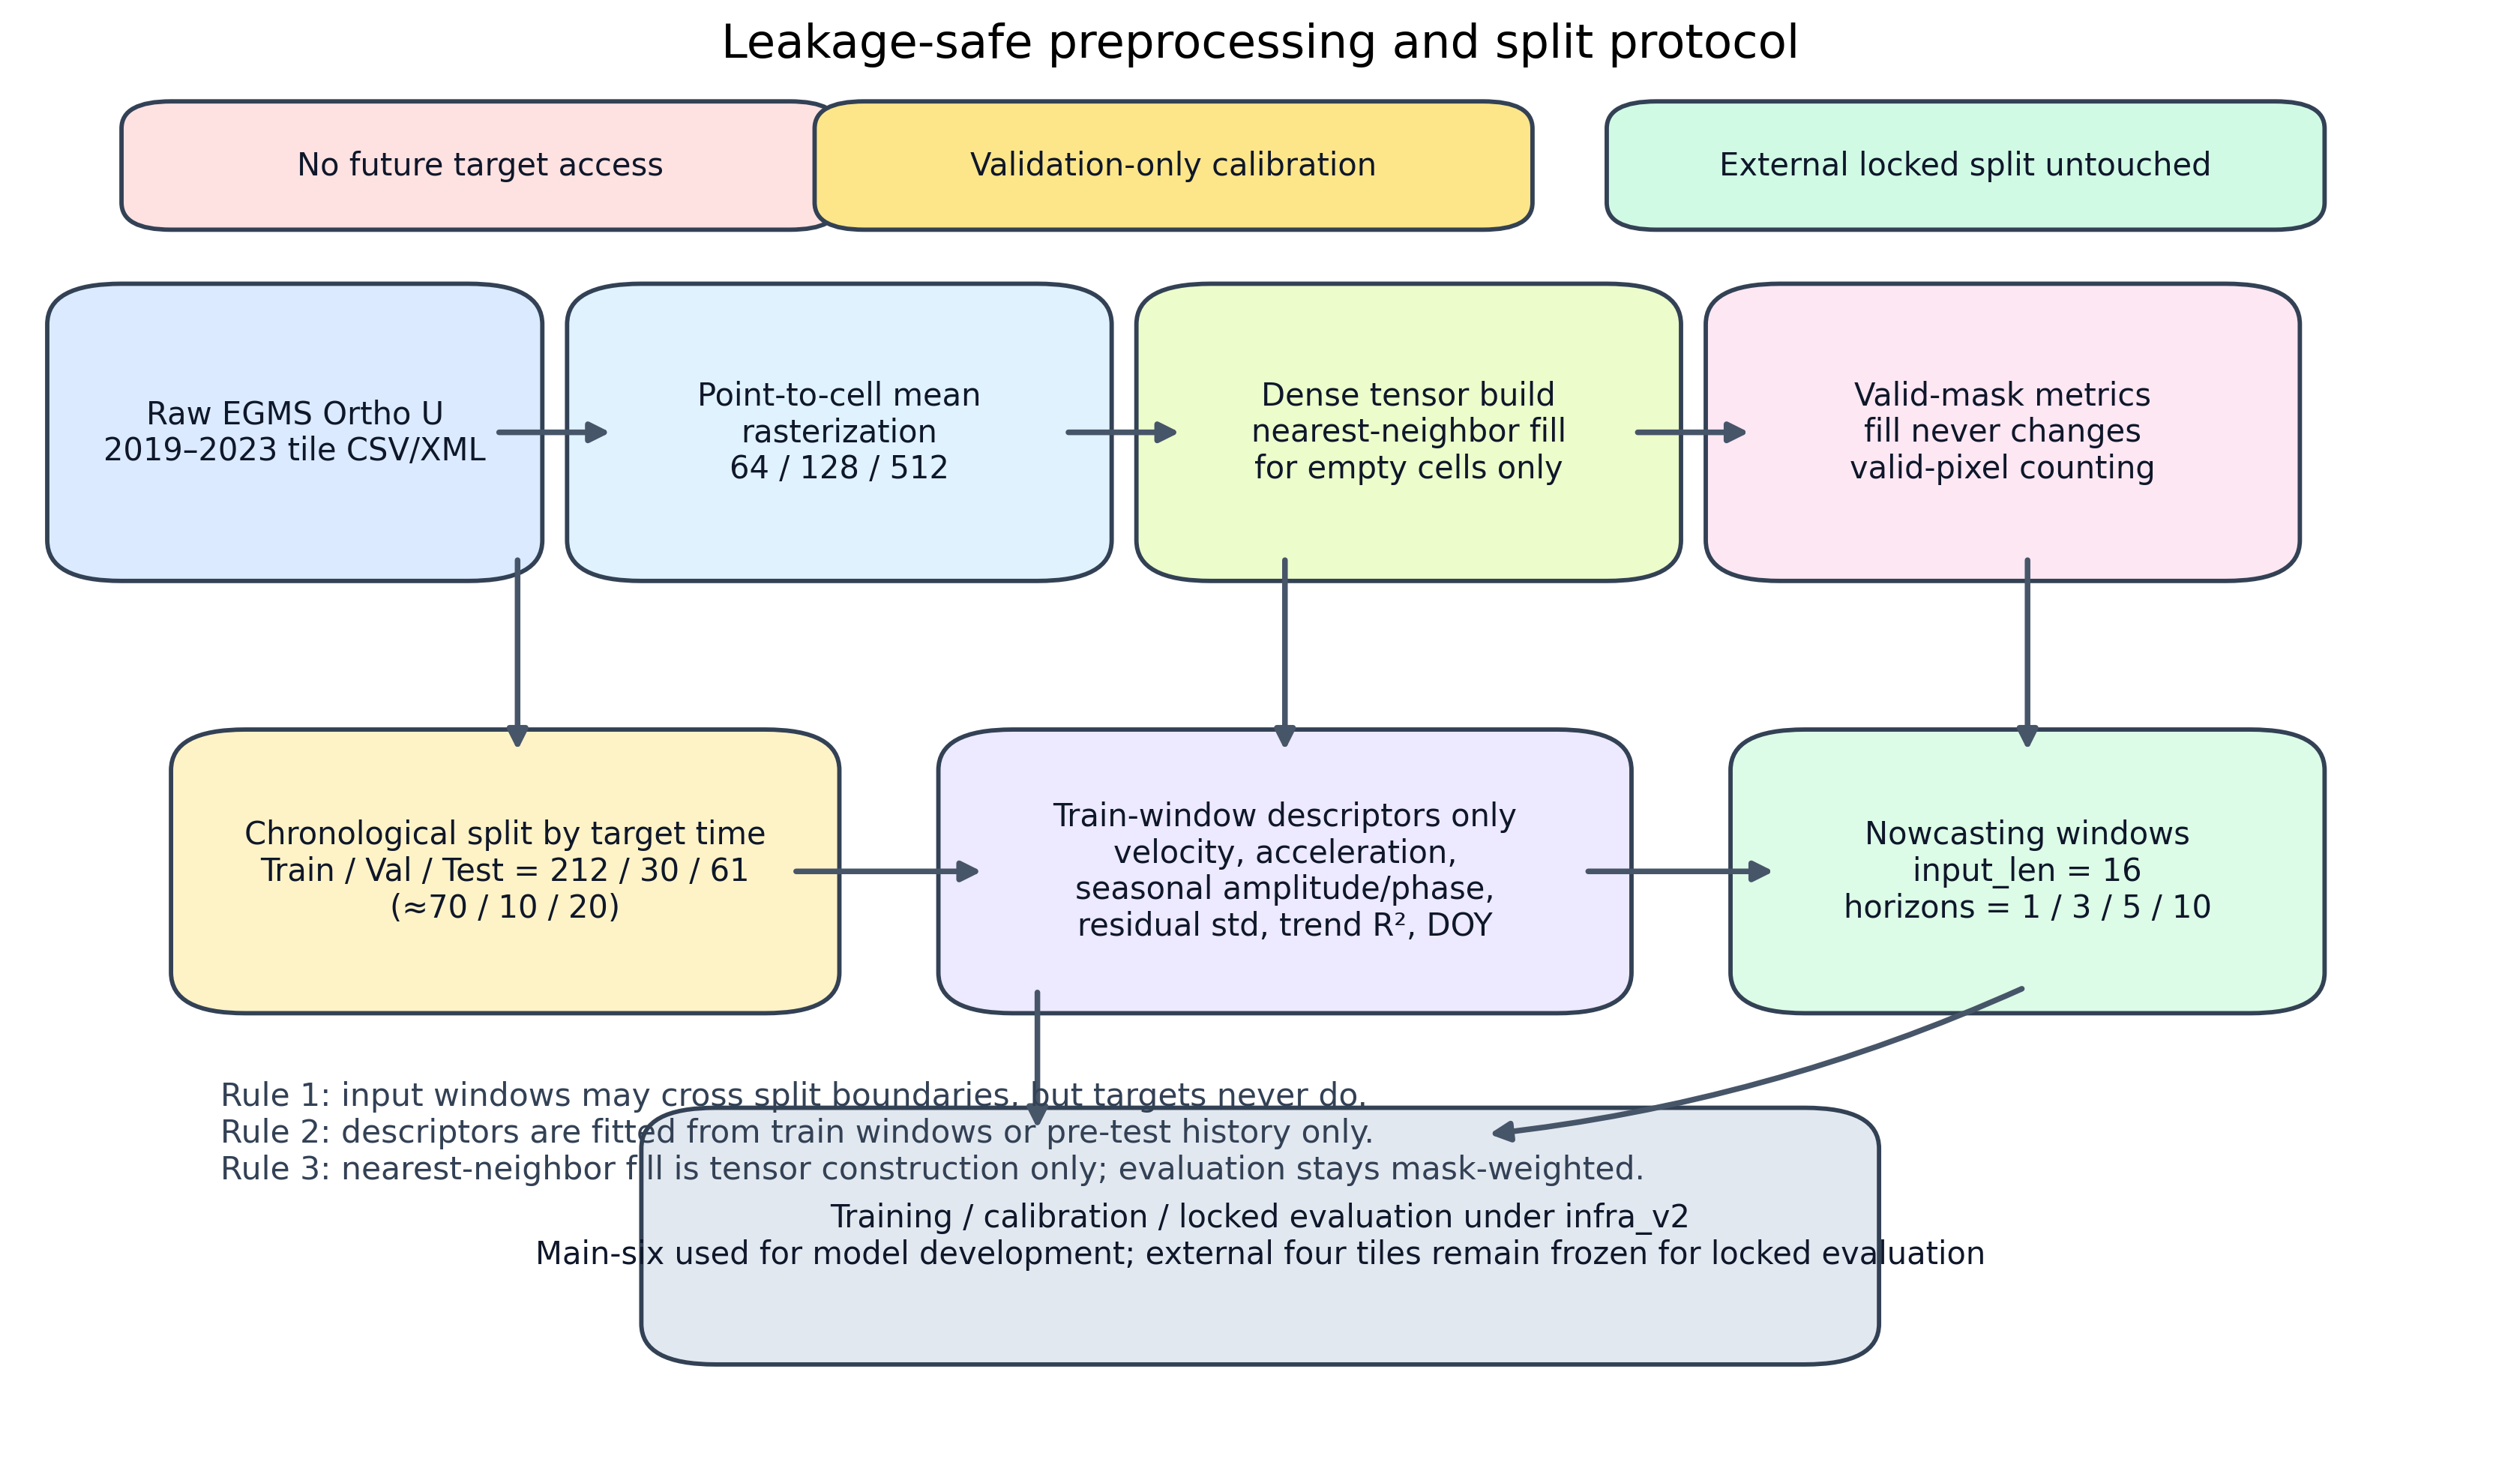
\includegraphics[width=\textwidth,height=0.29\textheight,keepaspectratio]{figures/final/Fig02_leakage_safe_pipeline.png}
  \caption{Leakage-safe preprocessing and split protocol. Raw EGMS point observations were rasterized by point-to-cell mean aggregation, converted into dense tensors with nearest-neighbor fill for empty cells only, and evaluated with valid-mask weighted metrics. Chronological train/validation/test splits were assigned by target time, descriptors were computed from train windows or pre-test history only, and the external locked split remained untouched throughout model search.}
  \label{fig:fig02}
\end{figure*}

\begin{table*}[!t]
  \centering
  \caption{Unified data protocol used throughout the manuscript, including the EGMS product version, split strategy, input length, target horizons, primary and sensitivity resolutions, and descriptor policy.}
  \label{tab:table02}
  \footnotesize
  \begin{adjustbox}{max width=\textwidth}
  \begin{tabular}{p{0.18\textwidth}p{0.18\textwidth}p{0.52\textwidth}}
    \toprule
    \shortstack{Protocol\\item} & Setting & Note \\
    \midrule
    Product & EGMS 2019-2023 Ortho U & All formal results use the unified 2019-2023 Ortho U version. \\
    Main tiles & 6 & E32N34, E32N35, E39N30, E44N23, E48N24, E58N17. \\
    Original external locked tiles & 4 & E37N42, E45N51, E30N35, E42N21. \\
    14-tile frozen audit tiles & 14 & Held-out EGMS 2019--2023 tiles selected by metadata-only stratification after model, calibration, and threshold freeze. \\
    Main split & 70/10/20 chronological & Leakage-safe train/val/test split. \\
    Input length & 16 frames & Unified for the development audit suite and all later mainline experiments. \\
    Horizons & t+1, t+3, t+5, t+10 & Multi-horizon nowcasting. \\
    Main resolution & 64$\times$64 & Primary regional nowcasting setting. \\
    Sensitivity resolutions & 128$\times$128, 512$\times$512 & Sensitivity/robustness only, not the main task. \\
    Descriptors & velocity, acceleration, seasonal amplitude, seasonal phase, residual std, trend R$^2$, DOY sin/cos & Fitted from train-window history or permitted pre-test history only. \\
    Split-protocol controls & target-time, full-window containment, 10-frame gap-buffer & Used to check whether the VCEA advantage is explained by split-boundary leakage. \\
    Masking & valid-mask weighted metrics & Nearest-neighbor fill is for dense tensor construction only. \\
    Cross-site normalization & source-tile stats & Target descriptors still computed from target history. \\
    \bottomrule
  \end{tabular}
  \end{adjustbox}
\end{table*}

\begin{table*}[!t]
  \centering
  \caption{Calibration source by evaluation set. VCEA uses tile-local historical validation calibration followed by frozen future evaluation; future test labels are not used for calibration, expert search, or threshold selection.}
  \label{tab:calibration_source_by_set}
  \scriptsize
  \begin{adjustbox}{max width=\textwidth}
  \begin{tabular}{p{0.18\textwidth}ccp{0.17\textwidth}p{0.18\textwidth}p{0.27\textwidth}}
    \toprule
    Evaluation set & \shortstack{Tile-local\\validation\\weights} & \shortstack{Future\\test\\labels used?} & Expert-search source & SS-VCEA threshold source & Correct interpretation \\
    \midrule
    Main-six development benchmark & Yes & No & development training/validation only & pooled main-six validation risk & historical validation calibration + future test \\
    Original four-tile external audit & Yes & No & fixed before audit & fixed from pooled main-six validation & held-out external future evaluation with tile-local historical calibration \\
    14-tile European frozen audit & Yes & No & fixed before audit & fixed from pooled main-six validation & metadata-stratified held-out European audit with tile-local historical calibration \\
    \bottomrule
  \end{tabular}
  \end{adjustbox}
\end{table*}

\section{Problem Formulation and Metrics}
For tile $s$, target time $t$, and horizon $h\in\{1,3,5,10\}$, the input is a sequence $X_{s,t-L+1:t}$ with $L=16$ frames and associated leakage-safe descriptors. The target is the valid-mask displacement field $Y_{s,t+h}$. Each expert $m\in\mathcal{M}$ outputs $\hat{Y}^{(m)}_{s,t,h}$, and an aggregation method produces $\hat{Y}_{s,t,h}$.

The primary metric is skill over persistence:
\begin{equation}
\mathrm{Skill}_{\mathrm{MSE}} = 1 - \frac{\mathrm{MSE}(\hat{Y},Y)}{\mathrm{MSE}(Y_t,Y)},
\end{equation}
where $Y_t$ is the most recent displacement frame. Positive values indicate improvement over persistence, zero matches persistence, and negative values indicate degradation. We also report RMSE, MAE, thresholded accuracy, SSIM, stress ratio, better-tile counts, and physics-oriented diagnostics. The stress ratio is an operational over-correction and reliability indicator defined relative to the persistence reference. It is not intended to measure geophysical hazard, deformation severity, or engineering risk.

\begin{figure*}[!t]
  \centering
  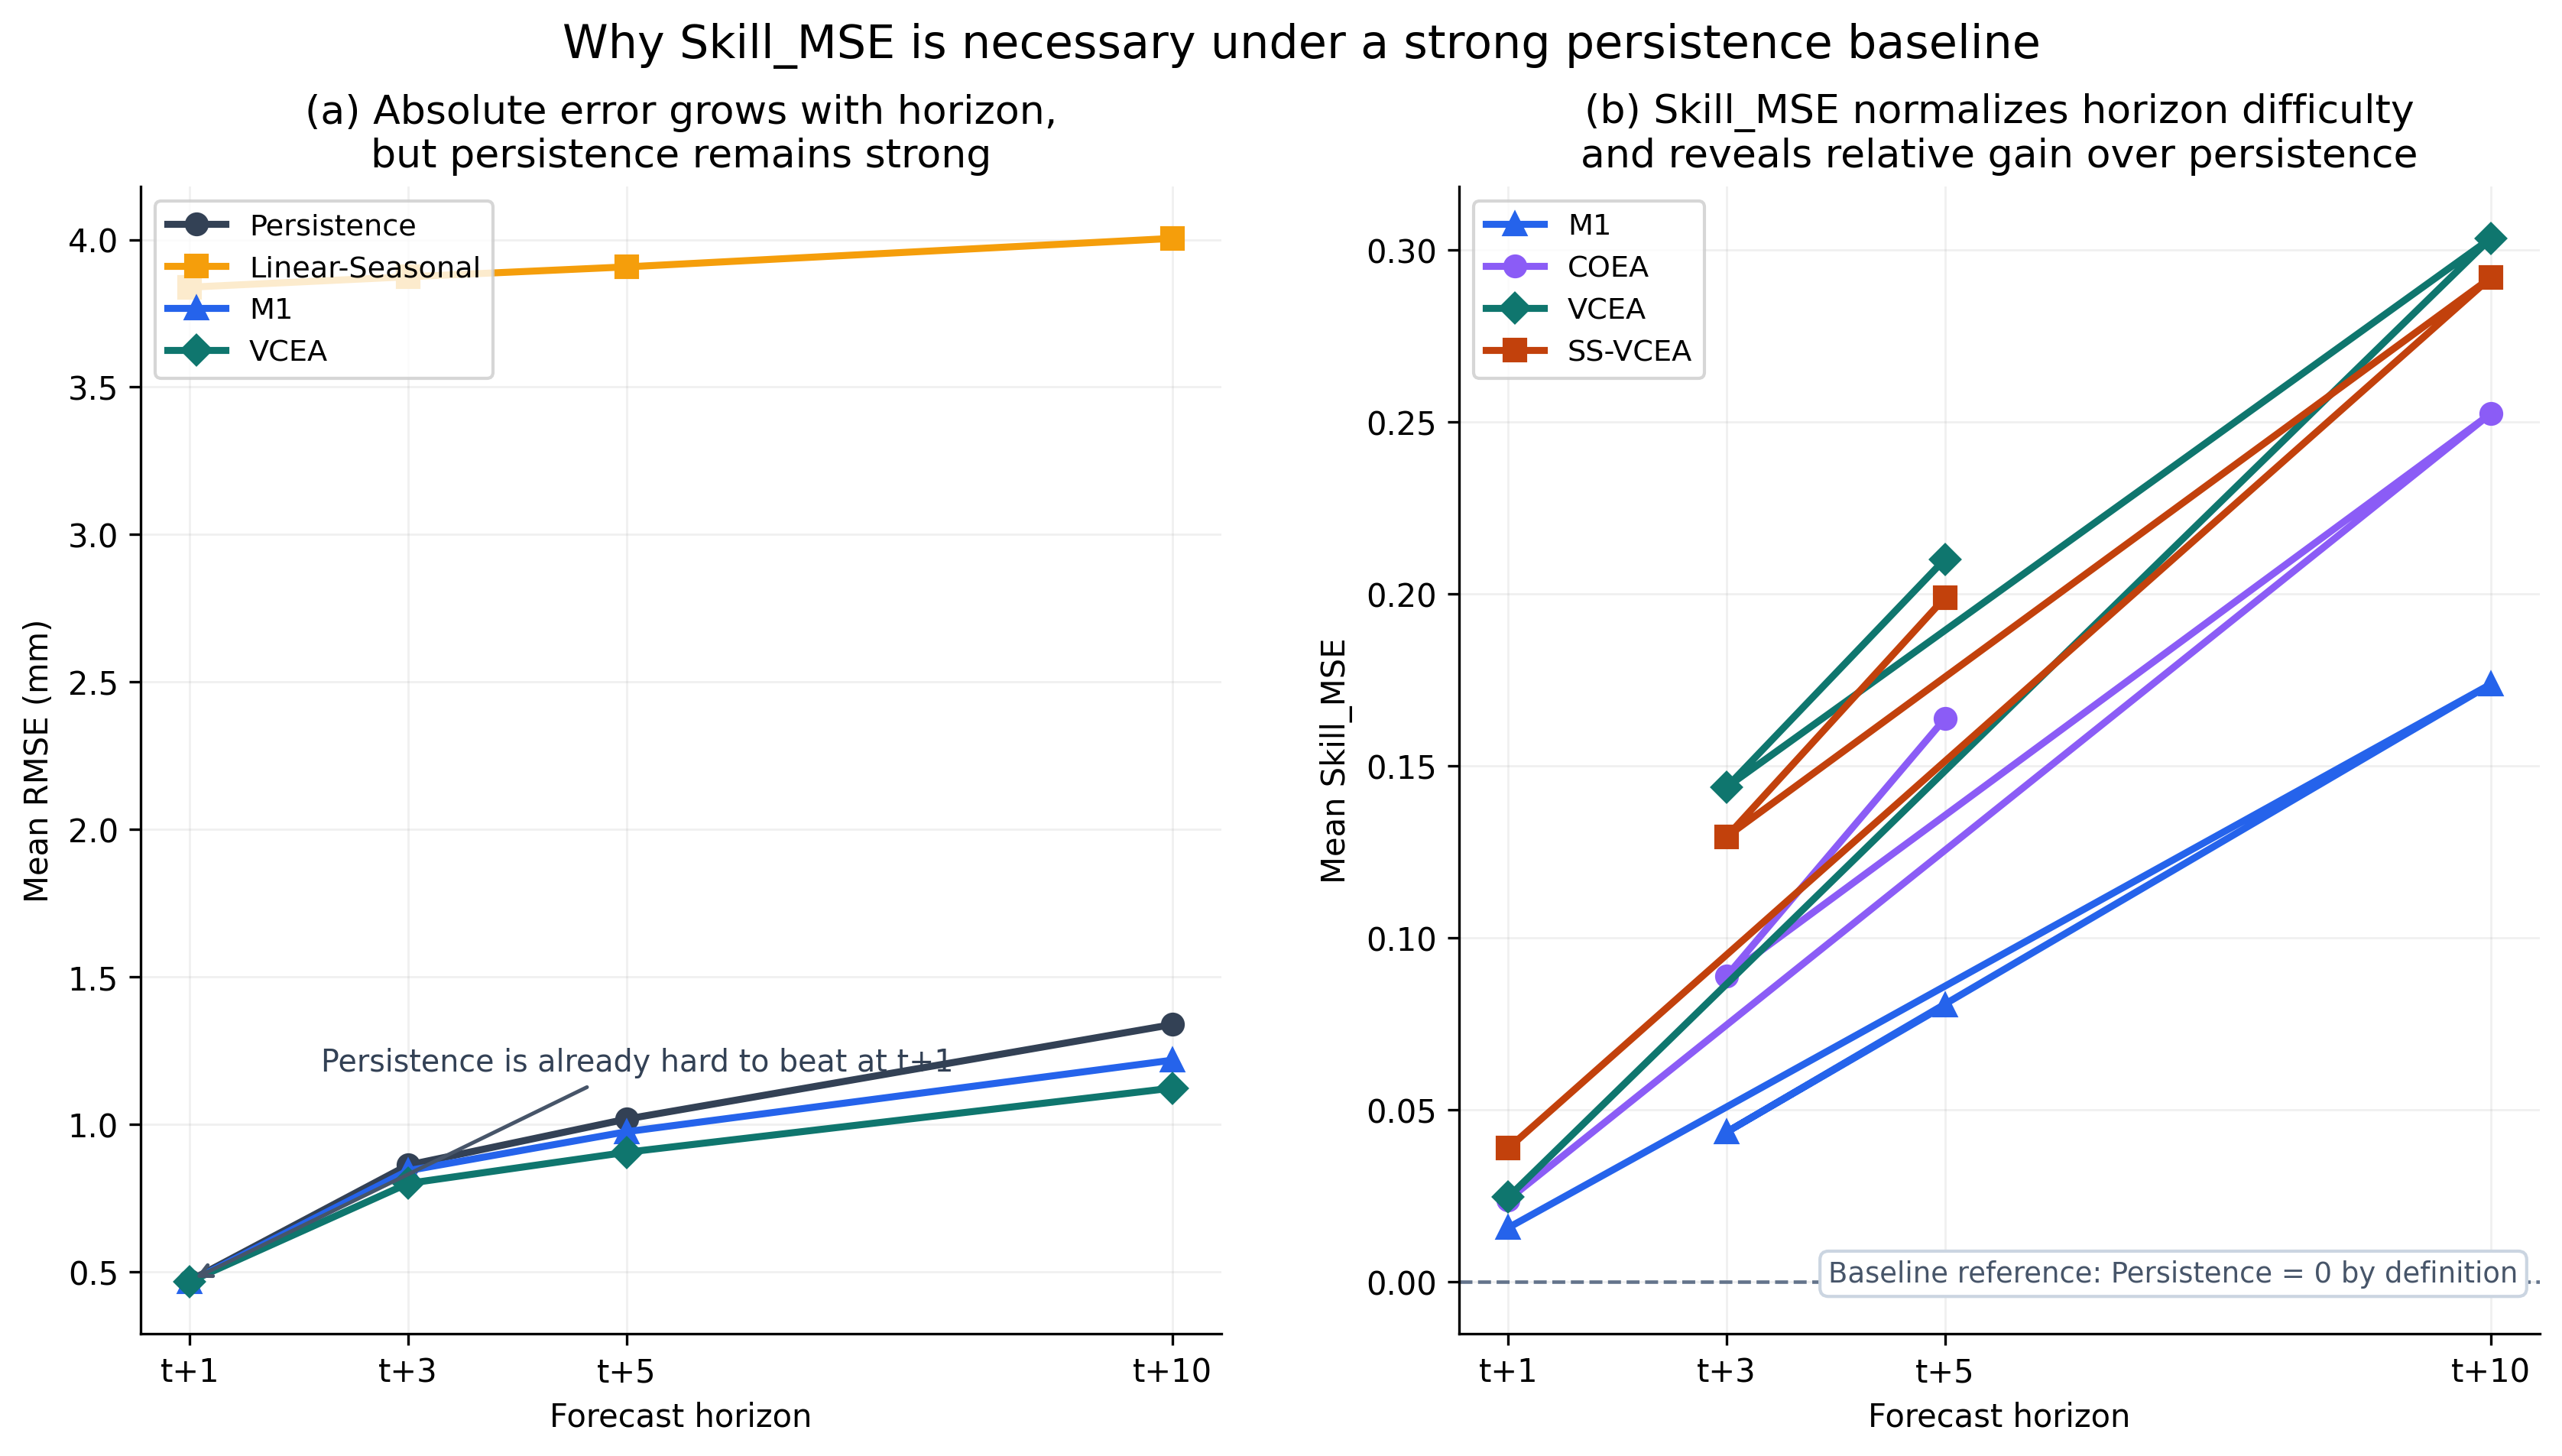
\includegraphics[width=\textwidth,height=0.34\textheight,keepaspectratio]{figures/final/Fig03_persistence_and_horizon_difficulty.png}
  \caption{Why Skill$_{\mathrm{MSE}}$ is required under a strong persistence baseline. (a) Absolute RMSE grows with horizon, but persistence remains highly competitive, especially at $t{+}1$. (b) Skill$_{\mathrm{MSE}}$ normalizes horizon difficulty and makes relative gains over persistence directly comparable across horizons and models.}
  \label{fig:fig03}
\end{figure*}
Additional metric definitions are summarized in Appendix~\ref{app:protocol_metric_details}.

\section{Method}
\subsection{Expert Pool}
The aggregation family operates on a small but deliberately heterogeneous expert pool. Persistence anchors the strong baseline. Linear-seasonal extrapolation provides an explicit kinematic expert. M1/C2 is retained as the best-performing robust neural expert in the evaluated pool after the single-model search. C3\_opt is retained as a complementary higher-capacity expert even though it is not the final standalone model. VCEA and SS-VCEA are not new backbone architectures. They operate above a fixed pool of persistence, kinematic, online, and neural experts and study whether validation-calibrated aggregation can improve EGMS displacement-map nowcasting under a strong persistence baseline. A compact summary of the evaluated experts and baselines is provided in Appendix~\ref{app:protocol_metric_details}.

\subsection{Validation-Calibrated Expert Aggregation}
VCEA calibrates one static expert mixture for each tile and horizon using validation losses only. Let $L^{\mathrm{val}}_{s,h,m}$ denote the validation MSE of expert $m$ on tile $s$ and horizon $h$, and let expert $m=0$ denote persistence. The implementation first normalizes each expert loss by the persistence loss,
\begin{equation}
\tilde{L}_{s,h,m}=\frac{L^{\mathrm{val}}_{s,h,m}}{\max(L^{\mathrm{val}}_{s,h,0},\varepsilon)},
\end{equation}
then applies inverse-loss weighting
\begin{equation}
u_{s,h,m}=\left(\max(\tilde{L}_{s,h,m},\varepsilon)\right)^{-\tau},
\end{equation}
followed by normalization and shrinkage toward the uniform prior:
\begin{equation}
\bar{w}_{s,h,m}=(1-\rho)\frac{u_{s,h,m}}{\sum_{j\in\mathcal{M}}u_{s,h,j}}+\rho\frac{1}{|\mathcal{M}|}.
\end{equation}
An optional floor can reserve a minimum mass for the M1 expert. Let $w_{s,h,m}$ denote the post-floor weights. In the selected mainline configuration, \texttt{floor0p0} disables this constraint, so $w_{s,h,m}=\bar{w}_{s,h,m}$. The final prediction is
\begin{equation}
\hat{Y}^{\mathrm{VCEA}}_{s,t,h}=\sum_{m\in\mathcal{M}} w_{s,h,m}\hat{Y}^{(m)}_{s,t,h}.
\end{equation}
The implementation identifier of the selected configuration is \texttt{StaticVal\_inverse\_temp4p0\_sh0p1\_floor0p0}, corresponding to inverse weighting with $\tau=4.0$, shrinkage $\rho=0.1$, and zero minimum M1 floor. This identifier is retained only as a reproducibility tag. Because these weights are estimated from validation losses only and then frozen, VCEA avoids both oracle selection and test-time retuning.
For the main-six benchmark, the original external audit, and the 14-tile audit, these weights are always estimated from historical validation windows on the corresponding tile and then frozen for future evaluation. Held-out tiles are therefore excluded from expert search, threshold selection, future-test tuning, and final configuration choice, but not from tile-local historical validation calibration.

\subsection{COEA and SS-VCEA}
COEA is a causal online aggregation baseline initialized from validation information and updated under delayed feedback. It is useful as a comparison because it tests whether online adaptation is necessary. During evaluation, COEA updates are allowed only after the corresponding target frame becomes observable under the simulated release schedule; no target label is used to update weights before producing the forecast for that target. In this benchmark, COEA improves over M1 but remains weaker than VCEA, which motivates the validation-transfer stability analysis in Section~VI.

SS-VCEA keeps the VCEA prediction as the accuracy anchor and applies a validation-calibrated hard fallback when a normalized risk score is high. The fallback branch used throughout the manuscript is COEA. For each pixel and horizon, three normalized quantities are evaluated:
\begin{align}
d_{s,t,h} &= \frac{|\hat{Y}^{\mathrm{VCEA}}_{s,t,h}-\hat{Y}^{\mathrm{COEA}}_{s,t,h}|}{\max(\sigma^{\mathrm{res}}_{s},0.1)},\\
c_{s,t,h} &= \frac{|\hat{Y}^{\mathrm{VCEA}}_{s,t,h}-\hat{Y}^{\mathrm{pers}}_{s,t,h}|}{\max(\sigma^{\mathrm{res}}_{s},0.1)},\\
v_{s,t,h} &= \frac{\sigma^{\mathrm{res}}_{s}}{\max(\mathrm{median}(\sigma^{\mathrm{res}}_{s'}),0.1)},
\end{align}
where $\sigma^{\mathrm{res}}_{s}$ is the residual-standard-deviation descriptor estimated from the available training history. The equal-normalized risk score is then
\begin{equation}
r_{s,t,h}=\frac{d_{s,t,h}+c_{s,t,h}+v_{s,t,h}}{3}.
\end{equation}
For each horizon $h$, a threshold $\tau_h$ is calibrated as the 97.5th percentile of the corresponding validation-risk distribution from the main-six tiles. The selected operating point is therefore denoted SS-VCEA q97.5, and the final prediction is a hard switch:
\begin{equation}
\hat{Y}^{\mathrm{SS}}_{s,t,h}=
\begin{cases}
\hat{Y}^{\mathrm{COEA}}_{s,t,h}, & r_{s,t,h}>\tau_h,\\
\hat{Y}^{\mathrm{VCEA}}_{s,t,h}, & \text{otherwise}.
\end{cases}
\end{equation}
SS-VCEA q97.5 therefore uses per-horizon thresholds derived from the pooled main-six validation risk distribution, and these thresholds are held fixed for the main test, the original external audit, and the 14-tile audit. The q97.5 variant is selected as a conservative operating point from the validation-only threshold sweep, not as the highest-skill threshold. SS-VCEA is thus reported as a conservative operating variant, not as a default replacement for VCEA. Stress reduction in this setting should be interpreted as lower forecasting over-correction pressure rather than as lower physical deformation risk.

\begin{figure*}[!t]
  \centering
  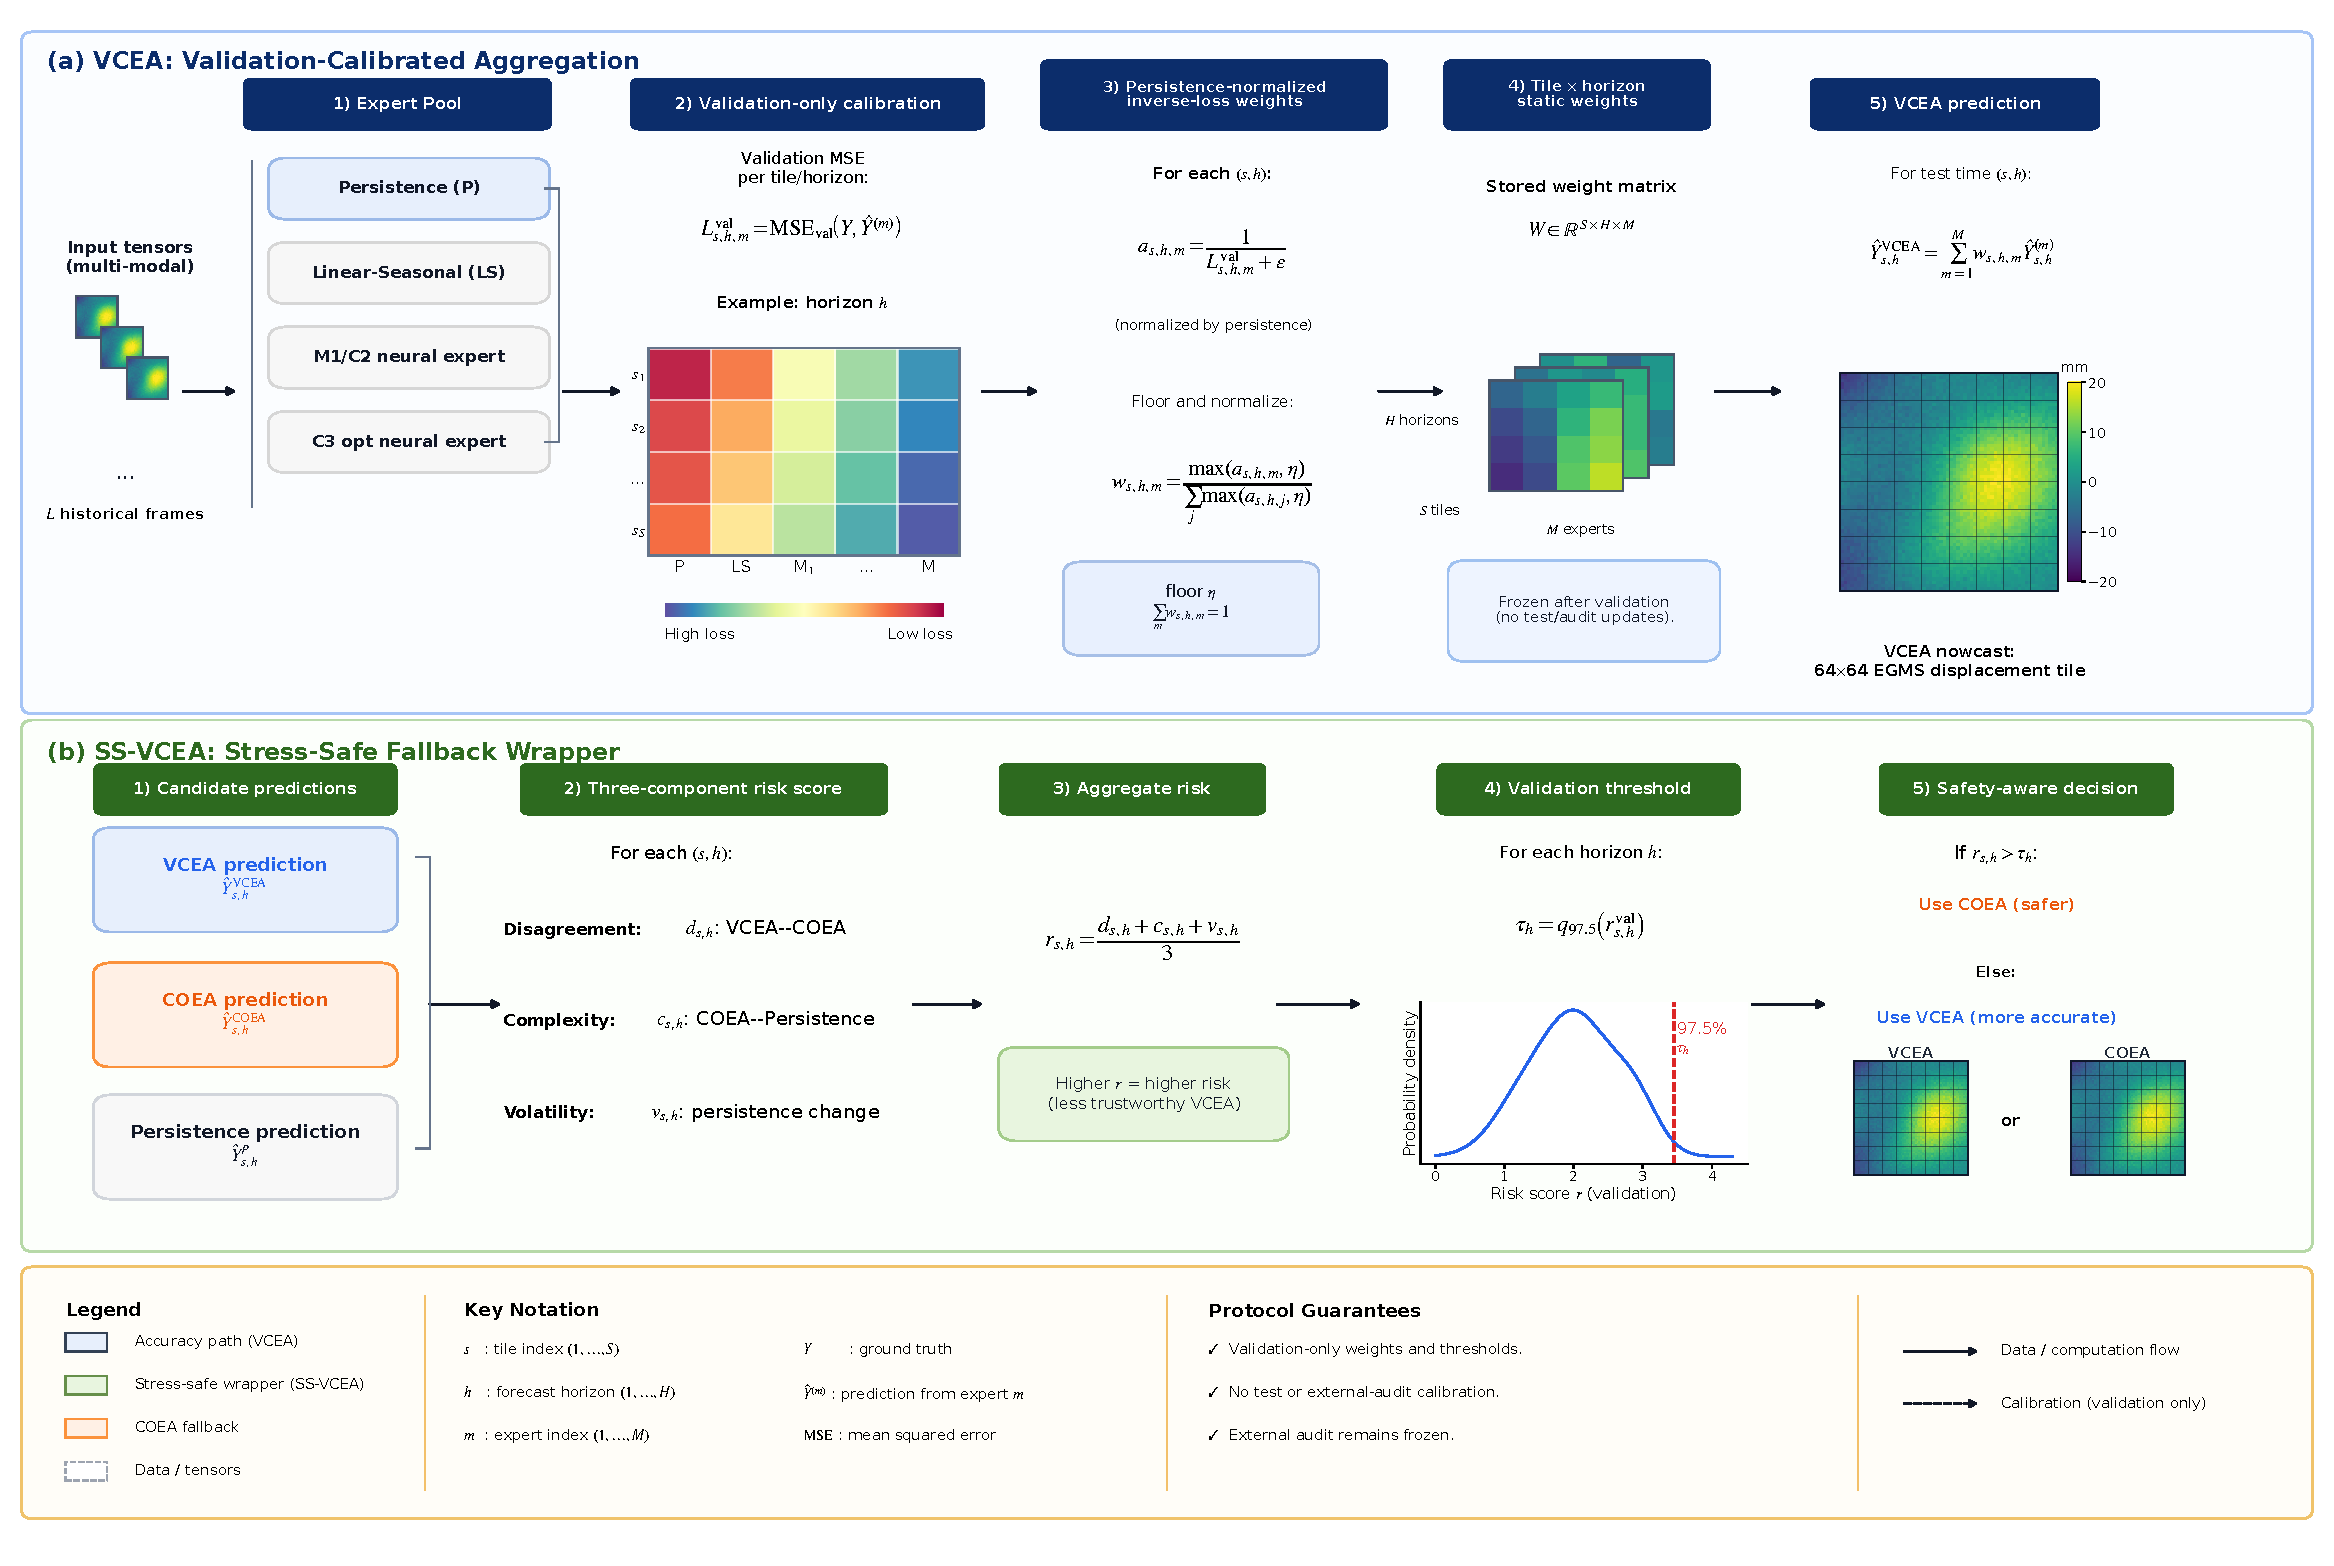
\includegraphics[width=\textwidth,height=0.36\textheight,keepaspectratio]{figures/final/Fig04_vcea_ssvcea_method.pdf}
  \caption{Method overview of VCEA and SS-VCEA. VCEA performs validation-only static expert calibration over the expert pool $\{\text{Persistence},\text{Linear-Seasonal},\text{M1/C2},\text{C3 opt}\}$ and produces a tile$\times$horizon-specific weighted prediction. SS-VCEA reuses the same expert pool and applies a validation-calibrated hard fallback when the equal-normalized risk score $r=(d+c+v)/3$ exceeds a horizon-specific threshold.}
  \label{fig:fig04}
\end{figure*}
An explicit protocol-comparison table is provided in Appendix~\ref{app:protocol_metric_details}.

\section{Experiments and Results}
\subsection{Main Development Benchmark}
The main-six comparison shows that aggregation, rather than any single expert, is the most effective strategy in this benchmark. VCEA reaches mean \skillmse{} 0.178 and improves over M1 by 0.099. COEA also improves over M1, reaching 0.132, but the static validation-calibrated VCEA mixture remains stronger. SS-VCEA q97.5 reaches 0.165 and outperforms M1 on all six main tiles while reducing stress relative to VCEA. A tile-horizon heatmap for the four primary comparison models is provided in Appendix~\ref{app:protocol_metric_details}.

\begin{table*}[!t]
  \centering
  \caption{Main-six comparison of the primary baselines, neural experts, and aggregation methods under the exact $64\times64$ setting.}
  \label{tab:table06}
  \scriptsize
  \begin{adjustbox}{max width=\textwidth}
  \begin{tabular}{llrrrrrp{0.22\textwidth}}
    \toprule
    Model & Category & \shortstack{Mean\\Skill$_{\mathrm{MSE}}$} & \shortstack{Gain\\vs M1} & \shortstack{Better tiles\\vs M1} & \shortstack{Stress\\ratio} & \shortstack{Seed\\std} & Note \\
    \midrule
    VCEA & aggregation & 0.178 & 0.099 & 6 & 1.046 & 0.010 & main-six exact comparison \\
    SS-VCEA q97.5 & fallback-controlled aggregation & 0.165 & 0.086 & 6 & 0.992 & 0.020 & selected conservative operating variant \\
    COEA & aggregation & 0.132 & 0.054 & 6 & 0.996 & 0.021 & main-six exact comparison \\
    CRCF-COEA & aggregation & 0.127 & 0.049 & 6 & 1.002 & 0.022 & main-six exact comparison \\
    C3\_opt & neural expert & 0.080 & 0.001 & 2 & 0.992 & 0.020 & full-six near-pass expert \\
    M1 & baseline & 0.078 & -0.000 & 4 & 1.002 & 0.021 & main-six exact comparison \\
    Persistence & baseline & 0.000 & -0.078 & 0 & 1.000 & 0.000 & main-six exact comparison \\
    Linear-Seasonal & kinematic baseline & -36.149 & -36.228 & 0 & 16.845 & 0.000 & strong explicit kinematic baseline \\
    \bottomrule
  \end{tabular}
  \end{adjustbox}
\end{table*}

The large negative value of the standalone linear-seasonal baseline reflects unbounded extrapolation under some tile-horizon conditions. It is therefore diagnostic as a single expert, while VCEA controls its contribution through validation-calibrated weights.

\subsection{Split-Protocol and Leakage Audit}
Table~\ref{tab:e1_leakage_audit} and Fig.~\ref{fig:e1_skill_delta_by_tile} summarize the split-protocol audit. Under the main target-time assignment, VCEA improves over M1 by 0.099 in mean \skillmse{}. The gain remains positive under full-window containment (0.079) and the 10-frame gap-buffer protocol (0.085), even though these stricter protocols reduce the number of admissible validation and test windows. This supports the interpretation that the primary aggregation benefit is not explained by split-boundary leakage. The stress ratio changes under stricter protocols, so the skill advantage is robust but the SS-VCEA threshold should be recalibrated if the operational split protocol changes.

\begin{table*}[!t]
\centering
\scriptsize
\begin{adjustbox}{max width=\textwidth}
\begin{tabular}{lp{0.13\textwidth}rrrrp{0.21\textwidth}}
\toprule
Protocol & Val/Test windows & VCEA Skill$_{\mathrm{MSE}}$ & M1 Skill$_{\mathrm{MSE}}$ & VCEA gain & SS-VCEA stress ratio & Interpretation \\
\midrule
Target-time assignment & 120 / 306 & 0.178 & 0.078 & 0.099 & 0.992 & main online protocol; positive gain retained \\
Full-window containment & 30 / 216 & 0.159 & 0.080 & 0.079 & 1.152 & stricter containment; positive gain retained \\
Gap-buffer (10 frames) & 60 / 246 & 0.170 & 0.085 & 0.085 & 1.133 & stricter buffer; positive gain retained \\
\bottomrule
\end{tabular}
\end{adjustbox}
\caption{Leakage-audit comparison across the main target-time assignment and two stricter split protocols. VCEA retains positive gain over M1 under full-window containment and a ten-frame gap buffer, supporting the interpretation that the aggregation advantage is not an artifact of target-time assignment. The full audit table and detailed window-rule definitions are reproduced in Appendix~\ref{app:e1_e3_full_tables}.}
\label{tab:e1_leakage_audit}
\end{table*}

\begin{figure*}[!t]
\centering
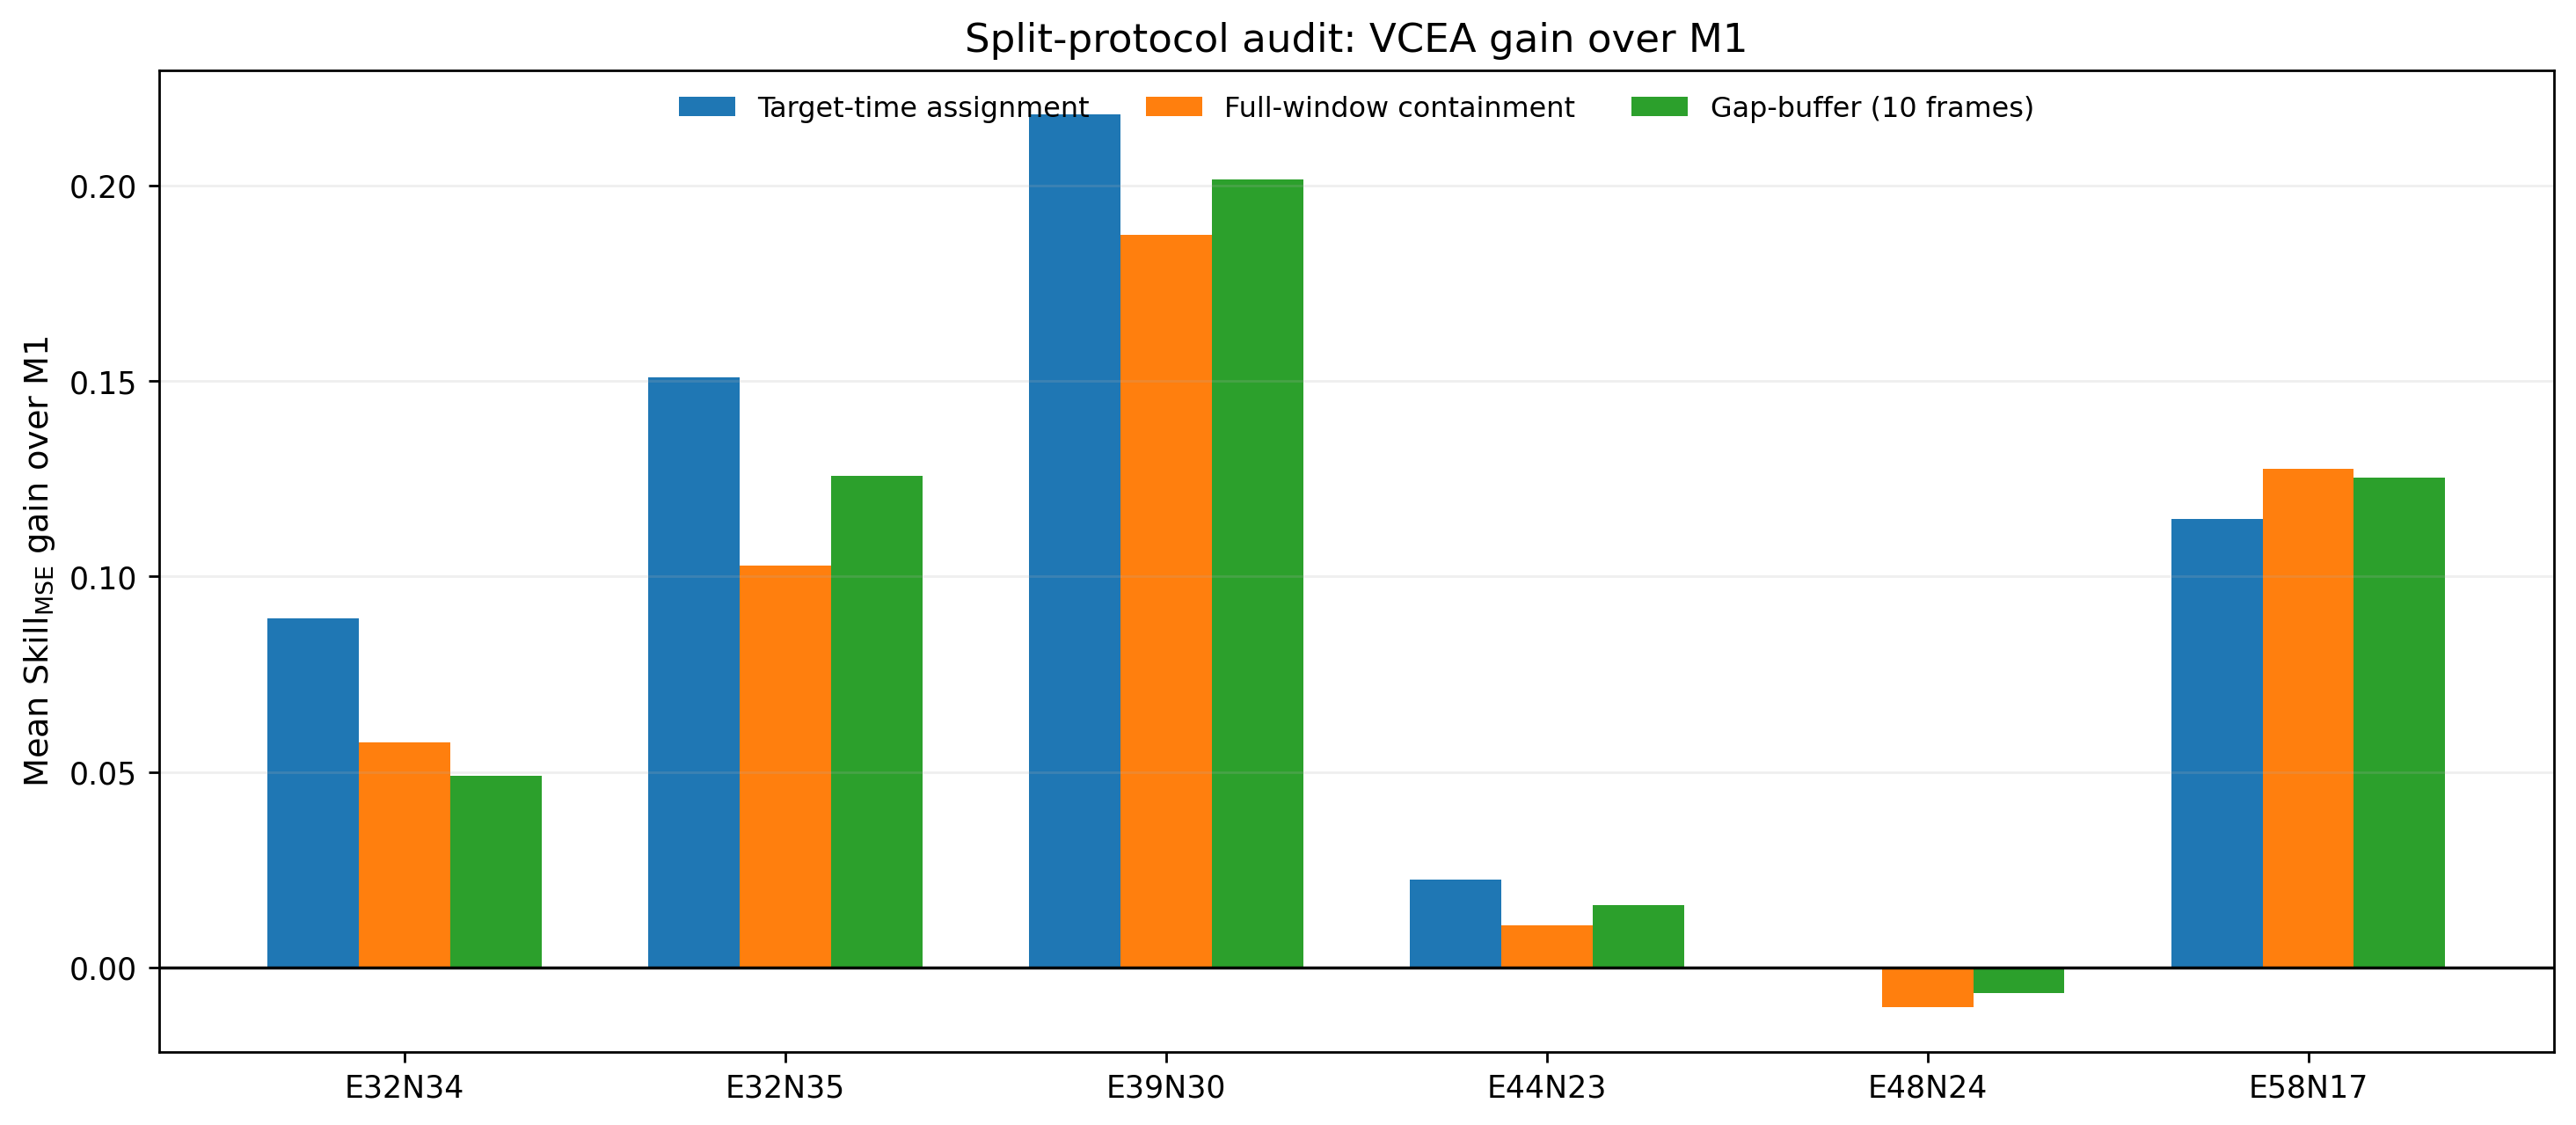
\includegraphics[width=0.95\textwidth]{paper_assets_vcea_extras/figures/E1/fig_E1_skill_delta_by_tile.png}
\caption{Tile-wise VCEA gain over M1 under the split-protocol audit. Gains remain positive under stricter protocols, supporting the interpretation that VCEA does not rely on target-time assignment artifacts.}
\label{fig:e1_skill_delta_by_tile}
\end{figure*}

\subsection{Contribution of Heterogeneous Experts}
Table~\ref{tab:e2_expert_ablation_main6} and Fig.~\ref{fig:e2_expert_weights} show that the full heterogeneous pool is important. Full VCEA outperforms the removal variants on the main-six setting, while uniform expert averaging becomes strongly negative in main-six \skillmse{} and exhibits high stress. Removing the linear-seasonal expert degrades skill substantially, indicating that explicit kinematic structure is useful even though the standalone linear-seasonal baseline is weak. Removing M1 or C3\_opt also degrades performance, showing that neural experts provide complementary value when used as candidate experts rather than as the sole contribution.

\begin{table*}[!t]
\centering
\footnotesize
\begin{adjustbox}{max width=\textwidth}
\begin{tabular}{lp{0.22\textwidth}rrrrp{0.18\textwidth}}
\toprule
Variant & Removed or changed component & Main-six Skill$_{\mathrm{MSE}}$ & External Skill$_{\mathrm{MSE}}$ & Stress ratio & Better tiles & Interpretation \\
\midrule
VCEA\_full & none & 0.178 & 0.317 & 1.046 & 6 & full pool reference \\
without\_C3\_opt & remove complementary higher-capacity neural expert & 0.158 & 0.323 & 1.093 & 5 & skill decreases even with M1 retained \\
without\_M1 & remove robust neural expert & 0.155 & 0.307 & 1.082 & 4 & skill decreases when the main neural expert is removed \\
without\_linear\_seasonal & remove explicit kinematic expert & 0.112 & 0.174 & 0.996 & 5 & kinematic structure contributes to the mixture \\
uniform\_expert\_average & same expert pool, no learned calibration & -1.805 & 0.267 & 4.112 & 3 & uniform averaging performs poorly \\
\bottomrule
\end{tabular}
\end{adjustbox}
\caption{Compact expert-pool ablation on the main-six setting. The full VCEA pool outperforms the key removal variants, while uniform averaging is not a reliable substitute. The complete ablation table, including the persistence-removal and single-family diagnostic variants, is reproduced in Appendix~\ref{app:e1_e3_full_tables}.}
\label{tab:e2_expert_ablation_main6}
\end{table*}

\begin{figure*}[!t]
\centering
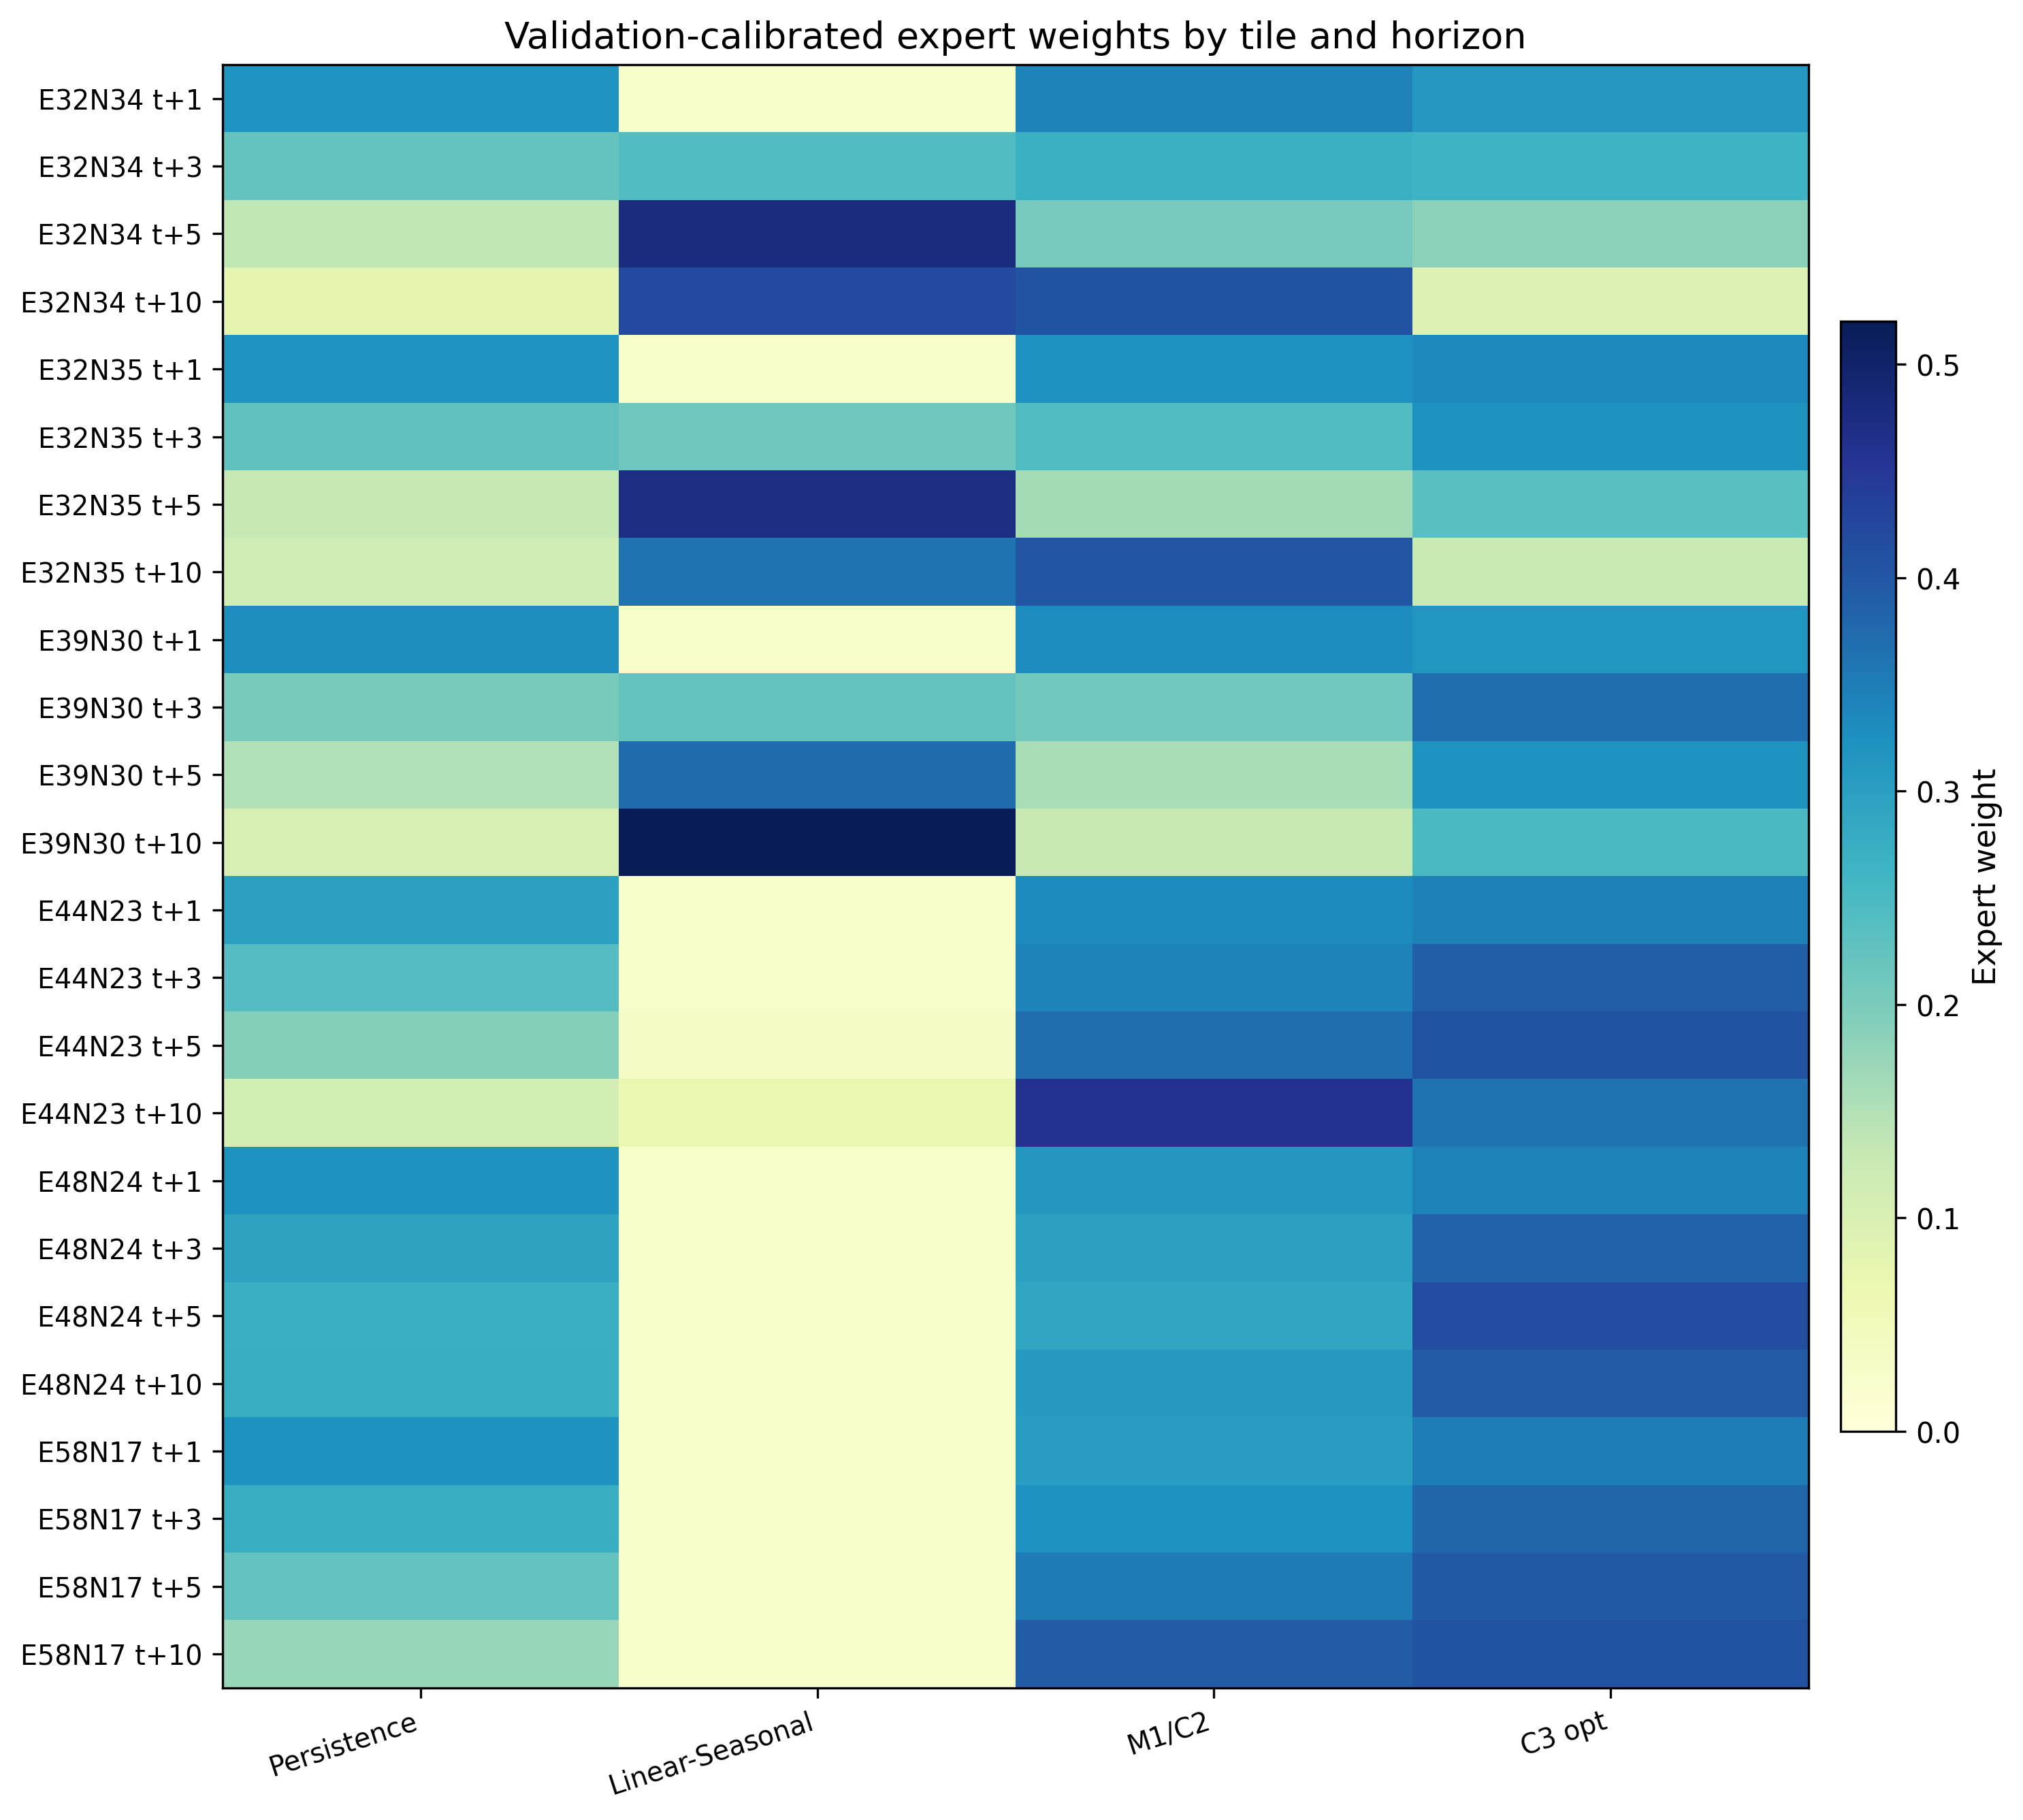
\includegraphics[width=0.95\textwidth]{paper_assets_vcea_extras/figures/E2/fig_E2_expert_weights_heatmap.png}
\caption{Validation-calibrated expert weights by tile and horizon. VCEA does not reduce to a uniform average and instead shifts trust across persistence, linear-seasonal, and neural experts according to tile-horizon conditions.}
\label{fig:e2_expert_weights}
\end{figure*}

\subsection{Role of Tile- and Horizon-Aware Calibration}
The calibration ablation in Table~\ref{tab:e3_calibration_ablation} and Fig.~\ref{fig:e3_calibration_barplot} separates the role of validation weighting from the expert pool itself. Global validation weights improve over uniform averaging, but the full tile- and horizon-aware calibration gives the best main-six result in this benchmark and the smallest oracle gap. Tile-only and horizon-only calibration both contribute, and horizon-only calibration is slightly higher on the original external set; therefore, the full VCEA configuration is best interpreted as the best overall trade-off in this benchmark rather than as the best value for every single submetric.

\begin{table*}[!t]
\centering
\footnotesize
\begin{adjustbox}{max width=\textwidth}
\begin{tabular}{lcccrrrr}
\toprule
Aggregation & Calibration source & Tile-aware & Horizon-aware & Main-six Skill$_{\mathrm{MSE}}$ & External Skill$_{\mathrm{MSE}}$ & Stress ratio & Oracle gap \\
\midrule
Uniform average & uniform & -- & -- & -1.805 & 0.267 & 4.112 & 2.002 \\
Global validation weights & validation & -- & -- & 0.129 & 0.281 & 1.051 & 0.067 \\
Tile-only VCEA & validation & \checkmark & -- & 0.154 & 0.255 & 1.046 & 0.042 \\
Horizon-only VCEA & validation & -- & \checkmark & 0.133 & 0.320 & 1.047 & 0.063 \\
Full tile+horizon VCEA & validation & \checkmark & \checkmark & 0.178 & 0.317 & 1.046 & 0.019 \\
Oracle test weights & test-oracle & \checkmark & \checkmark & 0.196 & 0.356 & 0.996 & 0.000 \\
\bottomrule
\end{tabular}
\end{adjustbox}
\caption{Calibration ablation for validation-based expert aggregation. Checkmarks indicate whether calibration varies by tile or horizon. Full tile+horizon validation calibration yields the best main-six result in this benchmark and the smallest oracle gap, whereas uniform averaging is insufficient under the strong persistence baseline. The full calibration table is reproduced in Appendix~\ref{app:e1_e3_full_tables}.}
\label{tab:e3_calibration_ablation}
\end{table*}

\begin{figure*}[!t]
\centering
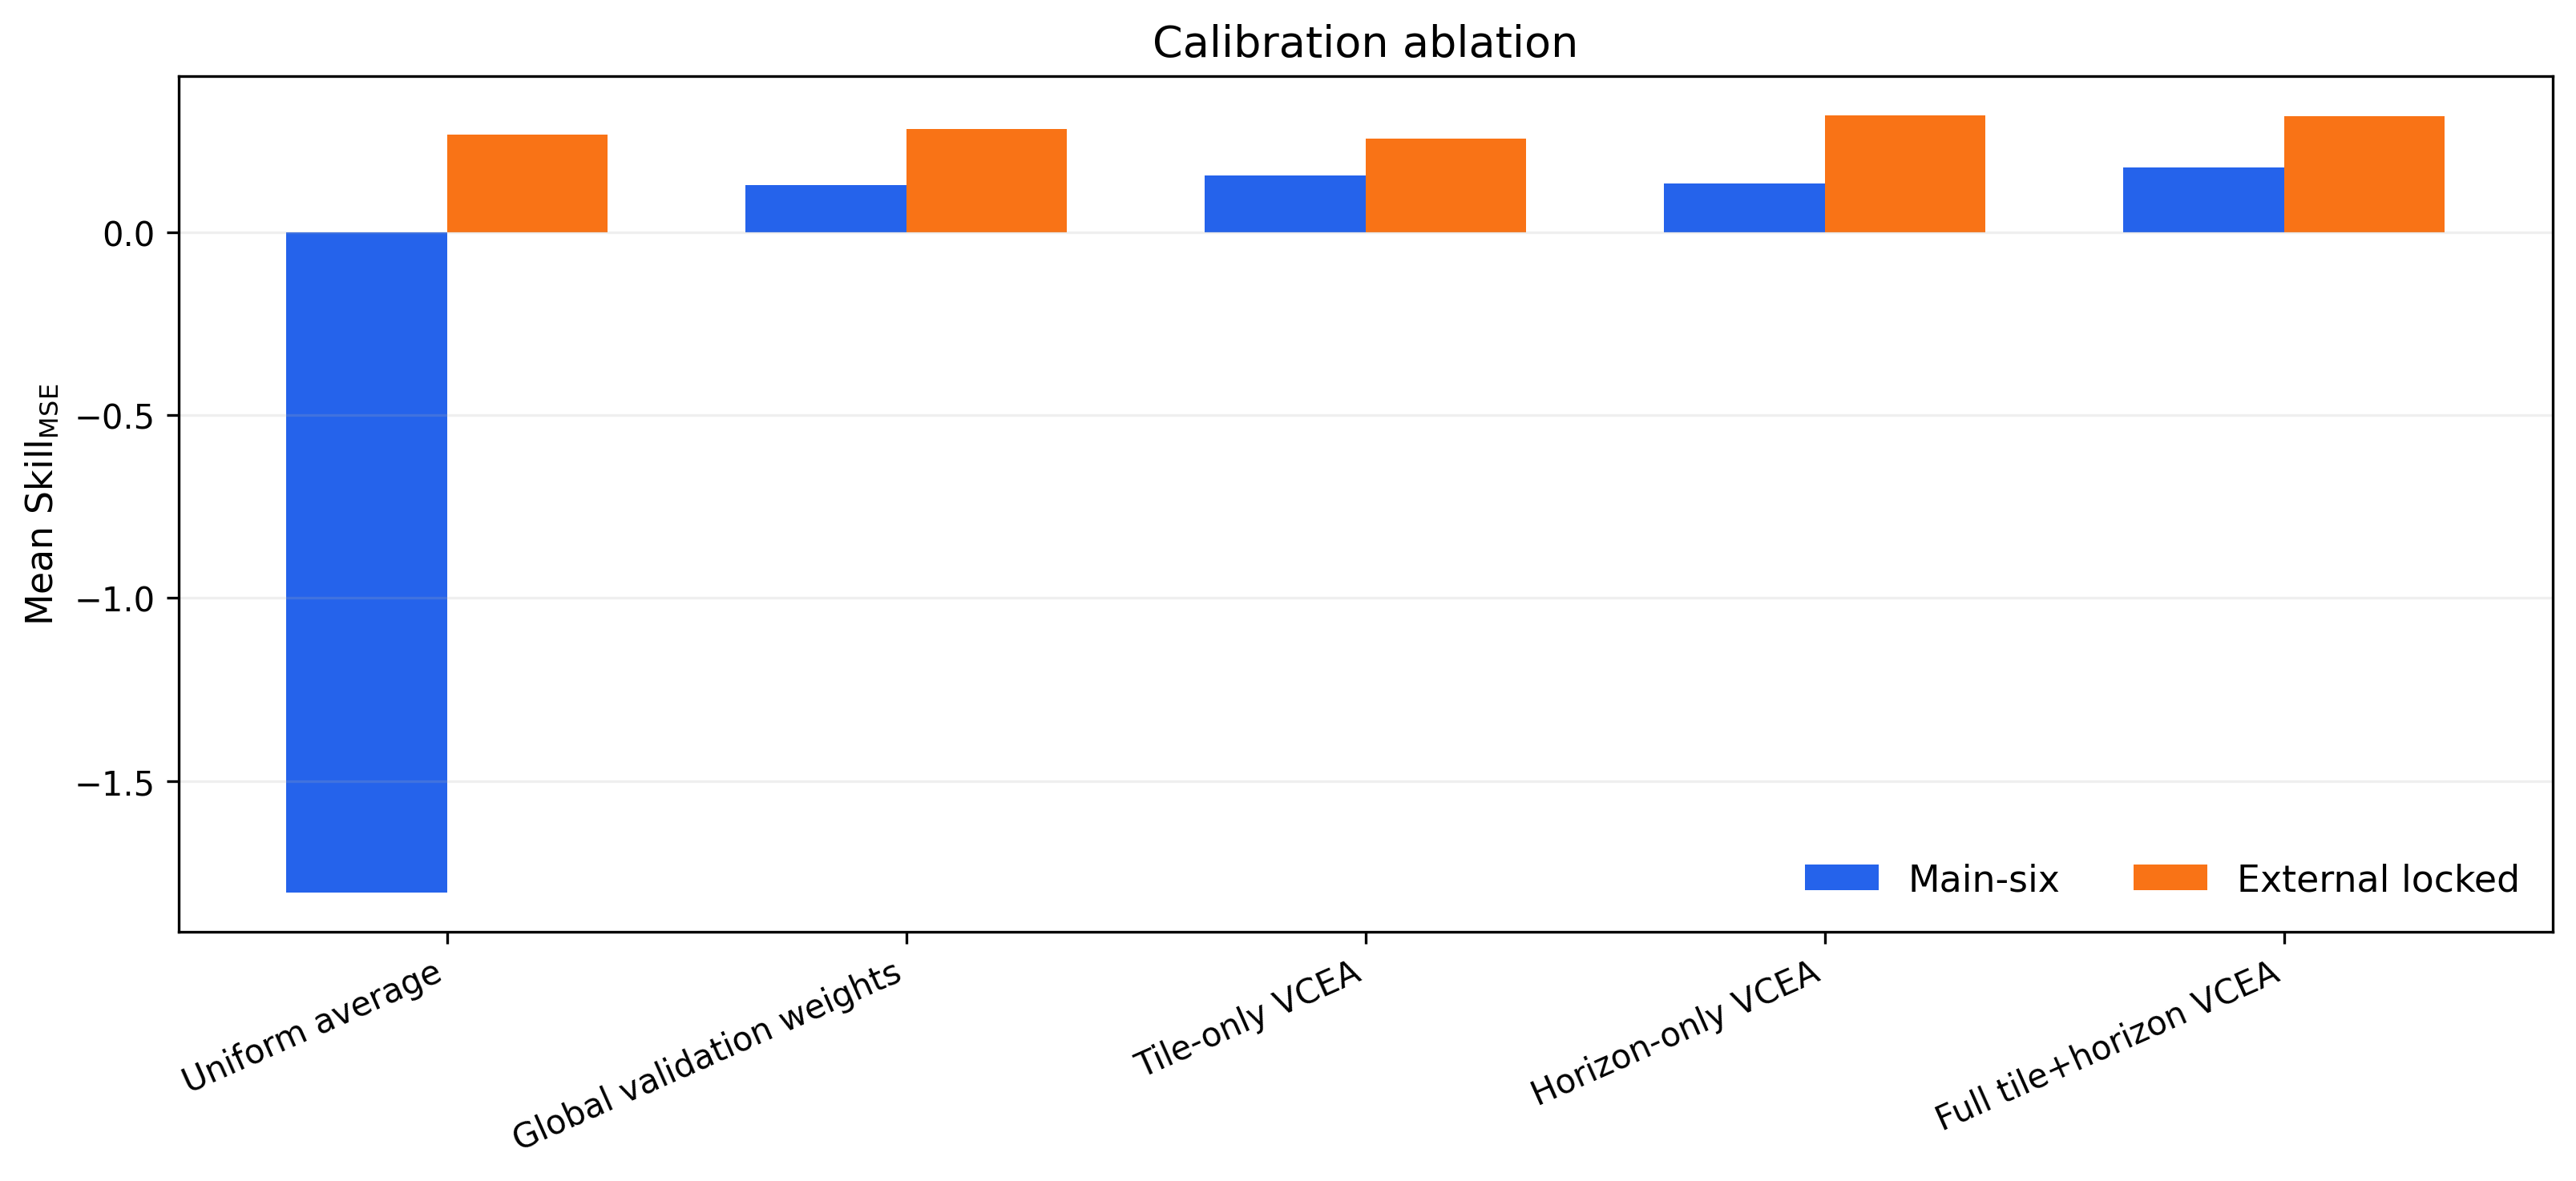
\includegraphics[width=0.95\textwidth]{paper_assets_vcea_extras/figures/E3/fig_E3_calibration_barplot.png}
\caption{Calibration-ablation summary across aggregation strategies. Full tile+horizon validation calibration achieves the best main-six skill in this benchmark and the smallest oracle gap, whereas uniform averaging is insufficient under the strong persistence baseline.}
\label{fig:e3_calibration_barplot}
\end{figure*}

\subsection{Validation-Transfer and Blocked-Validation Robustness}
Blocked-validation robustness tests whether VCEA is merely adapted to one validation interval. Short validation blocks still produce positive test-period performance, although the middle block is weaker and blocked weights are less stable than full-validation weights. VTSA provides the mechanism-level explanation: expert rankings on validation are strongly aligned with expert rankings on test, with mean Spearman correlation 0.778, mean Kendall correlation 0.731, and top-2 retention 0.917. In contrast, the online COEA weights show substantial L1 drift relative to the static validation mixture, consistent with performance loss under delayed feedback. Together, these results support using the full validation period for the frozen calibration and indicate that VCEA is not solely an accidental fit to a single validation split. The compact blocked-validation table, VTSA summary, and supporting weight-stability figures are placed in Appendix~\ref{app:blocked_validation_vtsa}.

\subsection{Skill--Stress Operating Point}
Table~\ref{tab:e6_threshold_sweep} and Fig.~\ref{fig:e6_skill_stress_frontier} report the SS-VCEA threshold sweep. The selected q97.5 operating point preserves skill close to VCEA while reducing the main-six stress ratio below one with a modest fallback rate. The q99 setting gives slightly higher mean skill but a smaller operating margin, whereas q90 and q95 are more conservative but lose more skill. SS-VCEA is therefore a conservative fallback layer, not a new model optimized only for highest average accuracy.

\begin{table*}[!t]
\centering
\footnotesize
\begin{adjustbox}{max width=\textwidth}
\begin{tabular}{lrrrrrl}
\toprule
Threshold & Skill$_{\mathrm{MSE}}$ & Stress ratio & Fallback rate & Correction magnitude & Worse tiles & Selected? \\
\midrule
no\_fallback & 0.178 & 1.046 & 0.000 & 0.000 & 0 & no \\
q90 & 0.161 & 0.992 & 0.157 & 0.056 & 5 & no \\
q95 & 0.171 & 0.991 & 0.102 & 0.043 & 3 & no \\
q97.5 & 0.178 & 0.992 & 0.070 & 0.033 & 3 & yes \\
q99 & 0.179 & 0.997 & 0.040 & 0.021 & 3 & no \\
\bottomrule
\end{tabular}
\end{adjustbox}
\caption{Threshold sweep for SS-VCEA. The selected q97.5 operating point preserves skill close to VCEA while reducing stress below one with a modest fallback rate, making it the preferred conservative operating point. Although q99 gives slightly higher mean skill, q97.5 is used as the selected conservative operating point because it keeps the stress ratio below one with minimal skill loss.}
\label{tab:e6_threshold_sweep}
\end{table*}

\begin{figure*}[!t]
\centering
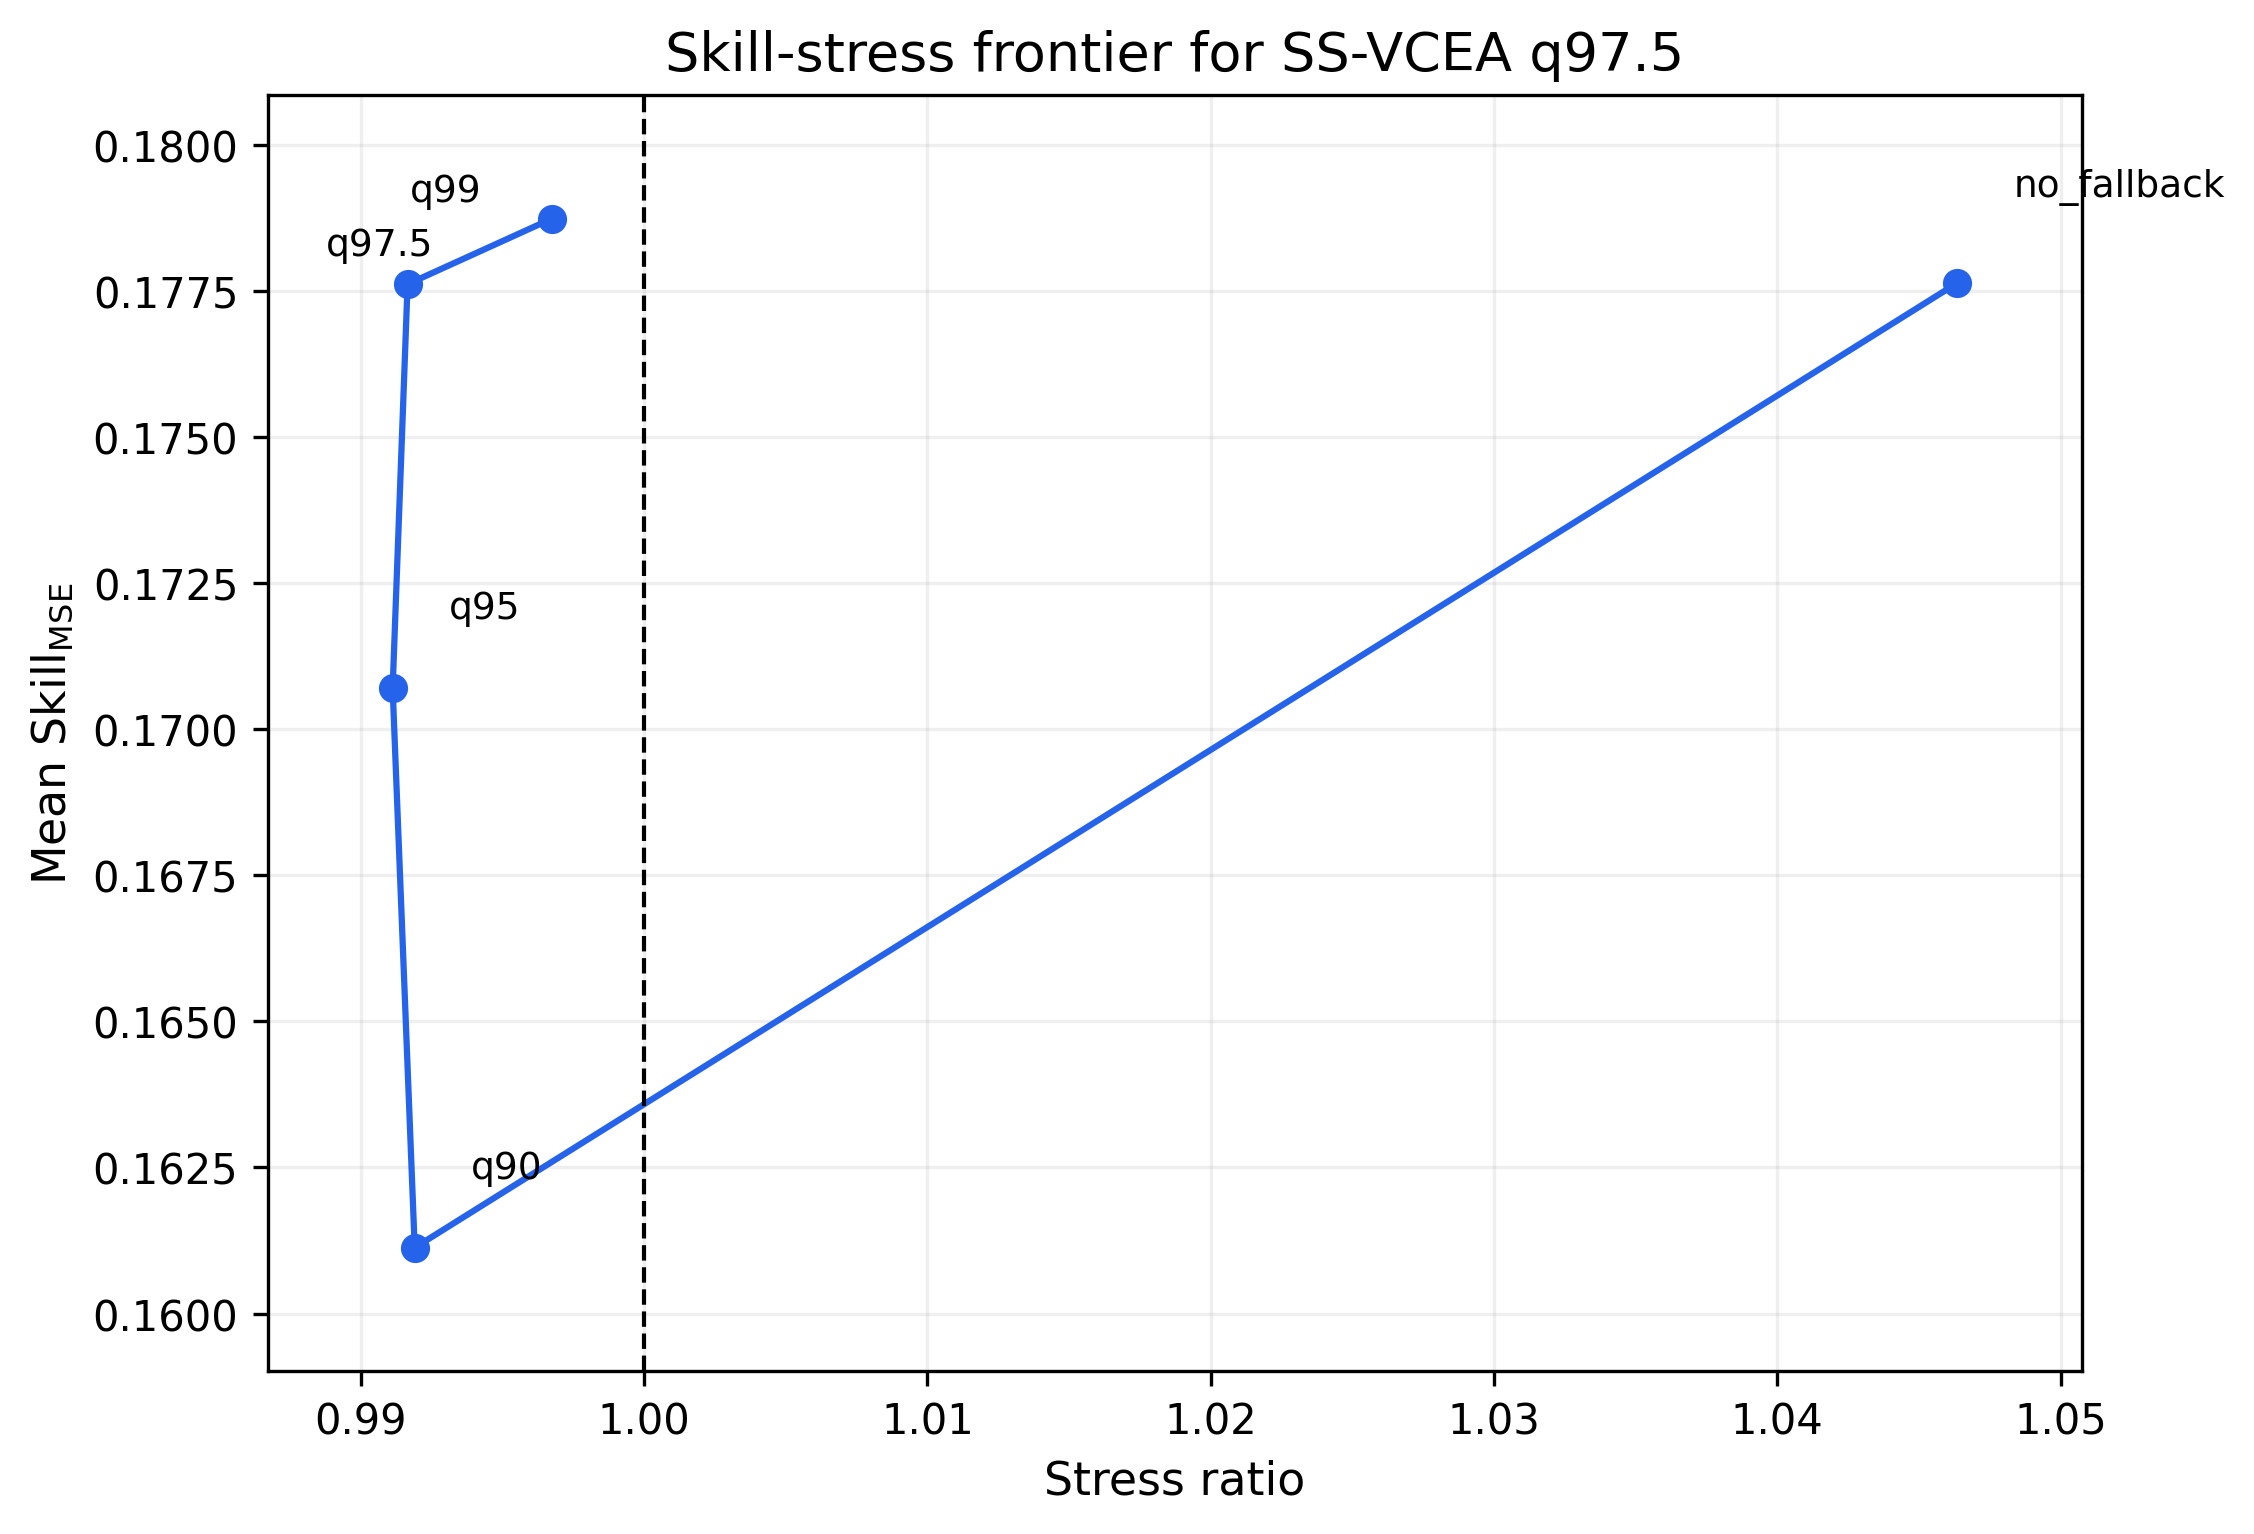
\includegraphics[width=0.95\textwidth]{paper_assets_vcea_extras/figures/E6/fig_E6_skill_stress_frontier.png}
\caption{Skill--stress frontier for the SS-VCEA threshold sweep. The selected q97.5 operating point keeps skill close to VCEA while reducing stress below one, supporting its use as the main conservative operating setting.}
\label{fig:e6_skill_stress_frontier}
\end{figure*}

\subsection{Matched Conservative Operating-Point Reference}
VCEA is the best-performing configuration in the evaluated main-six setting, but its main-six stress ratio is higher than that of the selected conservative fallback variant. A matched operating-point reference recomputation is therefore used only to compare VCEA and SS-VCEA under the same reference package, so the VCEA main-six value in that package is 0.171 rather than the primary 0.178 reported in Table~\ref{tab:table06}. Within this matched reference, SS-VCEA q97.5 reduces the main-six stress ratio to 0.992 with a modest mean \skillmse{} loss of 0.006. The corresponding matched-reference table is provided in Appendix~\ref{app:safety_resolution}; it is not the primary main-six claim.

\subsection{Original Four-Tile Frozen External Audit}
The four original external tiles remain held out for expert search, threshold selection, and final configuration choice. Under the frozen expert pool, frozen threshold logic, and tile-local historical validation calibration, each external tile uses only its own historical validation windows to estimate aggregation weights before future test evaluation. Under this held-out external future-evaluation protocol, VCEA reaches external mean \skillmse{} of 0.317, compared with 0.160 for M1 and 0.083 for C3\_opt. This result supports positive held-out future-evaluation performance of the aggregation family, but it should not be interpreted as a broad continental claim because the external set is finite and dominated by mixed-regime tiles. The full original four-tile summary and the matched operating-point reference recomputation are provided in Appendix~\ref{app:safety_resolution}.

\subsection{Geographically Stratified 14-Tile European Frozen Audit}
To evaluate external future performance beyond the development benchmark and the original four-tile external check, we use a geographically stratified 14-tile European audit. The audit contains 14 held-out EGMS 2019--2023 tiles and 56 tile-horizon evaluations selected using metadata-only criteria across six broad-region strata, four audit-regime groups, and three coverage groups. Expert definitions, preprocessing, evaluation metrics, VCEA calibration rules, and SS-VCEA q97.5 thresholds are fixed before this audit. Each audit tile uses only its tile-local historical validation windows to estimate aggregation weights, followed by frozen future evaluation. This protocol therefore evaluates held-out European tiles under historical validation calibration, and it should not be interpreted as exhaustive validation over all European deformation conditions.

Table~\ref{tab:e7_strong_group_summary} reports the compact group summary. Overall, VCEA improves mean \skillmse{} from 0.113 for M1 to 0.260 and reduces mean RMSE from 1.067 mm to 0.866 mm. VCEA improves over M1 on all 14 held-out tiles. SS-VCEA q97.5 preserves most of this gain with mean \skillmse{} 0.229 and a stress ratio of 0.997, while VCEA has stress ratio 0.998. A descriptive statistical audit from the existing by-tile table is provided in Appendix~\ref{app:e7_statistical_audit}: the tile-level sign test yields 14/14 positive gains with two-sided $p=1.22\times10^{-4}$, and the paired tile-level bootstrap gives a mean gain of 0.147 with a 95\% confidence interval of [0.089, 0.217]. These diagnostics are intended as a robustness audit over held-out tiles rather than as a population-level inference over all European deformation conditions. The group rows show positive mean future-evaluation gain within each tested broad-region stratum, audit-regime group, and coverage group. Figs.~\ref{fig:e7_pan_europe_tile_map}, \ref{fig:e7_skill_by_region}, and \ref{fig:e7_skill_vs_coverage} summarize the audit geography, broad-region skill, and coverage dependence.

\begin{table*}[!t]
\centering
\scriptsize
\begin{adjustbox}{max width=\textwidth}
\begin{tabular}{llrrrrrrrr}
\toprule
Type & Group & Tiles & M1 Skill & VCEA Skill & Gain & SS Skill & VCEA SR & SS SR \\
\midrule
overall & all & 14 & 0.113 & 0.260 & 0.147 & 0.229 & 0.998 & 0.997 \\
broad\_region & Alpine/Mountain & 2 & 0.109 & 0.177 & 0.068 & 0.178 & 0.985 & 0.985 \\
broad\_region & Central/Continental & 3 & 0.036 & 0.244 & 0.208 & 0.233 & 0.980 & 0.982 \\
broad\_region & Mediterranean/Southern & 2 & 0.232 & 0.256 & 0.025 & 0.281 & 0.986 & 0.986 \\
broad\_region & Mediterranean/Tectonic & 3 & 0.082 & 0.134 & 0.052 & 0.135 & 0.998 & 0.997 \\
broad\_region & Northern/Nordic & 2 & 0.209 & 0.579 & 0.370 & 0.374 & 0.945 & 0.948 \\
broad\_region & Northwest/Atlantic & 2 & 0.061 & 0.241 & 0.179 & 0.222 & 0.981 & 0.982 \\
audit\_regime\_group & mixed-general & 6 & 0.133 & 0.349 & 0.216 & 0.276 & 0.981 & 0.982 \\
audit\_regime\_group & seasonal-mixed & 5 & 0.123 & 0.242 & 0.119 & 0.245 & 0.986 & 0.986 \\
audit\_regime\_group & sparse-support & 2 & 0.057 & 0.110 & 0.054 & 0.108 & 0.998 & 0.997 \\
audit\_regime\_group & subsidence-mixed & 1 & 0.051 & 0.114 & 0.064 & 0.109 & 0.985 & 0.985 \\
coverage\_group & higher-coverage & 5 & 0.135 & 0.372 & 0.237 & 0.287 & 0.980 & 0.982 \\
coverage\_group & lower-coverage & 5 & 0.078 & 0.161 & 0.083 & 0.156 & 0.998 & 0.997 \\
coverage\_group & middle-coverage & 4 & 0.129 & 0.245 & 0.116 & 0.249 & 0.985 & 0.985 \\
\bottomrule
\end{tabular}
\end{adjustbox}
\caption{Compact summary of the geographically stratified 14-tile European frozen audit on 14 held-out EGMS 2019--2023 tiles, corresponding to 56 tile-horizon evaluations. Skill columns report Skill$_{\mathrm{MSE}}$ and SR denotes stress ratio. RMSE and better-tile counts are discussed in the main text and retained in the appendix-level audit package.}
\label{tab:e7_strong_group_summary}
\end{table*}

\begin{figure*}[!t]
\centering
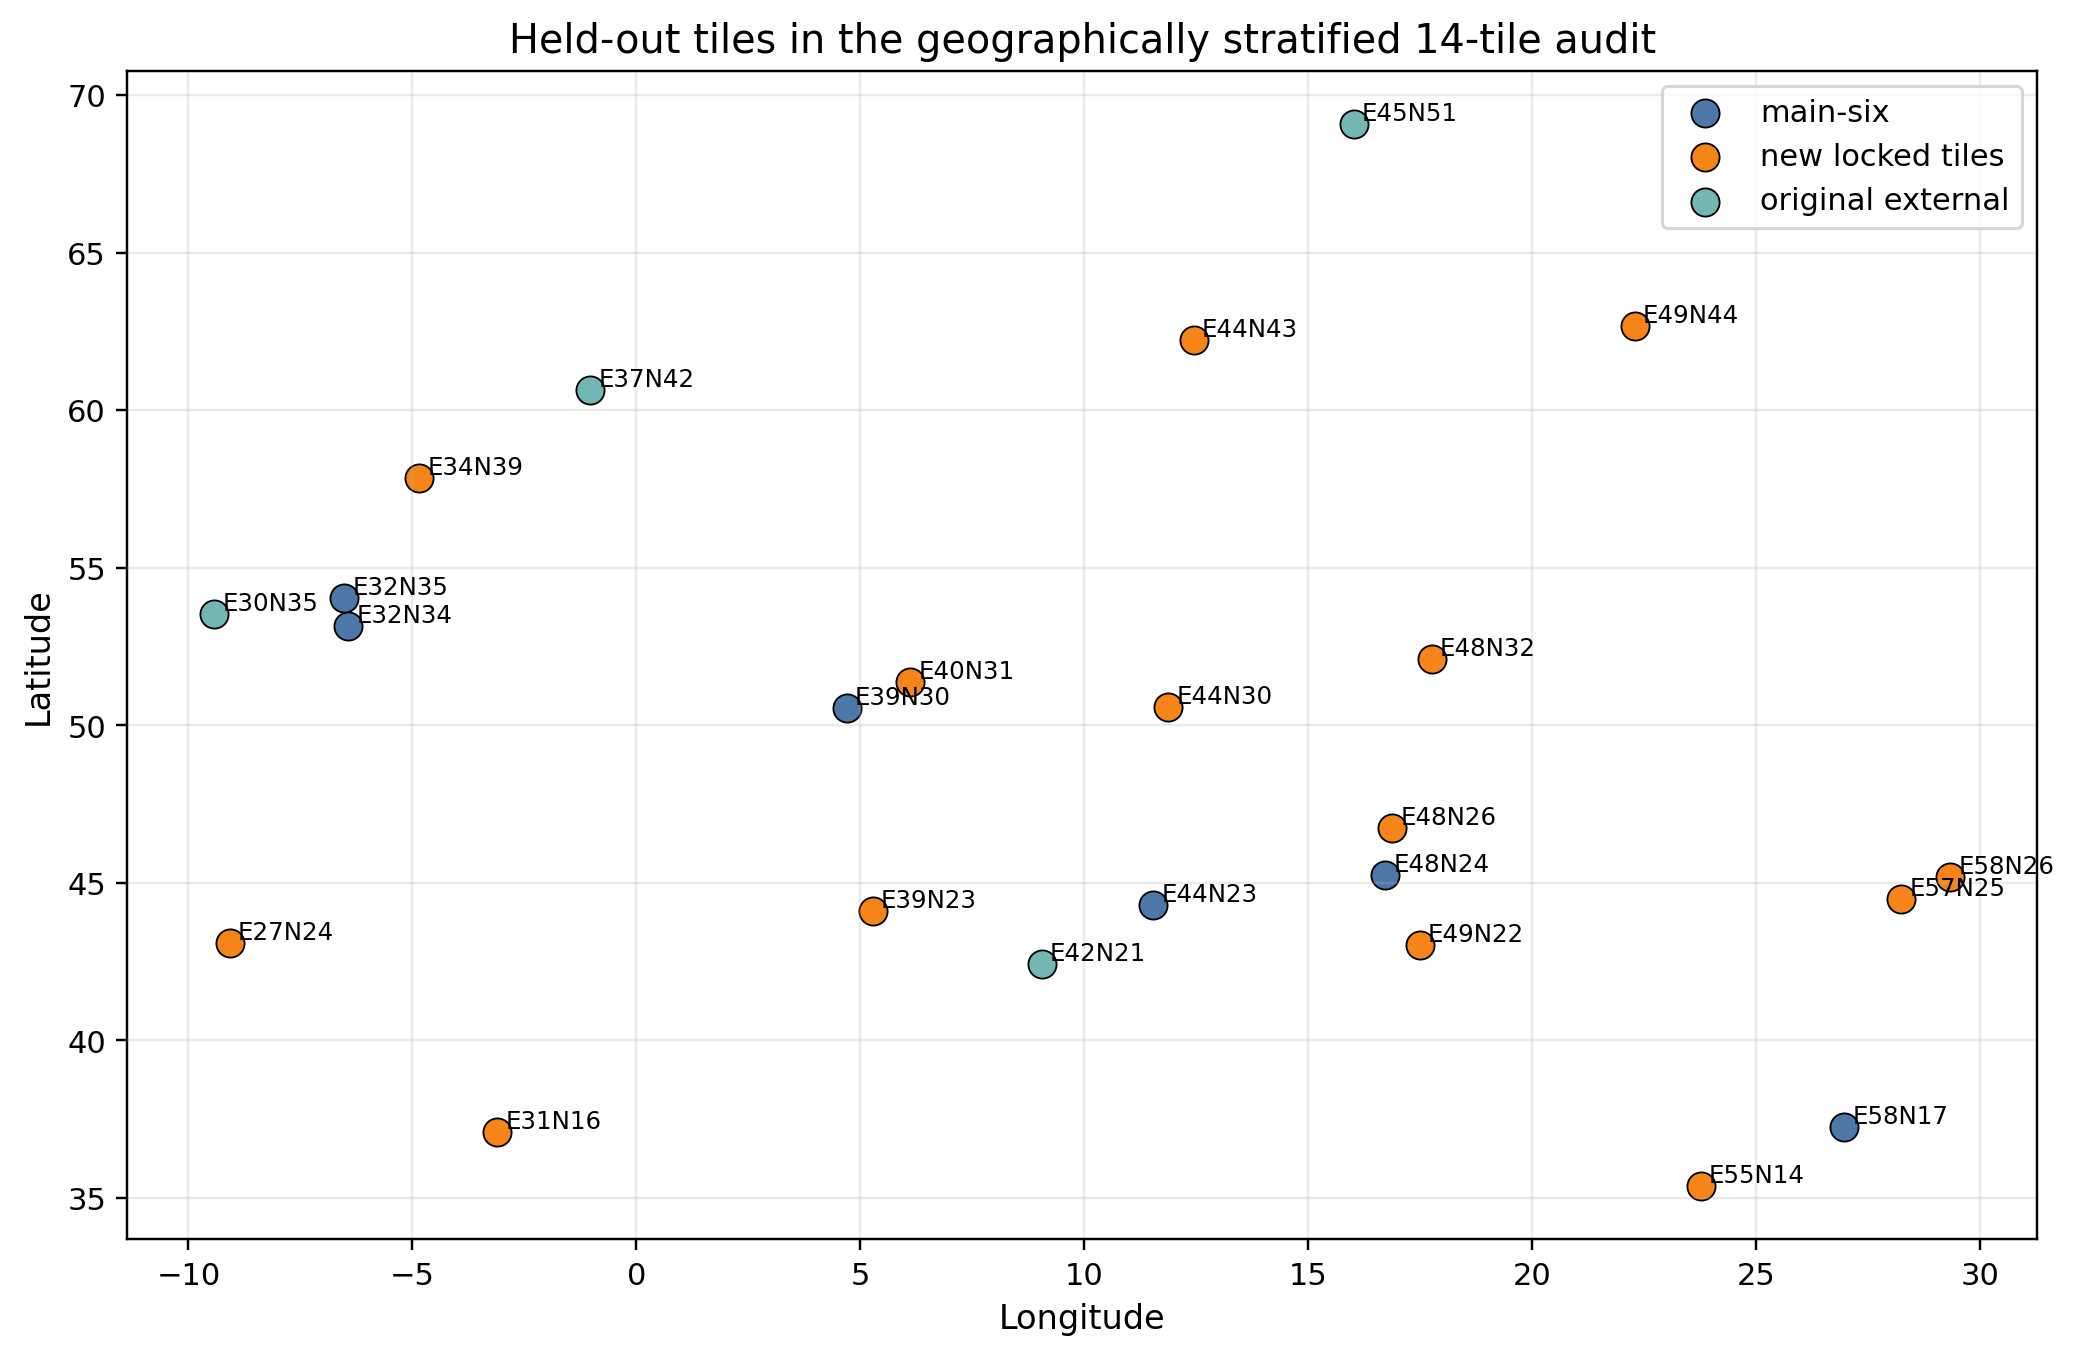
\includegraphics[width=0.95\textwidth]{paper_assets_vcea_extras/figures/E7_strong/fig_E7_pan_europe_tile_map.png}
\caption{Geographically stratified 14-tile European frozen audit design. The map shows the development tiles, the original external tiles, and the 14 held-out EGMS 2019--2023 tiles used in the audit. This is a finite metadata-stratified audit set rather than a population estimate over all European deformation conditions.}
\label{fig:e7_pan_europe_tile_map}
\end{figure*}

\begin{figure*}[!t]
\centering
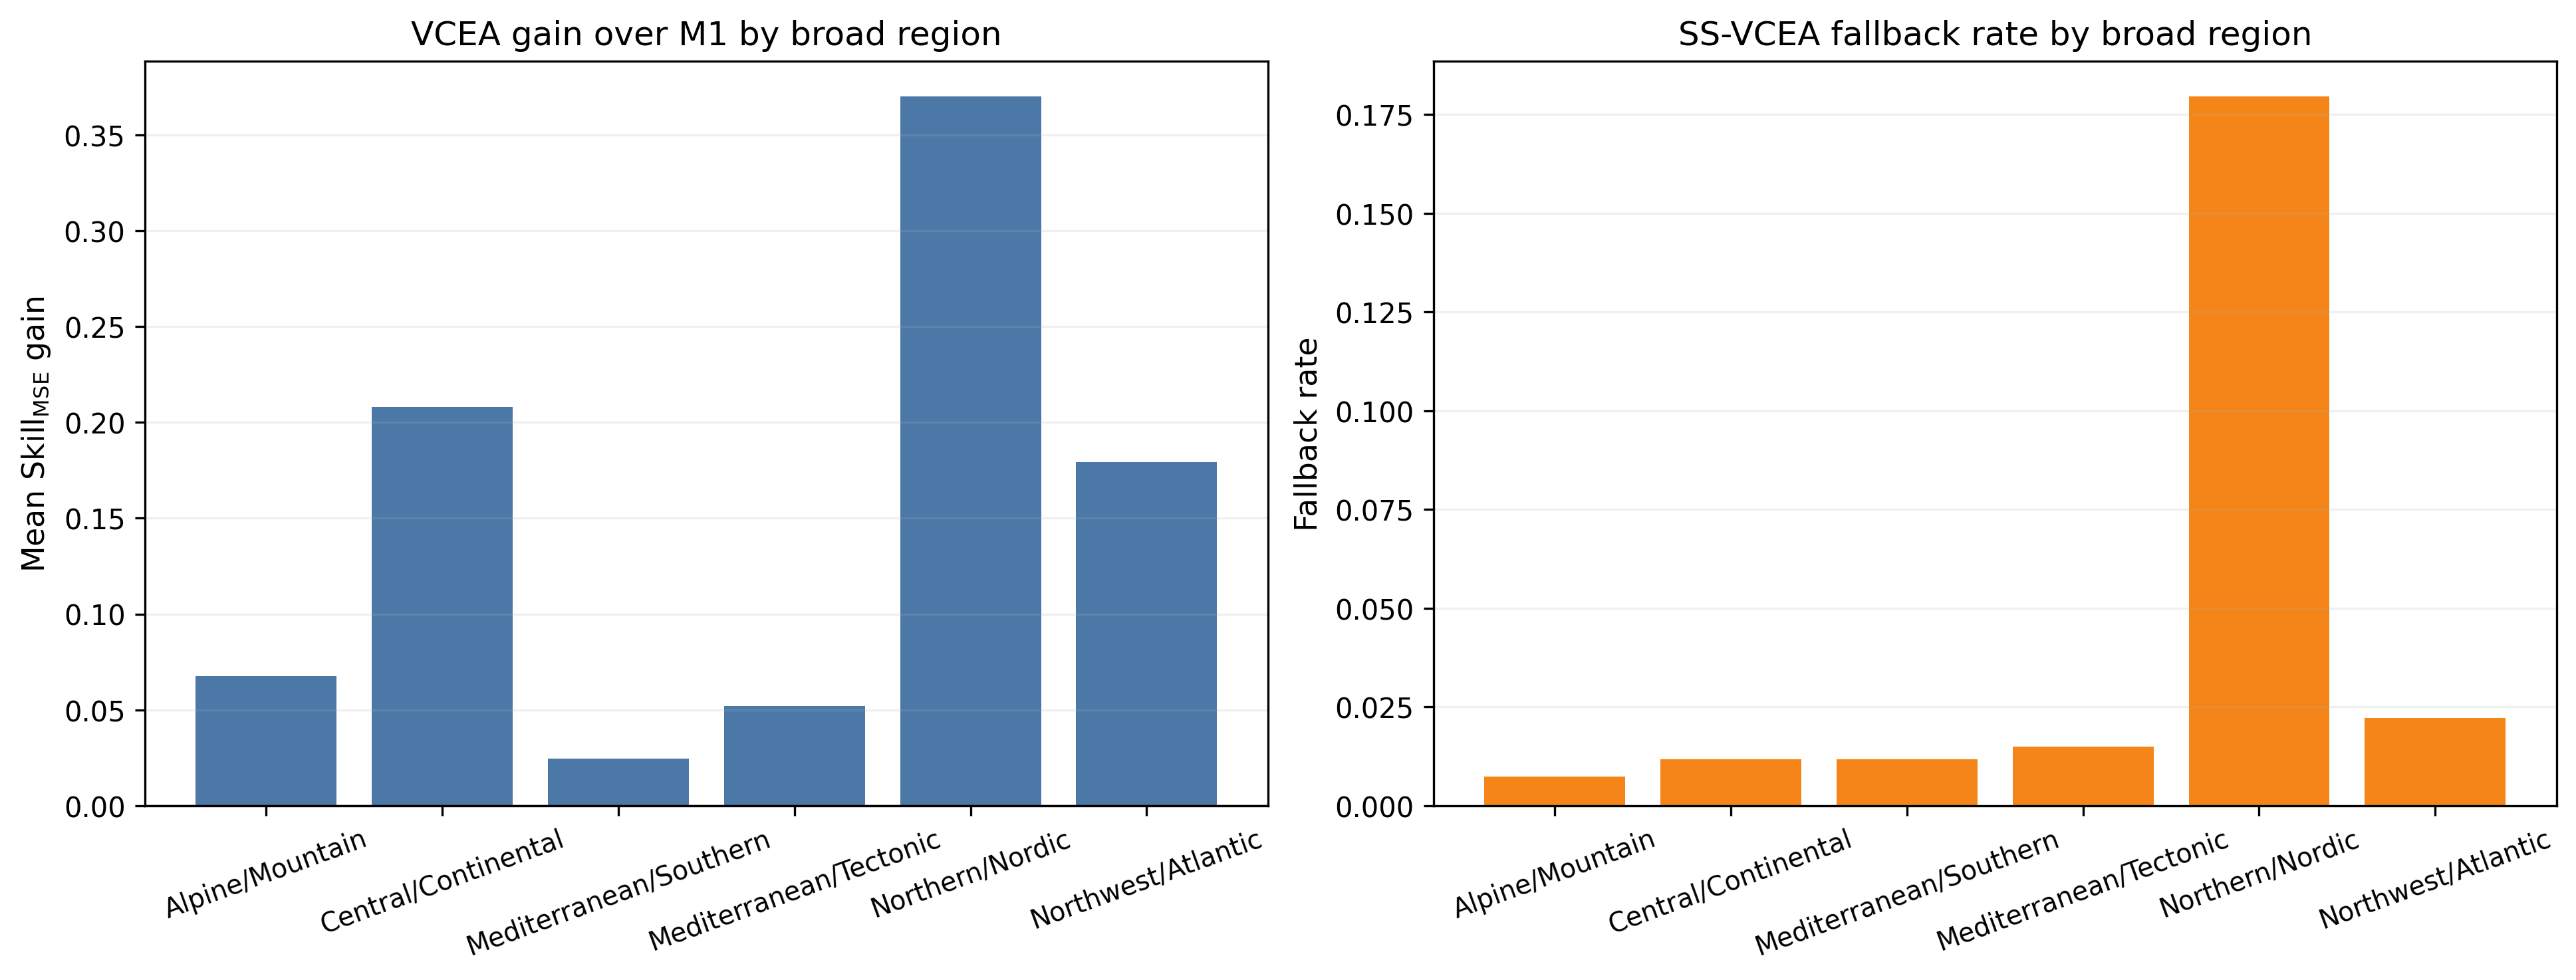
\includegraphics[width=0.95\textwidth]{paper_assets_vcea_extras/figures/E7_strong/fig_E7_skill_by_region.png}
\caption{Broad-region summary for the geographically stratified 14-tile European frozen audit. Over the 14 held-out tiles and 56 tile-horizon evaluations, VCEA supports positive average future-evaluation performance beyond the development and original external sets, while SS-VCEA preserves most of the gain with more conservative behavior.}
\label{fig:e7_skill_by_region}
\end{figure*}

\begin{figure*}[!t]
\centering
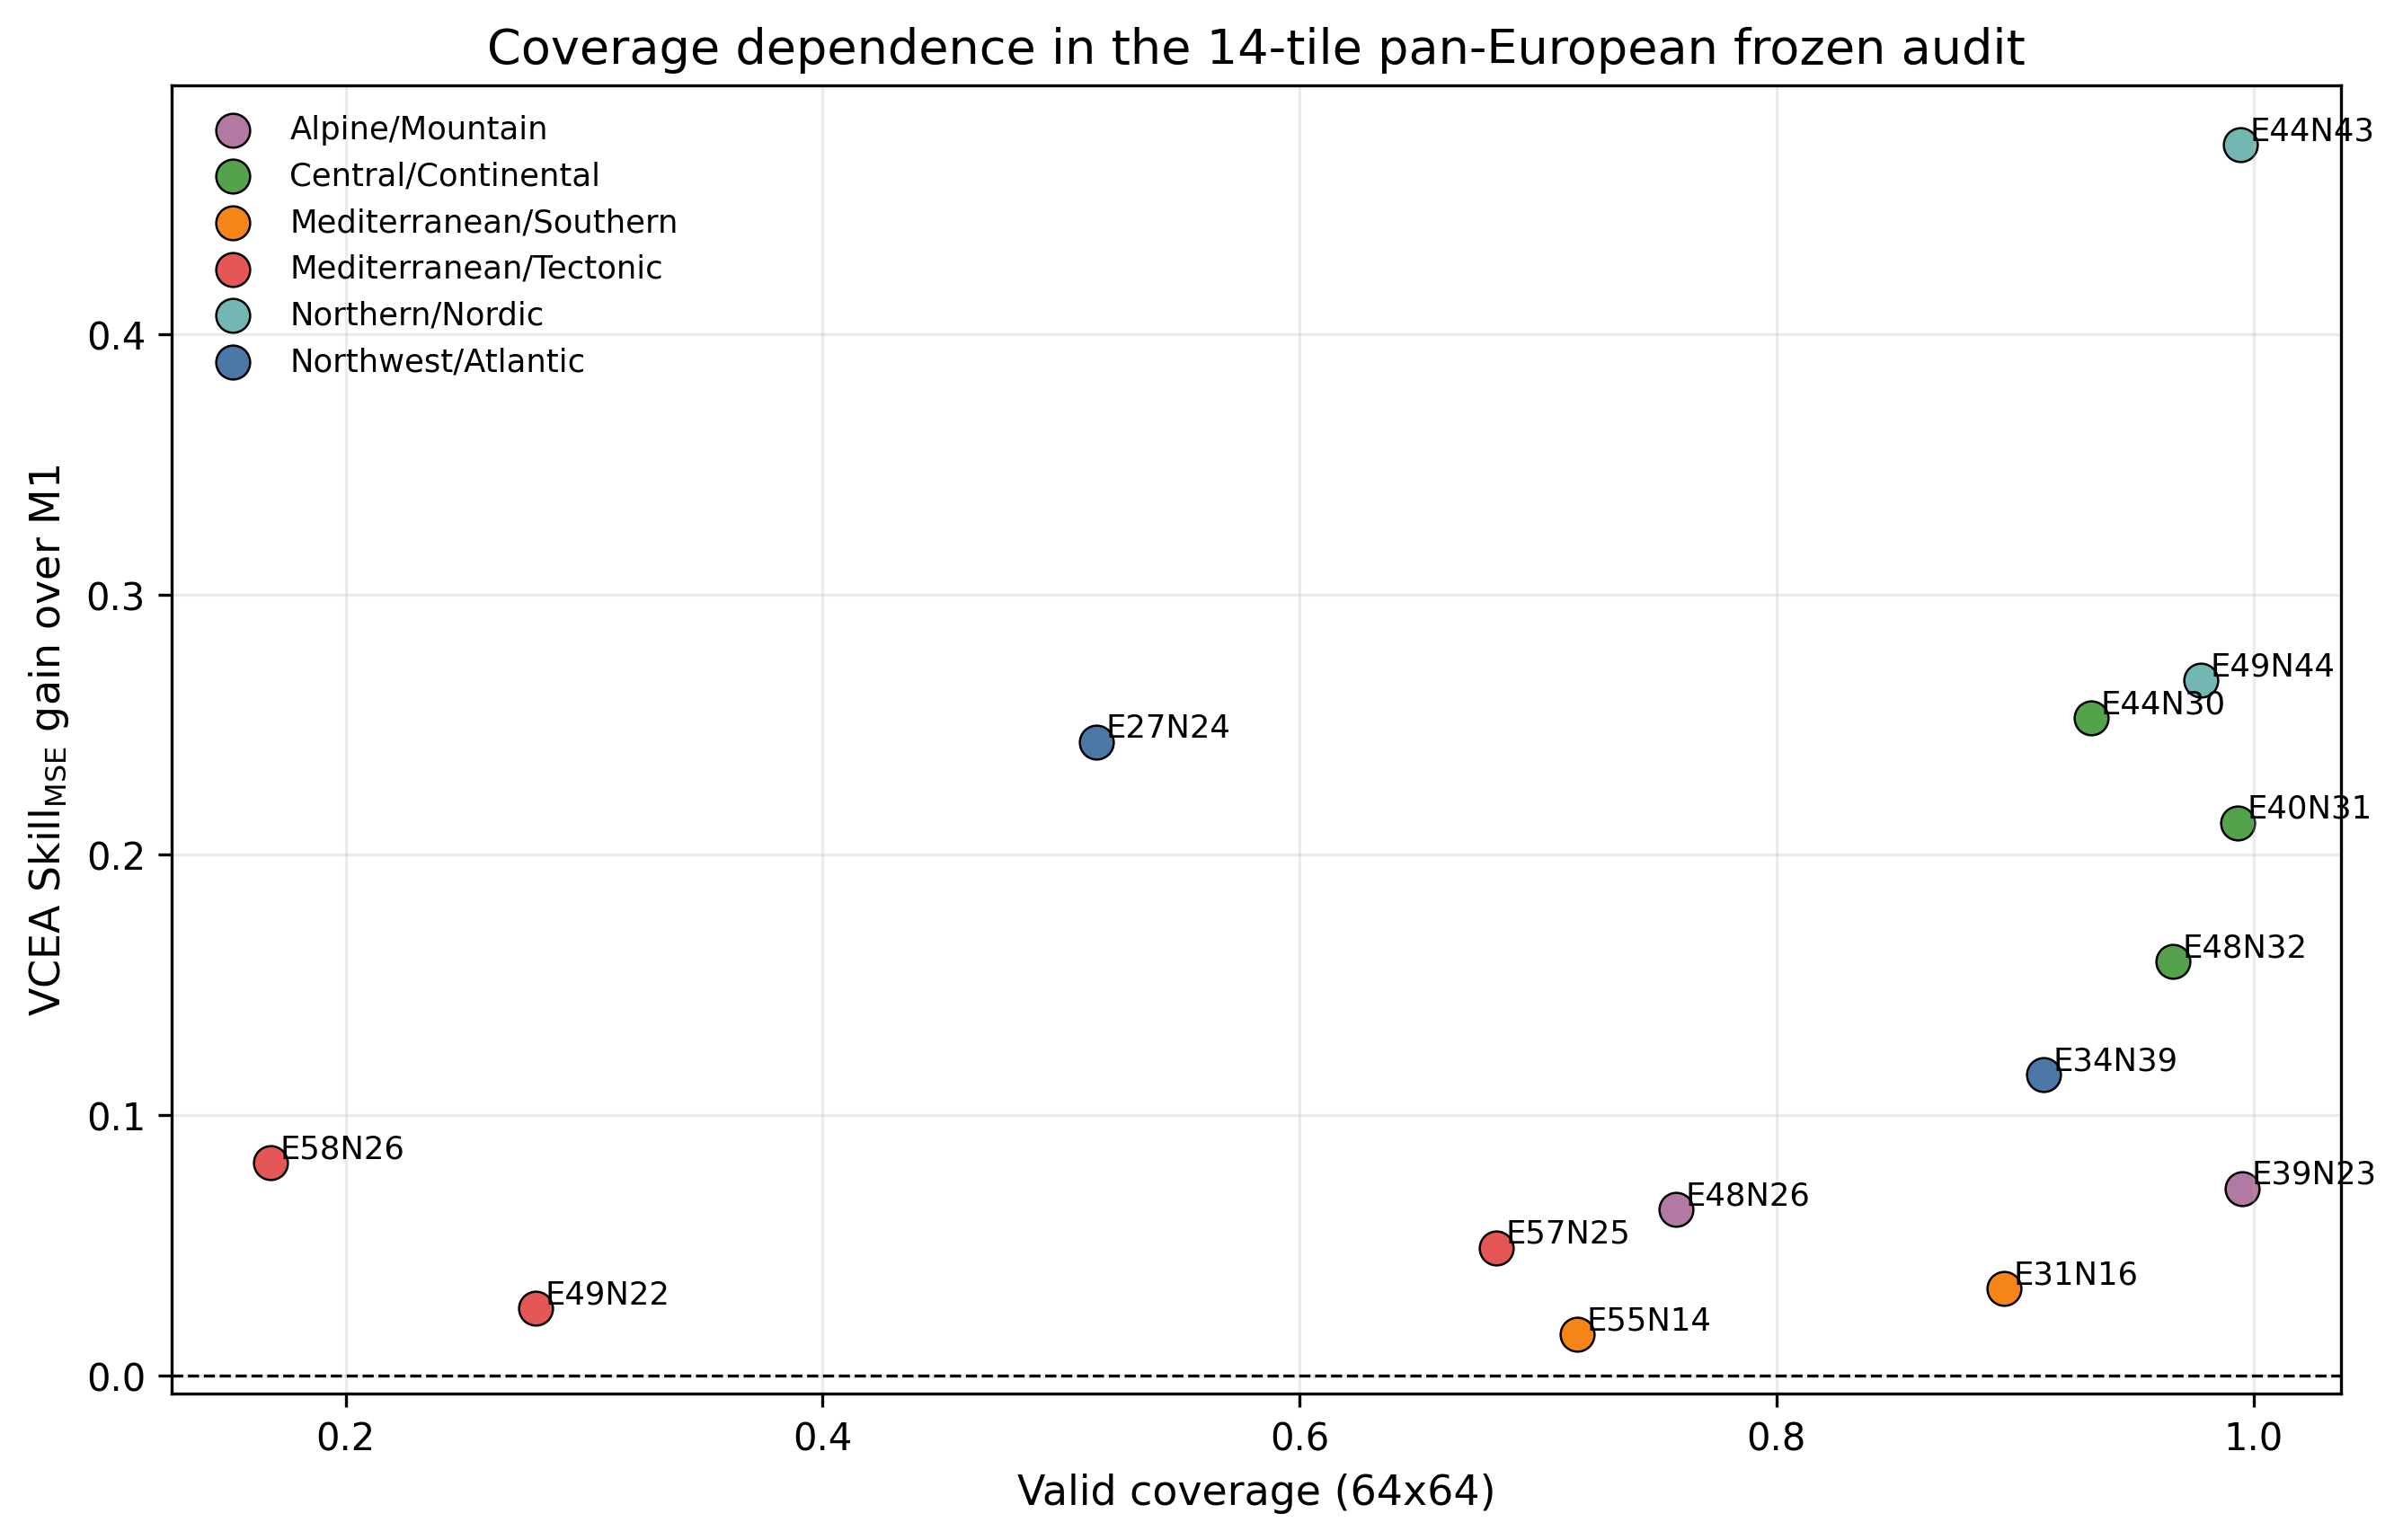
\includegraphics[width=0.95\textwidth]{paper_assets_vcea_extras/figures/E7_strong/fig_E7_skill_vs_coverage.png}
\caption{VCEA gain versus valid coverage in the geographically stratified 14-tile European frozen audit. The trend suggests that the future-evaluation gain is not reducible to a simple valid-coverage effect, although lower-support cases still define important limitations.}
\label{fig:e7_skill_vs_coverage}
\end{figure*}

Table~\ref{tab:e7_strong_failure_cases} lists localized operating-boundary cases. E44N43 has short temporal span, where VCEA is not better than M1 at $t{+}1$ and SS-VCEA has high fallback rates at $t{+}5$ and $t{+}10$. E49N22 is a low-coverage tile where VCEA is not better than M1 at $t{+}10$. These cases motivate future calibration work under limited history and sparse valid support.

\begin{table*}[!t]
\centering
\scriptsize
\begin{adjustbox}{max width=\textwidth}
\begin{tabular}{lllccccll}
\toprule
Tile & Horizon & Model & Skill$_{\mathrm{MSE}}$ & Gain vs M1 & Stress ratio & Fallback rate & Failure reason & Likely cause \\
\midrule
E44N43 & t+10 & SS-VCEA q97.5 & 0.524 & 0.172 & 0.690 & 0.514 & high fallback rate & short temporal span \\
E44N43 & t+5 & SS-VCEA q97.5 & 0.464 & 0.180 & 0.732 & 0.409 & high fallback rate & short temporal span \\
E44N43 & t+1 & VCEA & 0.113 & -0.031 & 0.942 & 0.009 & VCEA not better than M1 & short temporal span \\
E49N22 & t+10 & VCEA & 0.307 & -0.032 & 0.832 & 0.014 & VCEA not better than M1 & low coverage \\
\bottomrule
\end{tabular}
\end{adjustbox}
\caption{Operating-boundary cases in the geographically stratified 14-tile European frozen audit. Negative or high-fallback cases are localized, notably including short-temporal-span E44N43 cases and the low-coverage E49N22 case, rather than indicating a systematic failure of VCEA across held-out regions.}
\label{tab:e7_strong_failure_cases}
\end{table*}

\subsection{Sensitivity, Expert-Lineage, and Operational Diagnostics}
Resolution sensitivity indicates that the aggregation family is not merely exploiting a low-resolution artifact. M1 degrades as the grid is increased, while VCEA\_exact improves from 0.150 at $64\times64$ to 0.173 at $128\times128$ and 0.189 at $512\times512$. These values come from the resolution-aware sensitivity package and should not be read as replacements for the primary main-six claim of 0.178 in Table~\ref{tab:table06}. Because parts of the high-resolution package rely on proxy, transfer, or reused validation-cache assumptions, these results are sensitivity evidence rather than a replacement for the primary main-six benchmark.

The model-search audit further clarifies the role of neural experts. Preliminary model-search experiments evaluated robust neural baselines, stronger ACT-Former variants, selector families, online aggregation, static aggregation, STR-Mamba/KINO/CoMEx/RCDN candidates, and DSCF variants. Some candidates provided useful diagnostics or partial gains, but none displaced VCEA as the selected mainline configuration. Physics and regime diagnostics likewise show that gains are not uniform: subsidence and mixed regimes are more favorable for aggregation, while sparse coseismic tiles remain difficult. These diagnostics support the method's operating boundary as a regional map-updating tool rather than a physical event predictor. Full sensitivity, lineage, and diagnostic panels are provided in Appendices~\ref{app:safety_resolution} and~\ref{app:architecture_audit}.

\section{Discussion}
\subsection{Why Static Validation Calibration Works}
The key mechanism is validation-to-test stability under heterogeneous tile-horizon behavior. No single expert dominates all tiles and horizons: persistence anchors the short-horizon baseline, the linear-seasonal expert contributes explicit kinematic structure, and neural experts provide complementary residual correction. Tile- and horizon-aware calibration exploits this heterogeneity without using test labels. The expert-pool and calibration ablations show that this calibration is not optional: uniform averaging performs poorly on the main-six setting, while full validation-calibrated VCEA gives the best overall trade-off in this benchmark and the smallest oracle gap.

COEA remains useful because it demonstrates that aggregation is better than a single model and provides an online baseline. However, VTSA, blocked-validation analysis, and weight-drift diagnostics explain why online adaptation is not the dominant ingredient in this benchmark. When validation expert rankings remain informative for the test period, a static validation mixture can outperform delayed-feedback online updates.

\subsection{Why Complex Single Models Were Not Enough}
The best-performing single model in the evaluated pool, M1/C2, establishes that neural residual correction is useful, but its mean \skillmse{} remains far below VCEA. More complex candidates often overcorrect, fail to generalize across tiles, or produce insufficient incremental value over the aggregation family. This does not imply that neural models are unnecessary; rather, they are most effective here as experts inside a strong-baseline-aware mixture.

\subsection{From Original External Evaluation to the 14-Tile European Frozen Audit}
The original four-tile external locked evaluation provided an initial held-out future-evaluation check under tile-local historical validation calibration, and the geographically stratified 14-tile European frozen audit expands this evidence to 14 held-out EGMS 2019--2023 tiles under the same protocol family. The audit shows positive future-evaluation performance across the tested broad-region strata, audit-regime groups, and coverage groups, with VCEA improving over M1 on all 14 held-out tiles and SS-VCEA preserving most of the gain with stress ratio below one.

This evidence remains deliberately bounded. EGMS is a continental service, but the audit set is finite and metadata-stratified rather than a census of all deformation conditions. The correct interpretation is positive future-evaluation performance across the tested held-out EGMS tiles and groups, not a Europe-wide population claim.

\subsection{Regional Screening and Operational Boundaries}
The benchmark is designed for regional screening and map updating. The $64\times64$ main task is intentionally coarse, and the 128/512 experiments are sensitivity checks rather than claims of native-resolution operational use. Likewise, coseismic analyses are interpreted as post-event realignment and diagnostic behavior, not as earthquake occurrence prediction.
Stress reduction in SS-VCEA should therefore be interpreted as reduced forecasting over-correction pressure rather than reduced physical deformation risk.

\subsection{Operating Boundaries and Limitations}
The main localized operating-boundary cases in the geographically stratified 14-tile European frozen audit are associated with short temporal span and low coverage. On E44N43, VCEA is not better than M1 at $t{+}1$, and SS-VCEA has high fallback rates at $t{+}5$ and $t{+}10$, consistent with limited temporal history. On E49N22, VCEA is not better than M1 at $t{+}10$, consistent with low valid-cell coverage and sparse support. Future work should therefore focus on calibration under short temporal span, sparse support, low valid coverage, and broader deformation regimes.

Additional limitations remain. Some high-resolution sensitivity results involve proxy, transfer, or cache-reuse assumptions. The SS-VCEA risk score uses an equal-normalized design choice from the matched operating-point reference study and should be revisited if domain-specific risk weights become available. Finally, while the workflow is leakage-safe and audit-driven, the method is not a physics-informed simulator.

\section{Reproducibility Statement}
The reproducibility package records product manifests, tile manifests, split definitions, expert cache provenance, aggregation calibration, threshold diagnostics, 14-tile audit metadata, software environment details, main random seeds, and exact/proxy/transfer flags where relevant. These materials make it possible to trace each manuscript claim to the corresponding data split, expert cache, threshold choice, and result table. A compact claim-to-evidence map and the detailed asset traceability tables are provided in Appendix~\ref{app:repro_trace}.

\section{Conclusion}
We formulate EGMS regional ground-deformation nowcasting as validation-calibrated expert aggregation under strong persistence baselines. Within this formulation, VCEA uses validation-only tile- and horizon-aware static weights and improves over the best-performing single-model baseline among the evaluated candidates on the primary main-six benchmark. The same frozen framework also shows positive future-evaluation performance on the geographically stratified 14-tile European frozen audit of held-out EGMS tiles under tile-local historical validation calibration.

SS-VCEA q97.5 provides a conservative operating point with reduced stress under the tested protocols. The remaining operating-boundary cases are localized to short temporal span and low valid coverage, suggesting that future work should extend calibration under limited history, sparse valid support, and broader deformation regimes.
\ifusebibtexrefs
\bibliographystyle{IEEEtran}
\bibliography{ref}
\fi

\clearpage
\onecolumn
\appendices

\section{Additional Protocol and Metric Details}
\label{app:protocol_metric_details}
The appendix is provided as supplementary material within the same PDF. It contains extended audit tables, statistical robustness checks, reproducibility manifests, and claim-to-evidence mappings supporting the main text.

This appendix gathers protocol, metric, and expert-pool details that support the main text but would otherwise overload the main narrative.

\begin{figure}[!t]
  \centering
  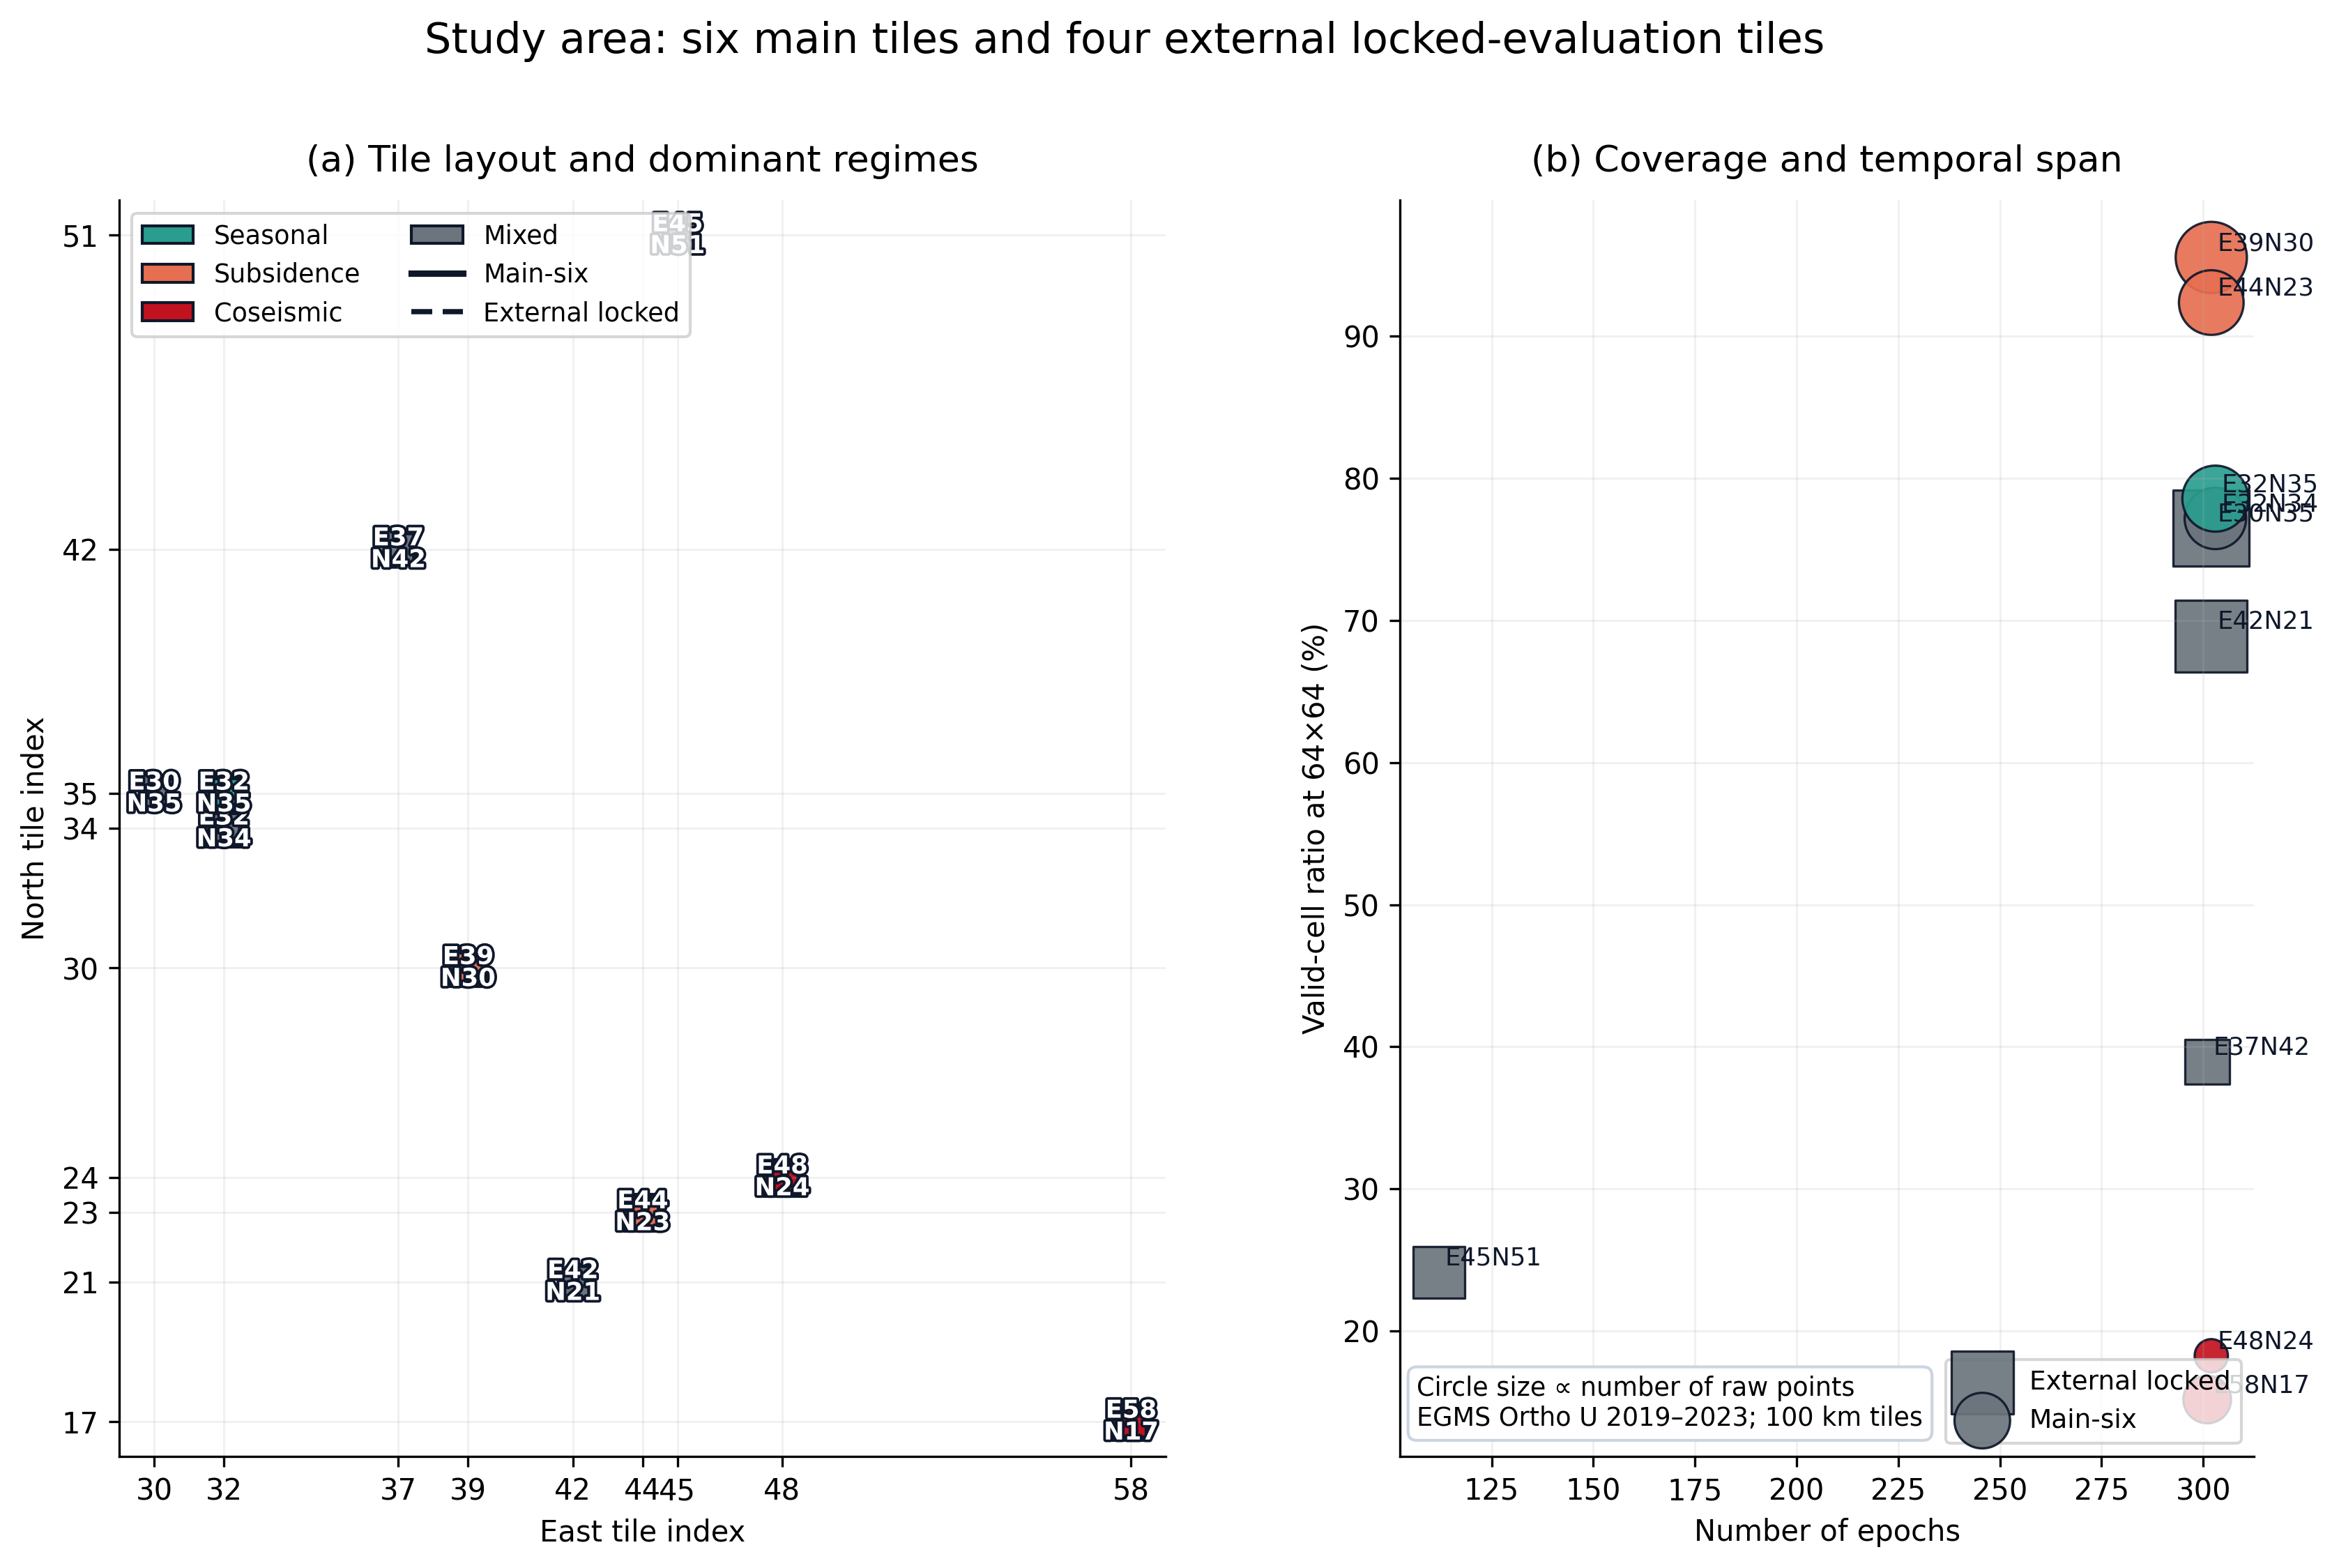
\includegraphics[width=0.95\textwidth]{figures/final/Fig01_study_area_map.png}
  \caption{Study area and coverage of the unified EGMS 2019--2023 Ortho U benchmark. (a) The six main-development tiles and four original external locked-evaluation tiles are shown with their dominant regime labels. (b) Temporal span and valid-cell coverage at the primary $64\times64$ setting. Main-six tiles were used for model development, whereas the original external tiles remained frozen for locked evaluation.}
  \label{fig:fig01}
\end{figure}

\begin{table}[!t]
  \centering
  \caption{Metadata of the six main-development tiles and four original external locked-evaluation tiles, including dominant regime labels, temporal span, valid-cell coverage, and raw point counts.}
  \label{tab:table01}
  \scriptsize
  \begin{adjustbox}{max width=\textwidth}
  \begin{tabular}{lllp{0.16\textwidth}rrrr}
    \toprule
    Tile & Group & Role & \shortstack{Dominant\\regime} & Frames & Valid64 & Valid128 & \shortstack{Num\\points} \\
    \midrule
    E32N34 & main6 & source\_main & mixed & 303 & 0.772 & 0.698 & 138926 \\
    E32N35 & main6 & nearby\_seasonal & seasonal & 303 & 0.786 & 0.756 & 185125 \\
    E39N30 & main6 & subsidence\_1 & subsidence & 302 & 0.955 & 0.807 & 250830 \\
    E44N23 & main6 & subsidence\_2 & subsidence & 302 & 0.924 & 0.780 & 170553 \\
    E48N24 & main6 & coseismic\_1 & coseismic & 302 & 0.183 & 0.106 & 11911 \\
    E58N17 & main6 & coseismic\_2 & coseismic & 301 & 0.152 & 0.126 & 50260 \\
    E37N42 & external\_locked & external & mixed & 301 & 0.389 & 0.338 & 39626 \\
    E45N51 & external\_locked & external & mixed & 112 & 0.241 & 0.199 & 69604 \\
    E30N35 & external\_locked & external & mixed & 302 & 0.765 & 0.726 & 323481 \\
    E42N21 & external\_locked & external & mixed & 302 & 0.689 & 0.633 & 261823 \\
    \bottomrule
  \end{tabular}
  \end{adjustbox}
\end{table}

\begin{table}[!t]
  \centering
  \caption{Definitions of the primary accuracy, operational-control, robustness, diagnostic, and reproducibility metrics used in the study.}
  \label{tab:table03}
  \footnotesize
  \begin{adjustbox}{max width=\textwidth}
  \begin{tabular}{p{0.17\textwidth}p{0.21\textwidth}p{0.50\textwidth}}
    \toprule
    \shortstack{Metric\\group} & Metric & Purpose \\
    \midrule
    Accuracy & RMSE & Primary magnitude error \\
    Accuracy & MAE & Robust average absolute error \\
    Accuracy & Skill$_{\mathrm{MSE}}$ & $1 - \mathrm{MSE}_{\mathrm{model}} / \mathrm{MSE}_{\mathrm{persistence}}$ \\
    Accuracy & Skill$_{\mathrm{RMSE}}$ & Relative RMSE improvement over persistence \\
    Accuracy & Acc@1mm / Acc@0.5mm & Thresholded accuracy \\
    Accuracy & SSIM & Structural similarity \\
    Operational control & stress ratio & Operational over-correction and reliability indicator relative to persistence; not a geophysical hazard metric \\
    Operational control & fallback rate & Fraction of conservative fallback in SS-VCEA \\
    Operational control & correction magnitude & Magnitude of residual correction / operational risk \\
    Robustness & better tiles & How many tiles outperform the baseline \\
    Robustness & seed std & Stability across random seeds \\
    Robustness & external locked gain & Generalization beyond the main-six benchmark \\
    Diagnostics & velocity-sign consistency & Sign consistency on moving pixels \\
    Diagnostics & jump rate & Unrealistic temporal jump frequency \\
    Diagnostics & post-event recovery ratio & Post-event stabilization diagnostic \\
    Diagnostics & regime-wise metrics & Stable/seasonal/subsidence/accelerating/coseismic/mixed diagnostics \\
    Efficiency/Repro & train time / inference time / peak memory & Engineering cost \\
    Efficiency/Repro & lineage / exact-proxy-transfer flags & Reproducibility provenance \\
    \bottomrule
  \end{tabular}
  \end{adjustbox}
\end{table}

\begin{table}[!t]
  \centering
  \caption{Summary of evaluated experts and baselines. VCEA and SS-VCEA operate above this fixed pool rather than introducing a new backbone architecture.}
  \label{tab:table04}
  \footnotesize
  \begin{adjustbox}{max width=\textwidth}
  \begin{tabular}{p{0.12\textwidth}p{0.13\textwidth}p{0.13\textwidth}p{0.17\textwidth}p{0.16\textwidth}cp{0.17\textwidth}}
    \toprule
    Name & Role & \shortstack{Model\\family} & \shortstack{Input /\\update mode} & \shortstack{Training or\\calibration source} & \shortstack{Used by\\VCEA?} & Notes \\
    \midrule
    Persistence & reference baseline & persistence map & Last available EGMS displacement map & No training & Yes & Strong short-horizon reference and skill denominator \\
    Linear-Seasonal & kinematic expert & seasonal/trend extrapolation & Tile-wise parametric extrapolation & Per-tile historical fit & Yes & Weak standalone baseline but useful inside calibrated mixtures \\
    M1 / C2 & robust neural expert & residual-query ACT line & Offline neural prediction from 16-frame history & Full-six exact training & Yes & Best-performing single-model baseline among evaluated candidates \\
    C3\_opt & complementary neural expert & higher-capacity state-mixer line & Offline neural prediction from 16-frame history & Full-six exact training & Yes & Retained for complementarity rather than as the final standalone model \\
    COEA & online comparison expert & delayed-feedback aggregation & Sequential online update after target observability & Validation warm start + delayed-feedback updates & No & Uses labels only after the corresponding targets become observable \\
    VCEA & calibrated aggregate & static expert aggregation & Tile$\times$horizon static weighted mixture & Tile-local historical validation calibration & --- & Main validation-calibrated aggregation method \\
    SS-VCEA q97.5 & conservative fallback variant & VCEA + fallback control & VCEA output with validation-calibrated hard fallback & VCEA weights + pooled main-six validation thresholds & --- & Conservative operating variant using the COEA fallback branch \\
    \bottomrule
  \end{tabular}
  \end{adjustbox}
\end{table}

\begin{table}[!t]
  \centering
  \caption{Protocol comparison between VCEA, COEA, and SS-VCEA, emphasizing weight source, update mode, fallback control, and whether any test-time tuning is allowed.}
  \label{tab:table05}
  \footnotesize
  \begin{adjustbox}{max width=\textwidth}
  \begin{tabular}{p{0.11\textwidth}p{0.18\textwidth}p{0.16\textwidth}p{0.18\textwidth}cp{0.20\textwidth}}
    \toprule
    Method & \shortstack{Weight\\source} & \shortstack{Update\\mode} & \shortstack{Fallback\\control} & \shortstack{Test\\tuning} & Role \\
    \midrule
    VCEA & Validation-only static calibration & Tile$\times$horizon static weights & -- & No & Best-accuracy mainline \\
    COEA & Validation warm start + online update & Delayed-feedback online update & -- & No & Online aggregation baseline \\
    SS-VCEA & Reuse VCEA + validation-calibrated threshold & Static VCEA output & Risk-triggered hard fallback & No & Conservative operating variant \\
    \bottomrule
  \end{tabular}
  \end{adjustbox}
\end{table}

\subsection{Full Versions of the Main Audit Tables}
\label{app:e1_e3_full_tables}
For compactness, the main text uses shortened versions of the split-protocol, expert-pool, and calibration tables. Their full manuscript versions are reproduced here without changing any numerical values.

\begin{table}[!t]
\centering
\scriptsize
\begin{adjustbox}{max width=\textwidth}
\begin{tabular}{llrrrrrrrp{0.14\textwidth}}
\toprule
Protocol & Window rule & Train windows & Val windows & Test windows & VCEA Skill$_{\mathrm{MSE}}$ & M1 Skill$_{\mathrm{MSE}}$ & VCEA gain vs M1 & SS-VCEA stress ratio & Conclusion \\
\midrule
Target-time assignment & Target assigned to split; history may cross boundary without future target access & 1117 & 120 & 306 & 0.178 & 0.078 & 0.099 & 0.992 & positive gain retained \\
Full-window containment & History window and all target horizons must remain in the same split & 1117 & 30 & 216 & 0.159 & 0.080 & 0.079 & 1.152 & positive gain retained \\
Gap-buffer (10 frames) & Ten-frame buffer inserted after split boundaries before target windows begin & 1057 & 60 & 246 & 0.170 & 0.085 & 0.085 & 1.133 & positive gain retained \\
\bottomrule
\end{tabular}
\end{adjustbox}
\caption{Full split-protocol audit table corresponding to the compact main-text version in Table~\ref{tab:e1_leakage_audit}.}
\label{tab:e1_leakage_audit_full}
\end{table}

\begin{table}[!t]
\centering
\footnotesize
\begin{adjustbox}{max width=\textwidth}
\begin{tabular}{llrrrrp{0.20\textwidth}}
\toprule
Variant & Expert pool & Main-six Skill$_{\mathrm{MSE}}$ & External Skill$_{\mathrm{MSE}}$ & Stress ratio & Better tiles & Interpretation \\
\midrule
VCEA\_full & Persistence, Linear-Seasonal, M1, C3\_opt & 0.178 & 0.317 & 1.046 & 6 & full pool reference \\
without\_persistence & Linear-Seasonal, M1, C3\_opt & 0.176 & 0.334 & 1.088 & 5 & ablation / diagnostic \\
without\_C3\_opt & Persistence, Linear-Seasonal, M1 & 0.158 & 0.323 & 1.093 & 5 & ablation / diagnostic \\
without\_M1 & Persistence, Linear-Seasonal, C3\_opt & 0.155 & 0.307 & 1.082 & 4 & ablation / diagnostic \\
only\_neural & M1, C3\_opt & 0.127 & 0.192 & 0.995 & 6 & ablation / diagnostic \\
without\_linear\_seasonal & Persistence, M1, C3\_opt & 0.112 & 0.174 & 0.996 & 5 & ablation / diagnostic \\
only\_kinematic & Persistence, Linear-Seasonal & 0.091 & 0.300 & 1.196 & 3 & ablation / diagnostic \\
uniform\_expert\_average & Persistence, Linear-Seasonal, M1, C3\_opt & -1.805 & 0.267 & 4.112 & 3 & ablation / diagnostic \\
\bottomrule
\end{tabular}
\end{adjustbox}
\caption{Full expert-pool ablation table corresponding to the compact main-text version in Table~\ref{tab:e2_expert_ablation_main6}.}
\label{tab:e2_expert_ablation_main6_full}
\end{table}

\begin{table}[!t]
\centering
\footnotesize
\begin{adjustbox}{max width=\textwidth}
\begin{tabular}{lcccrrrr}
\toprule
Aggregation & Calibration source & Tile-aware & Horizon-aware & Main-six Skill$_{\mathrm{MSE}}$ & External Skill$_{\mathrm{MSE}}$ & Stress ratio & Oracle gap \\
\midrule
Uniform average & uniform & 0 & 0 & -1.805 & 0.267 & 4.112 & 2.002 \\
Global validation weights & validation & 0 & 0 & 0.129 & 0.281 & 1.051 & 0.067 \\
Tile-only VCEA & validation & 1 & 0 & 0.154 & 0.255 & 1.046 & 0.042 \\
Horizon-only VCEA & validation & 0 & 1 & 0.133 & 0.320 & 1.047 & 0.063 \\
Full tile+horizon VCEA & validation & 1 & 1 & 0.178 & 0.317 & 1.046 & 0.019 \\
Oracle test weights & test-oracle & 1 & 1 & 0.196 & 0.356 & 0.996 & 0.000 \\
\bottomrule
\end{tabular}
\end{adjustbox}
\caption{Full calibration ablation table corresponding to the compact main-text version in Table~\ref{tab:e3_calibration_ablation}.}
\label{tab:e3_calibration_ablation_full}
\end{table}

\begin{figure}[!t]
  \centering
  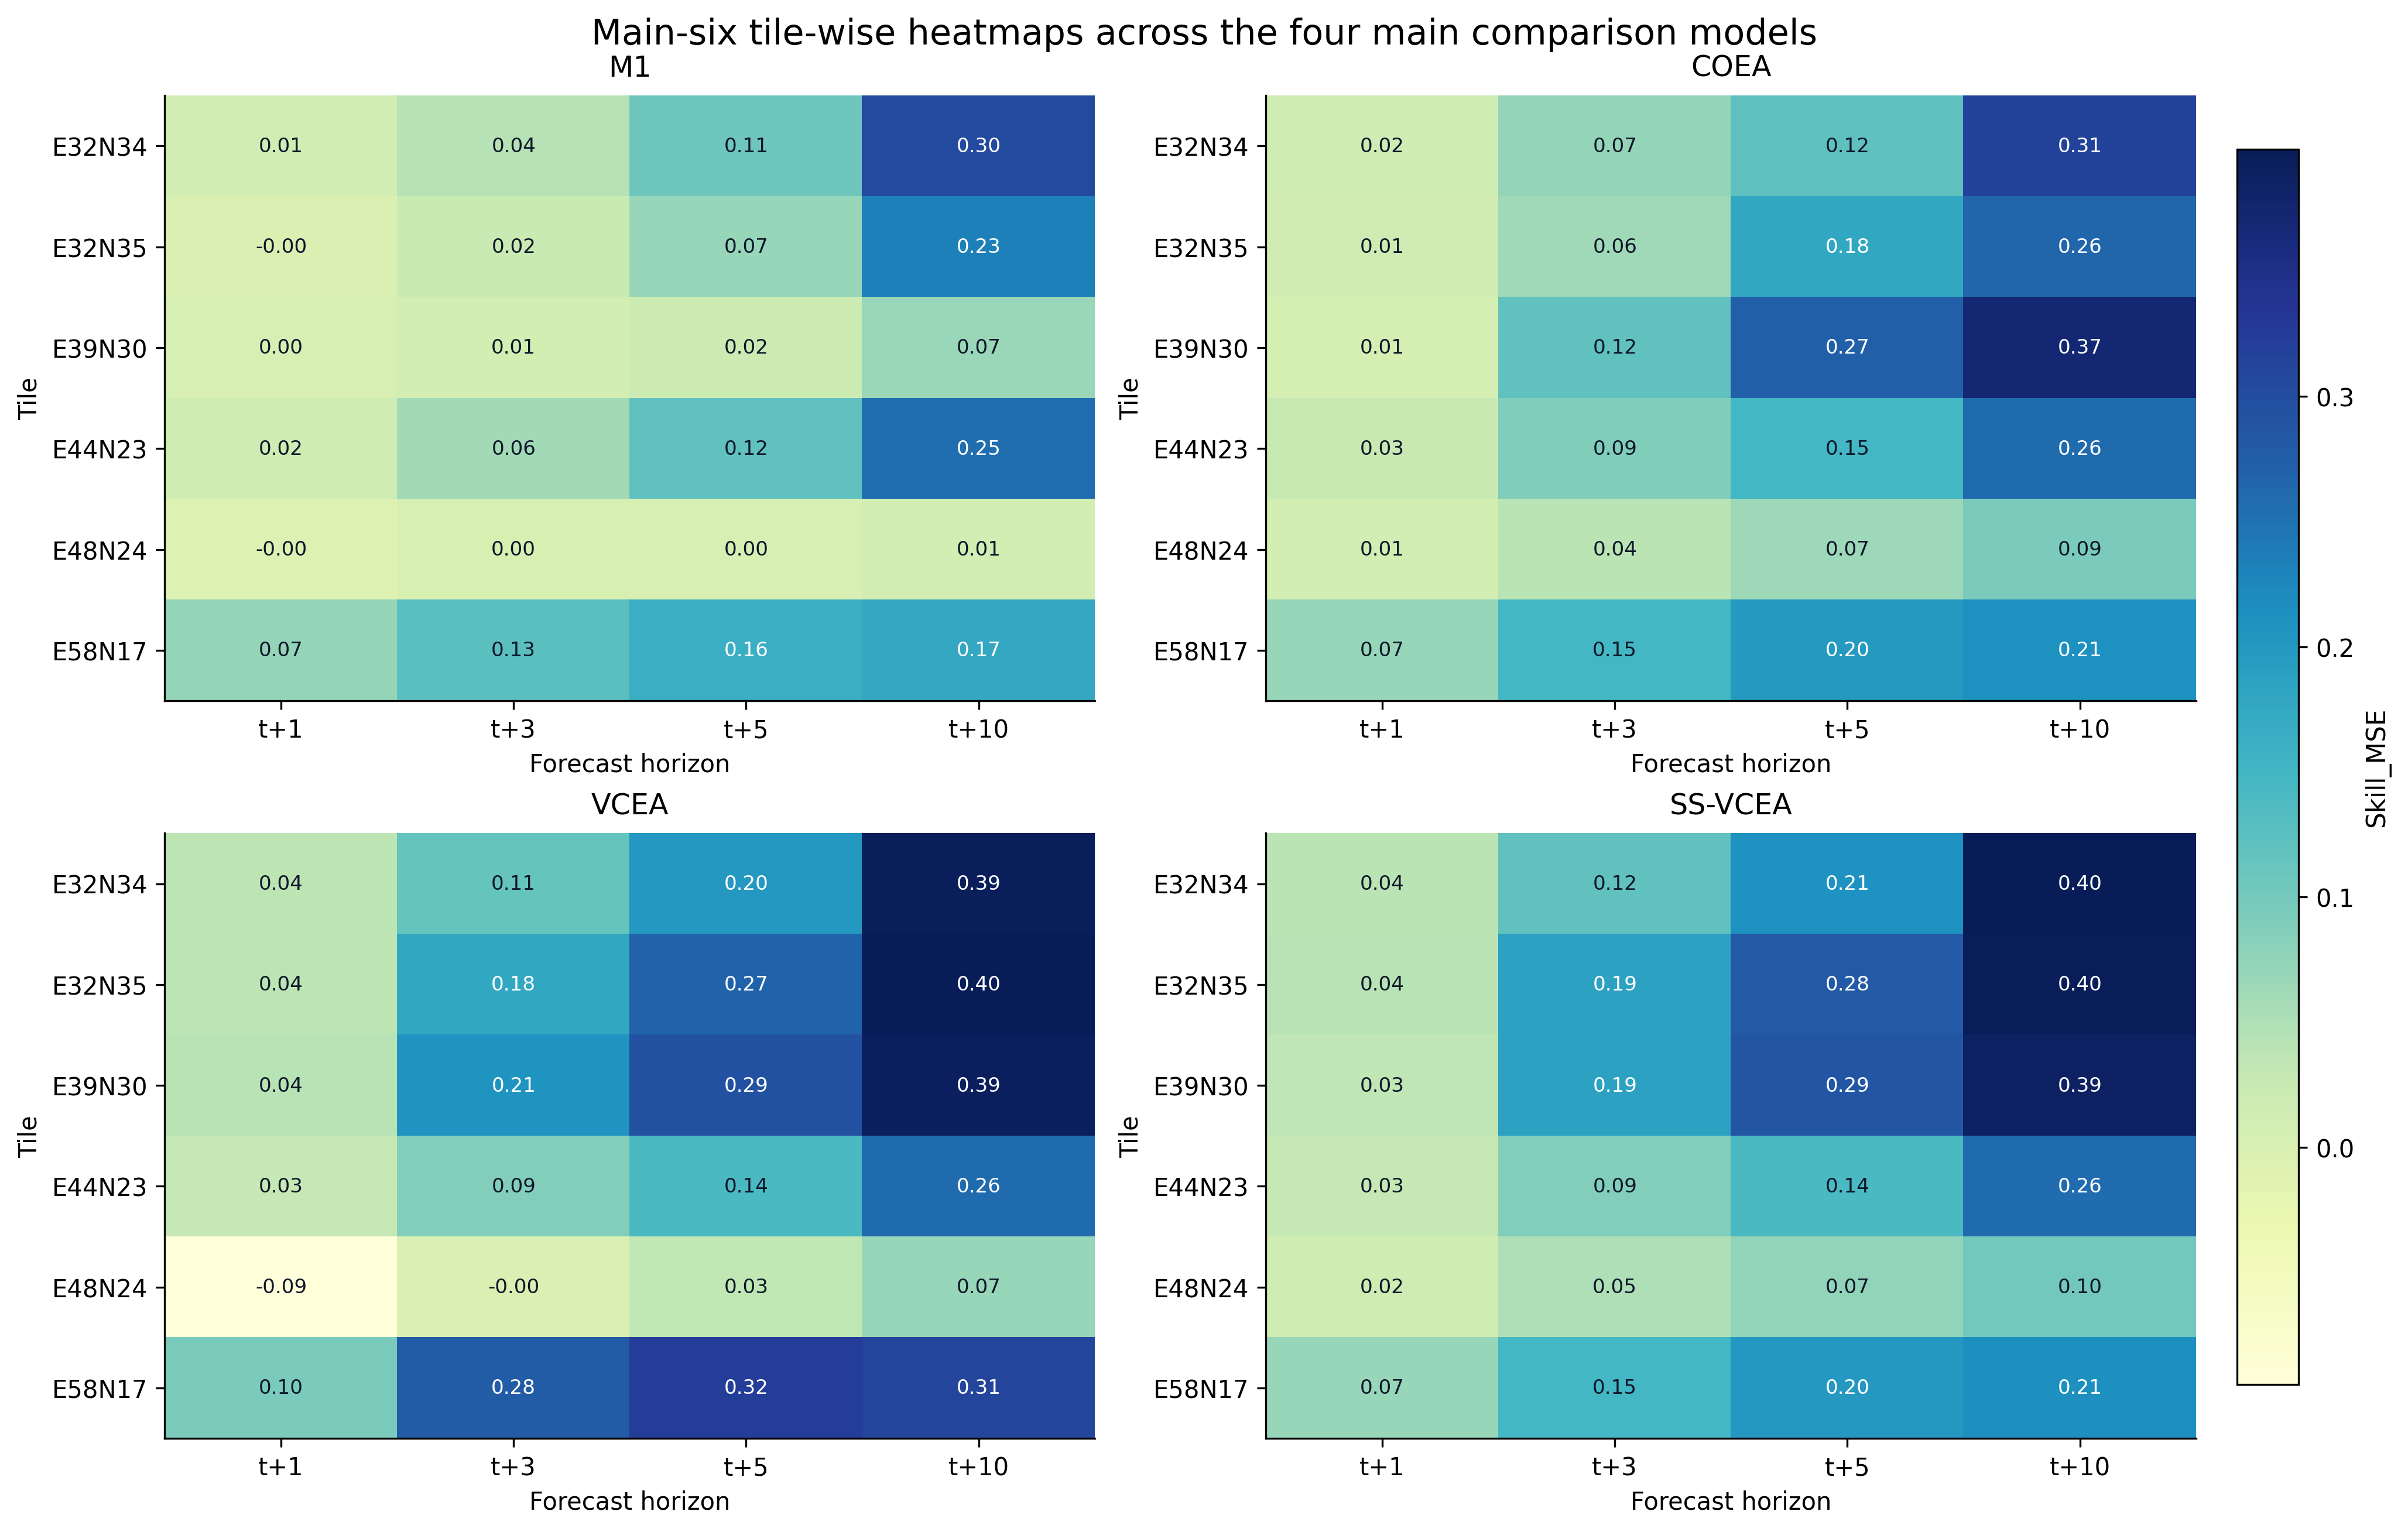
\includegraphics[width=0.95\textwidth]{figures/final/Fig06_main_six_tile_heatmap_panel.png}
  \caption{Main-six tile-wise heatmaps for the four primary comparison models: M1, COEA, VCEA, and the selected SS-VCEA operating variant. Each cell reports mean \skillmse{} for one tile-horizon pair. The panel highlights that aggregation gains are spatially heterogeneous, while SS-VCEA largely preserves the tile-wise benefits of VCEA.}
  \label{fig:fig06}
\end{figure}

\section{Blocked-Validation and Validation-Transfer Diagnostics}
\label{app:blocked_validation_vtsa}\label{app:blocked_validation_full}
This appendix collects the blocked-validation and validation-transfer diagnostics that explain why validation-calibrated static weighting remains effective under the tested protocols.

\begin{table}[!t]
\centering
\scriptsize
\begin{adjustbox}{max width=\textwidth}
\begin{tabular}{lrrrrrr}
\toprule
Calibration block & Rows & Mean val windows & Test skill mean & Test skill std & Stress ratio mean & Mean weight distance \\
\midrule
full & 18 & 20 & 0.178 & 0.091 & 0.987 & 0.000 \\
early & 18 & 7.0 & 0.171 & 0.088 & 0.987 & 0.101 \\
middle & 18 & 7.0 & 0.163 & 0.094 & 0.992 & 0.139 \\
late & 18 & 6.0 & 0.171 & 0.086 & 0.987 & 0.146 \\
\bottomrule
\end{tabular}
\end{adjustbox}
\caption{Compact blocked-validation summary aggregated from the full blocked-validation table. Values are rounded for layout; the full-precision row-level table is supplied as CSV/TeX supplementary material.}
\label{tab:e4_blocked_validation_compact}
\end{table}

\begin{figure}[!t]
\centering
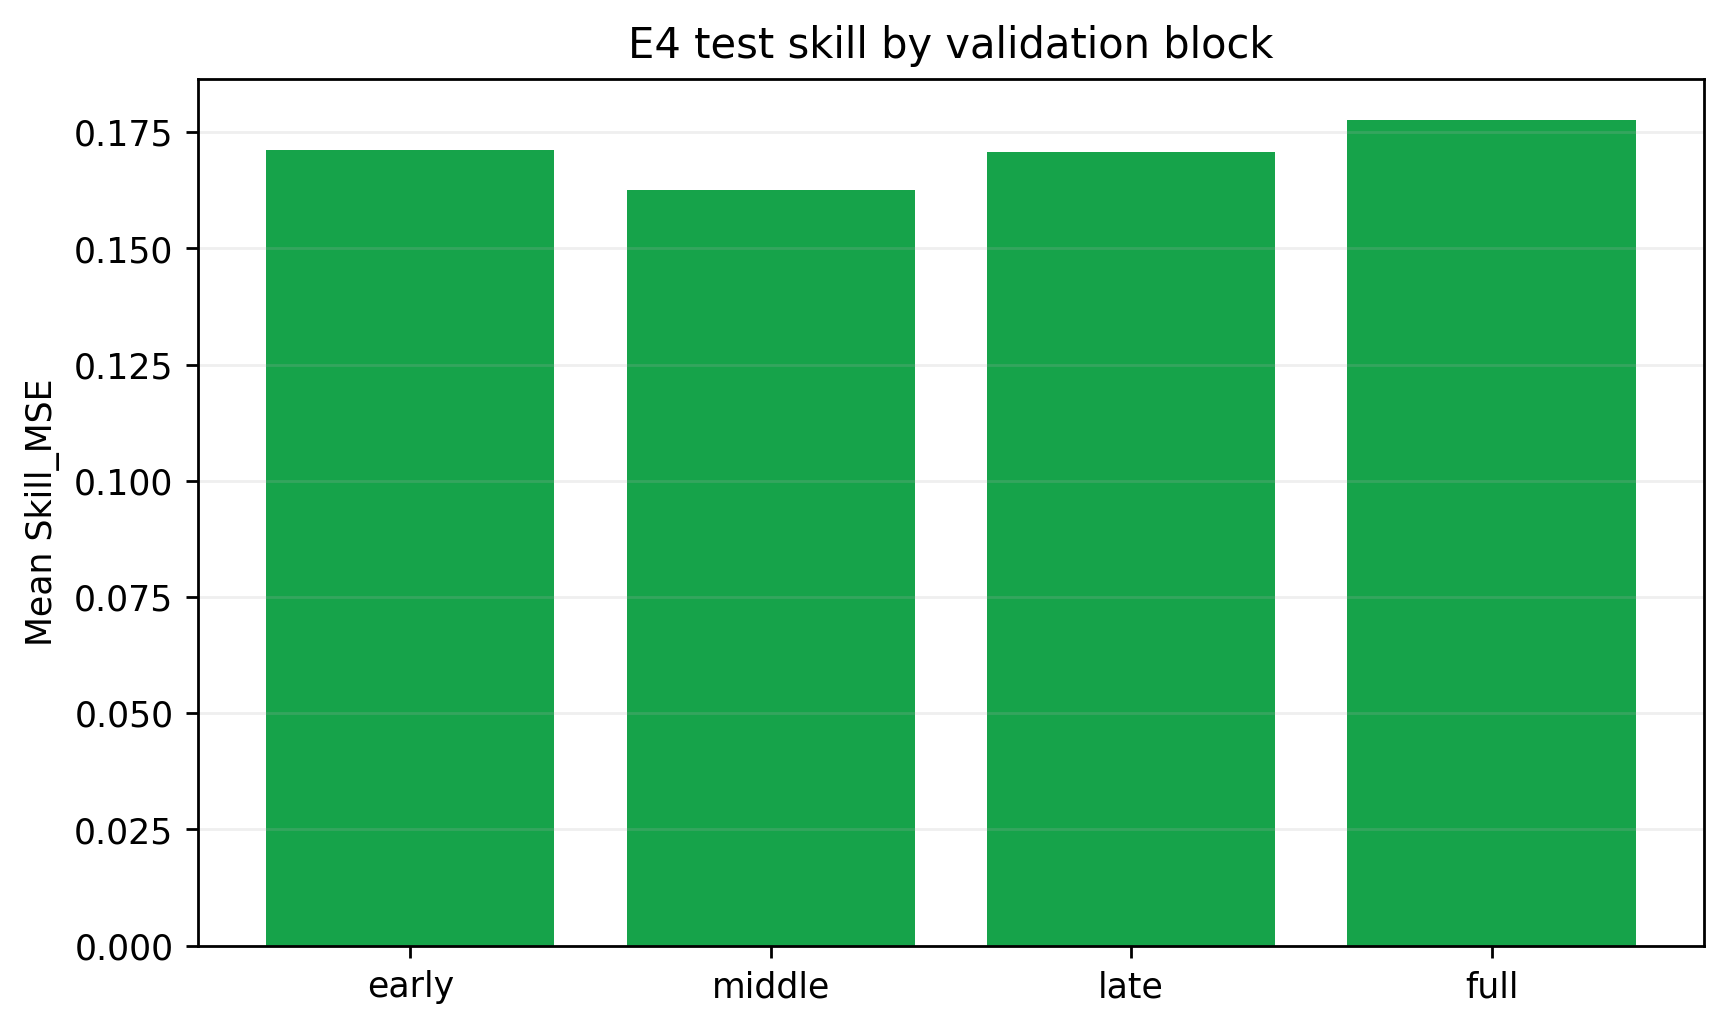
\includegraphics[width=0.95\textwidth]{paper_assets_vcea_extras/figures/E4/fig_E4_test_skill_by_block.png}
\caption{Blocked-validation test skill by calibration block. Positive transfer remains visible across blocks, but short blocks are less stable than the full validation period, supporting the frozen protocol's use of the full validation span.}
\label{fig:e4_test_skill_by_block}
\end{figure}

\begin{figure}[!t]
\centering
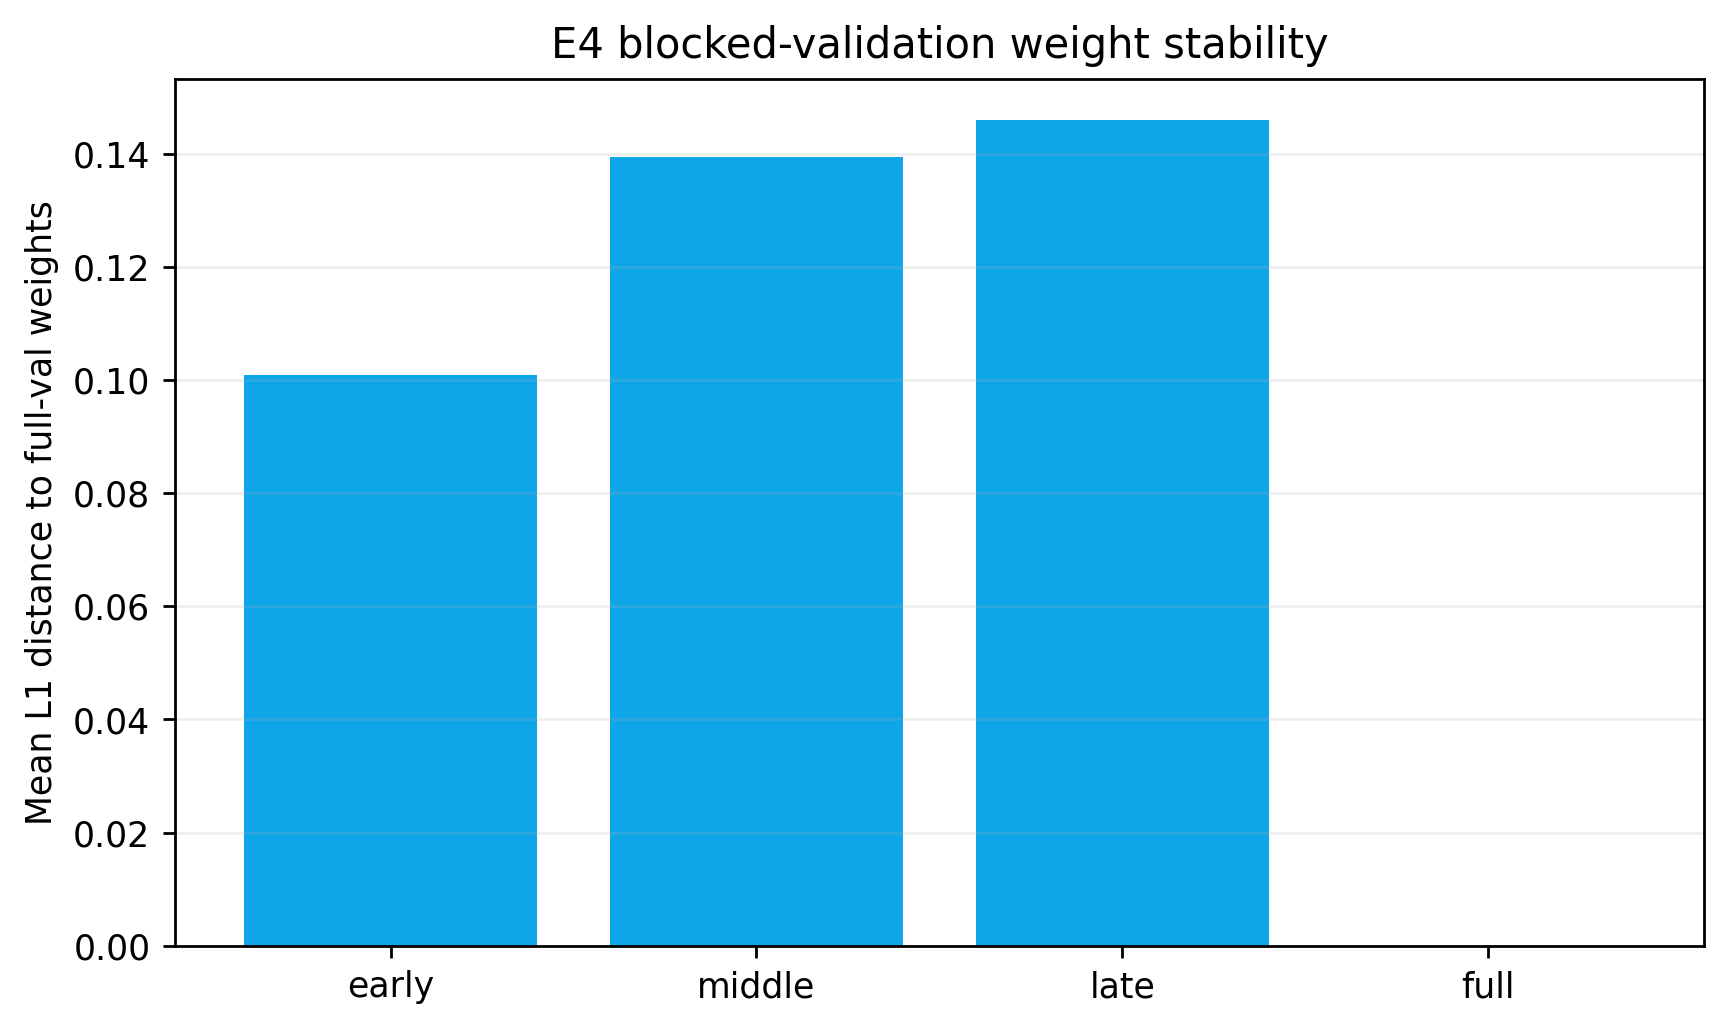
\includegraphics[width=0.95\textwidth]{paper_assets_vcea_extras/figures/E4/fig_E4_weight_stability.png}
\caption{Weight stability under blocked validation. The figure shows how far blocked-validation weights drift from the full-validation weights used in the frozen protocol.}
\label{fig:e4_weight_stability}
\end{figure}

\begin{figure}[!t]
  \centering
  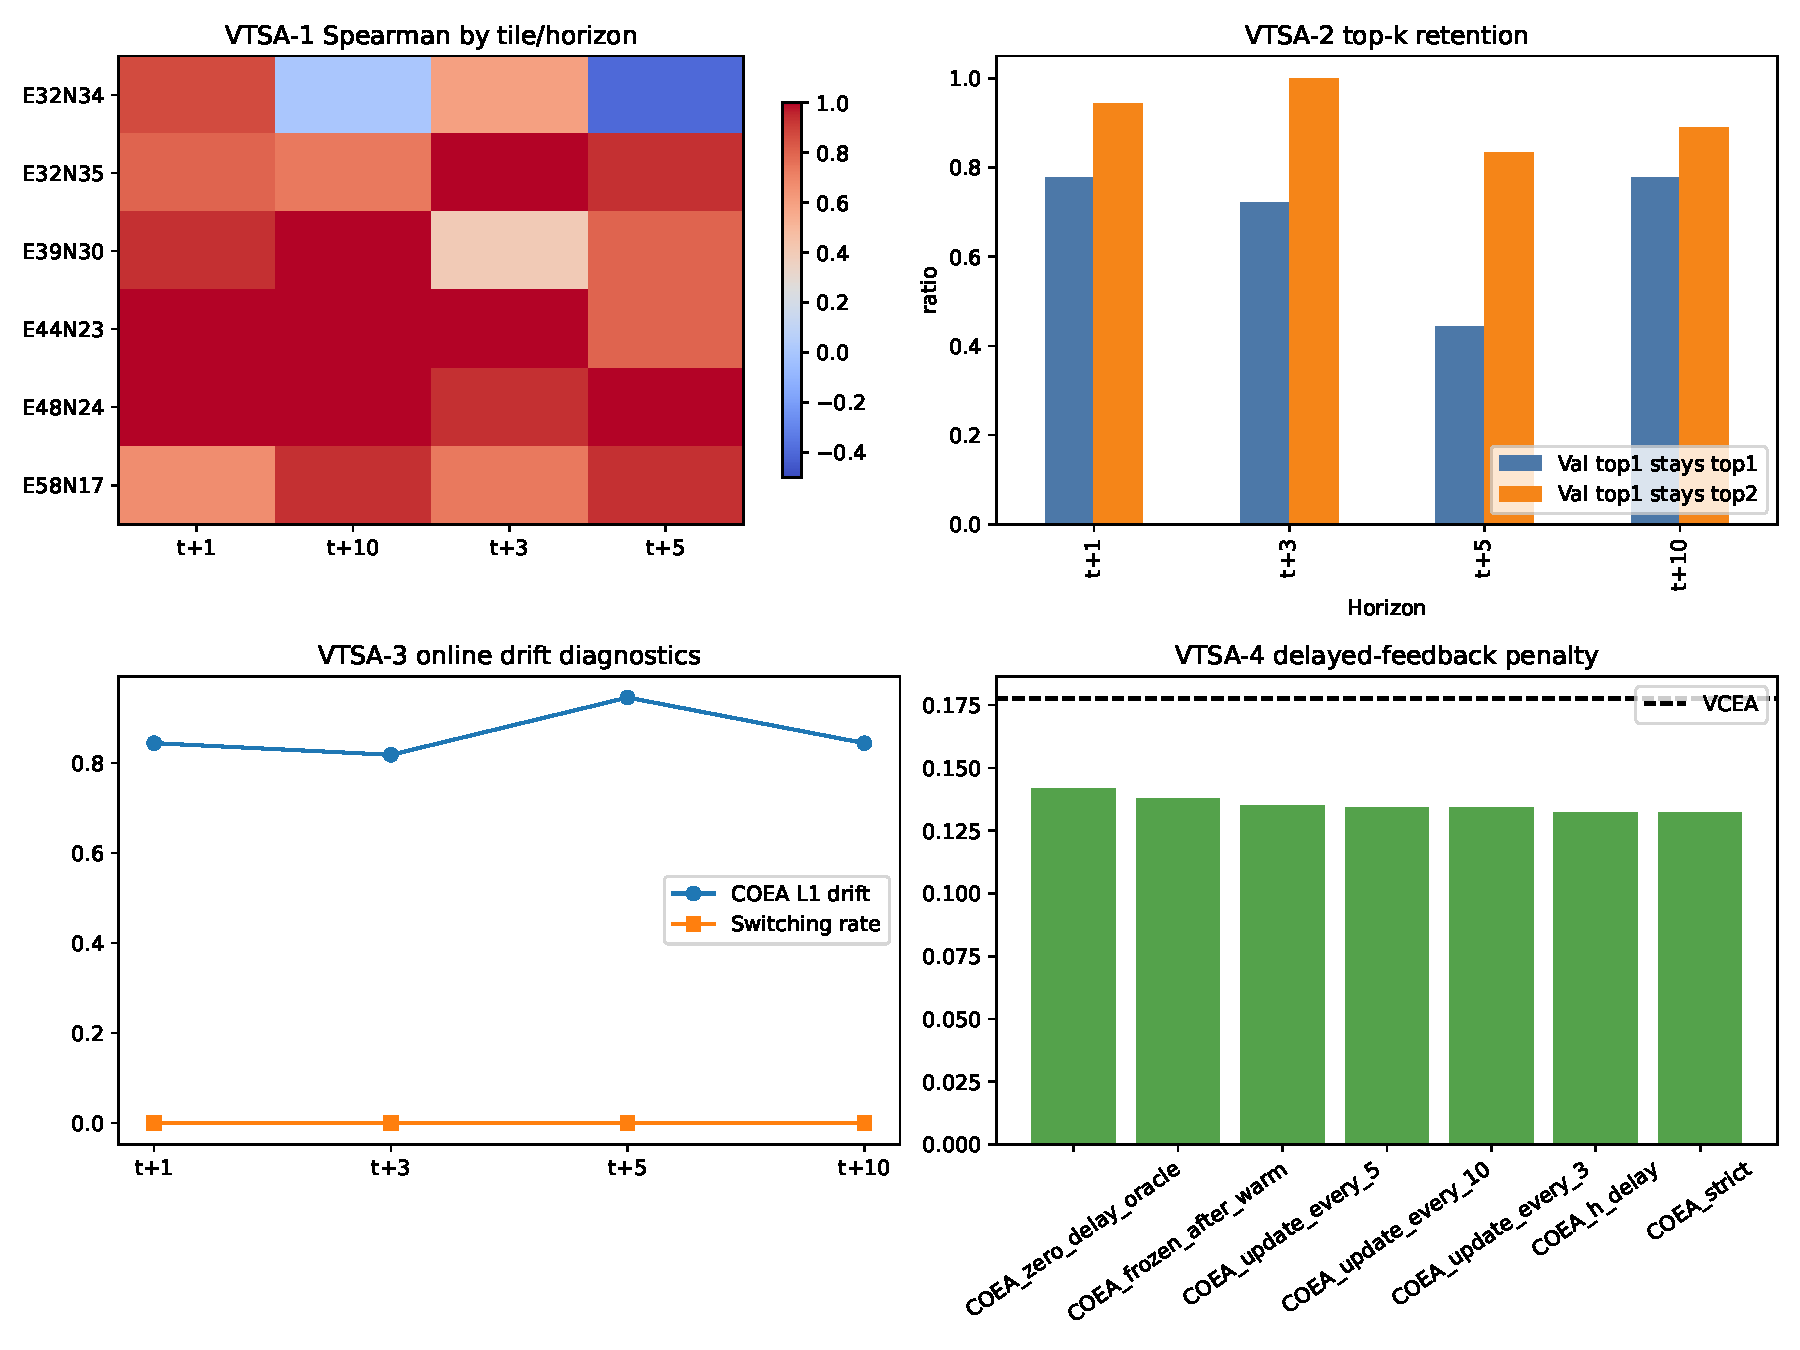
\includegraphics[width=0.95\textwidth]{figures/ready/fig_vtsa_mechanism.pdf}
  \caption{Validation-transfer stability analysis (VTSA) mechanism evidence. The figure summarizes validation-to-test rank stability, top-$k$ retention, and the drift behavior of online aggregation, providing the mechanism-level explanation for why validation-calibrated static aggregation remains competitive on the test period.}
  \label{fig:fig05}
\end{figure}

\begin{table}[!t]
  \centering
  \caption{VTSA summary metrics, including rank stability, top-$k$ retention, drift, and blocked-to-test robustness, which explain why validation-calibrated static aggregation remains effective.}
  \label{tab:table07}
  \footnotesize
  \begin{adjustbox}{max width=\textwidth}
  \begin{tabular}{p{0.22\textwidth}rp{0.54\textwidth}}
    \toprule
    VTSA metric & Value & Interpretation \\
    \midrule
    Mean Spearman & 0.778 & Validation-to-test expert ranking stability \\
    Mean Kendall & 0.731 & Rank consistency \\
    Top1 retention & 0.681 & Validation top-1 remains top-1 on test \\
    Top2 retention & 0.917 & Validation top-1 remains within test top-2 \\
    COEA mean L1 drift & 0.863 & Online weight drift relative to static weights \\
    Blocked-to-test skill & 0.173 & Static blocked-validation robustness \\
    \bottomrule
  \end{tabular}
  \end{adjustbox}
\end{table}

\begin{figure}[!t]
  \centering
  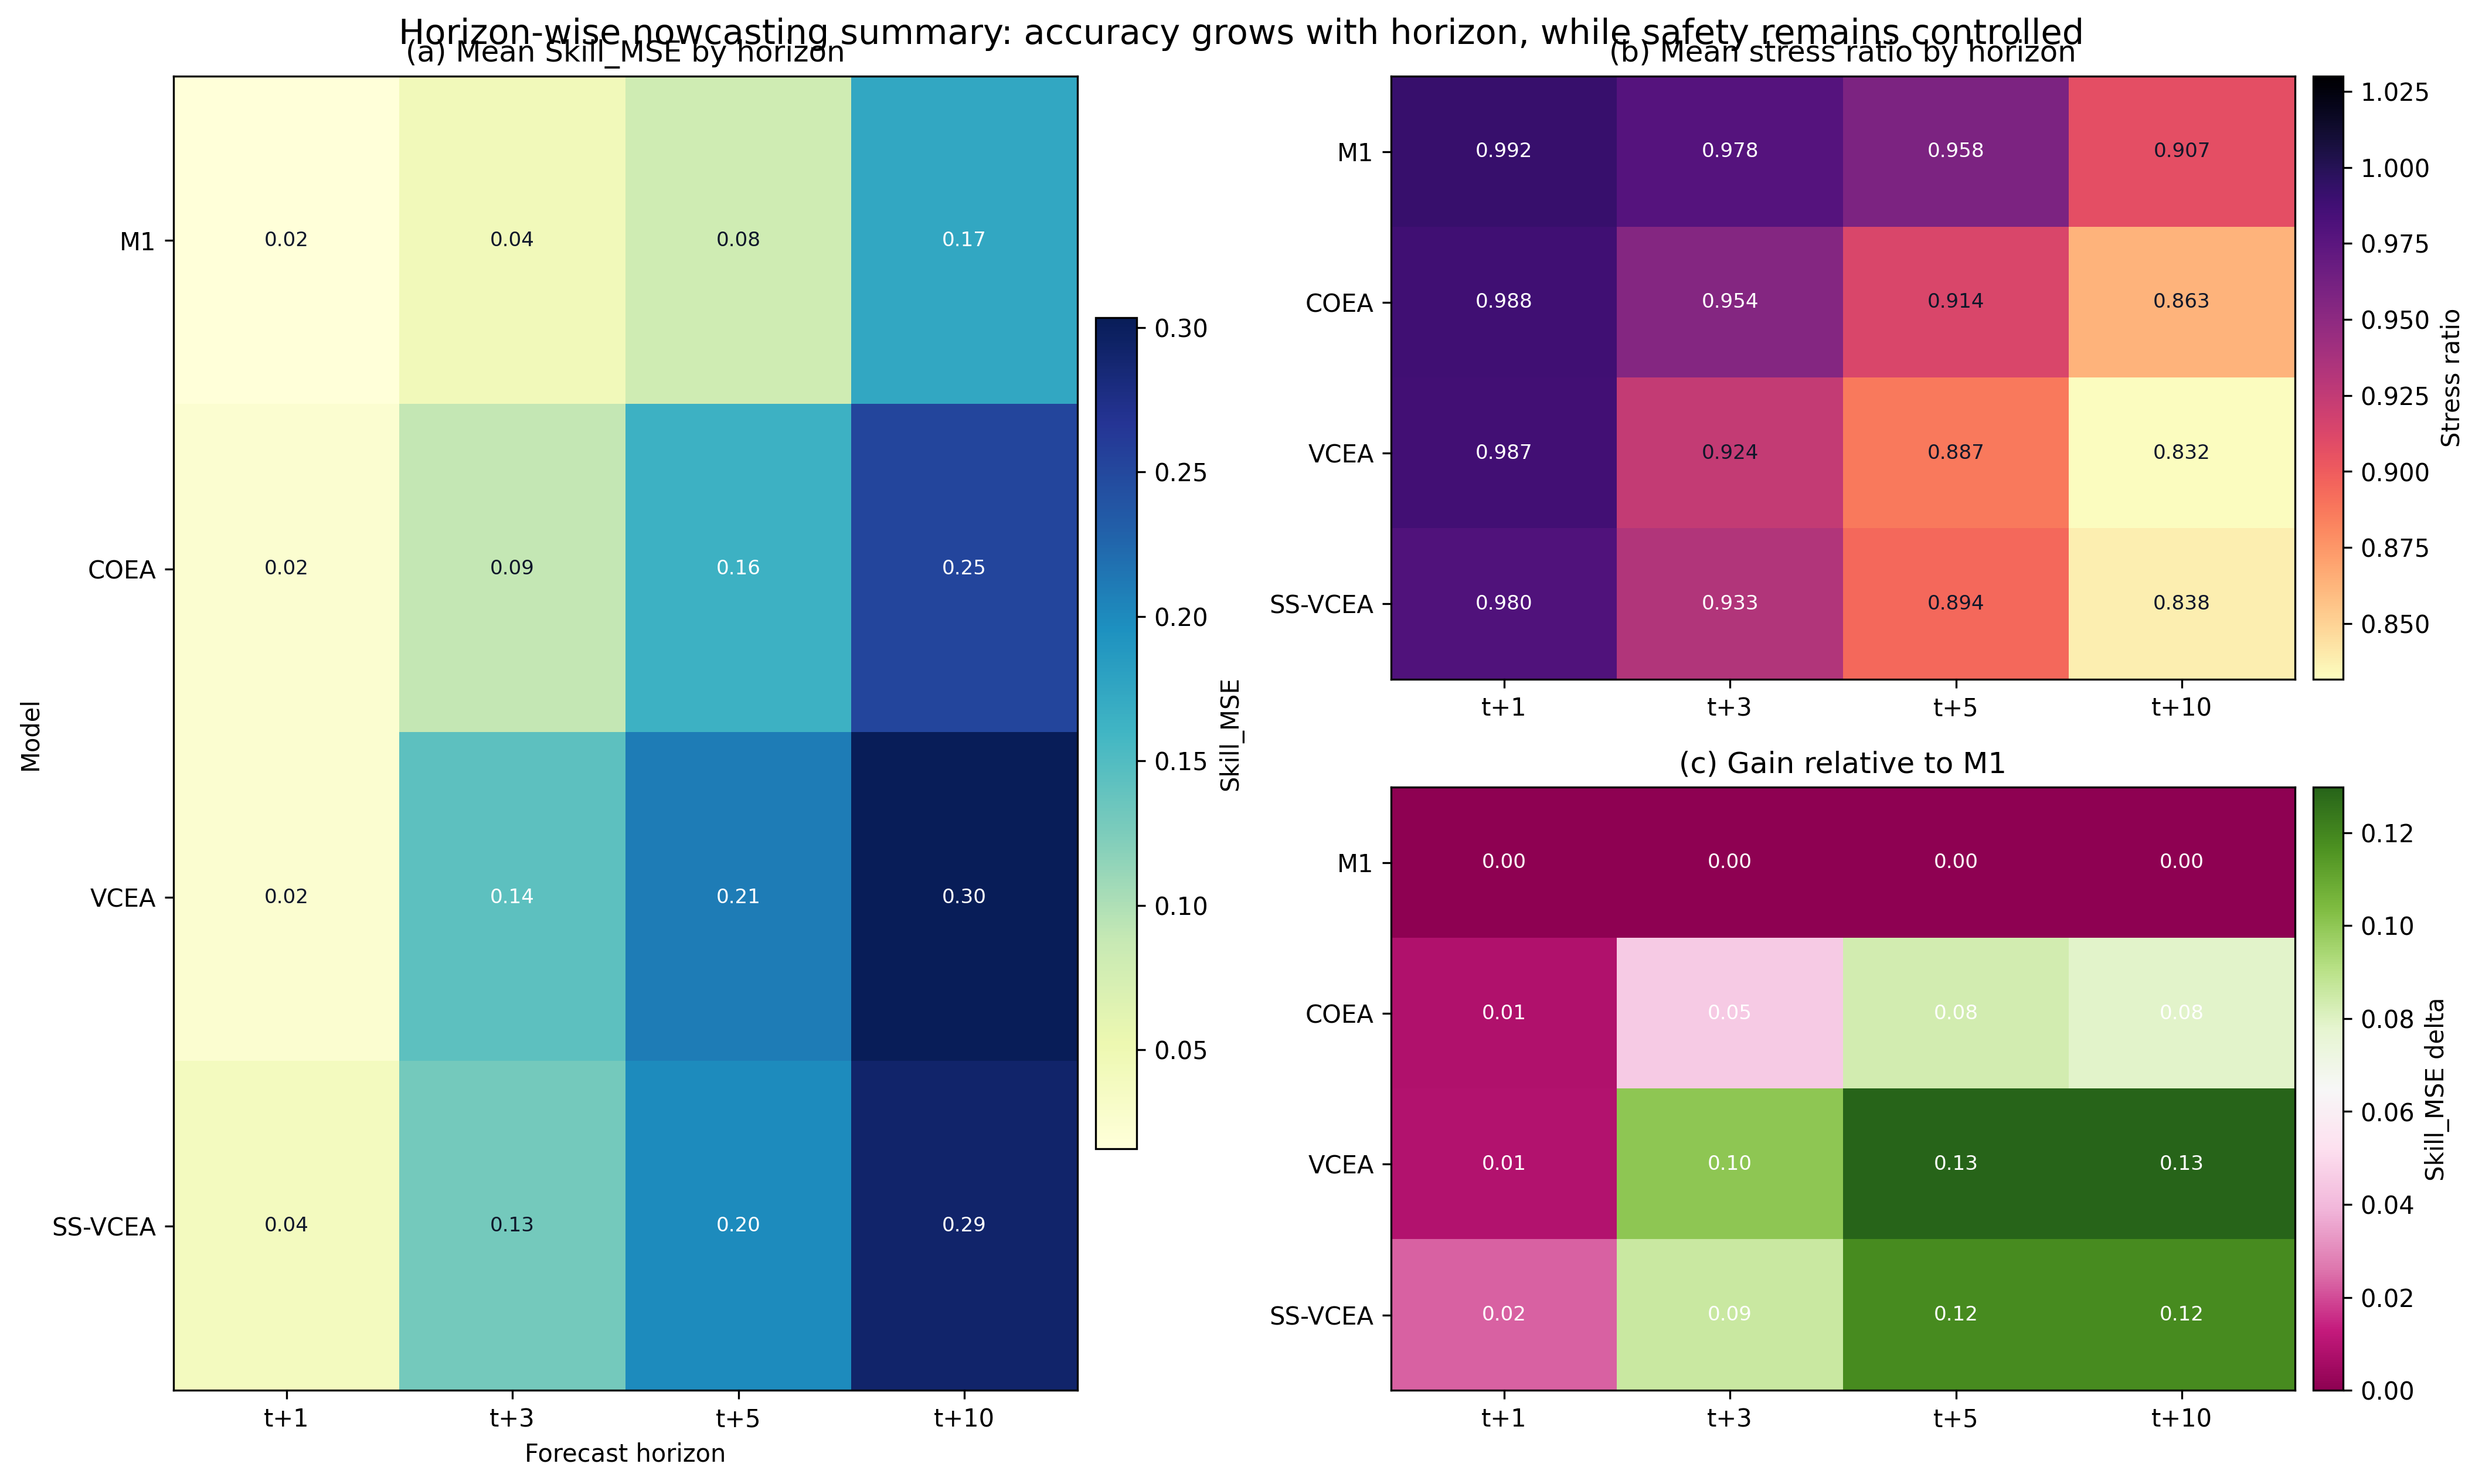
\includegraphics[width=0.95\textwidth]{figures/final/Fig07_horizon_summary_panel.png}
  \caption{Horizon-wise summary of multi-step nowcasting. (a) Mean Skill$_{\mathrm{MSE}}$ aggregated over the six main tiles. (b) Mean stress ratio by horizon. (c) Mean Skill$_{\mathrm{MSE}}$ gain relative to M1. The panel shows that aggregation gains increase with horizon, whereas stress remains controlled for COEA and SS-VCEA.}
  \label{fig:fig07}
\end{figure}

\begin{figure}[!t]
  \centering
  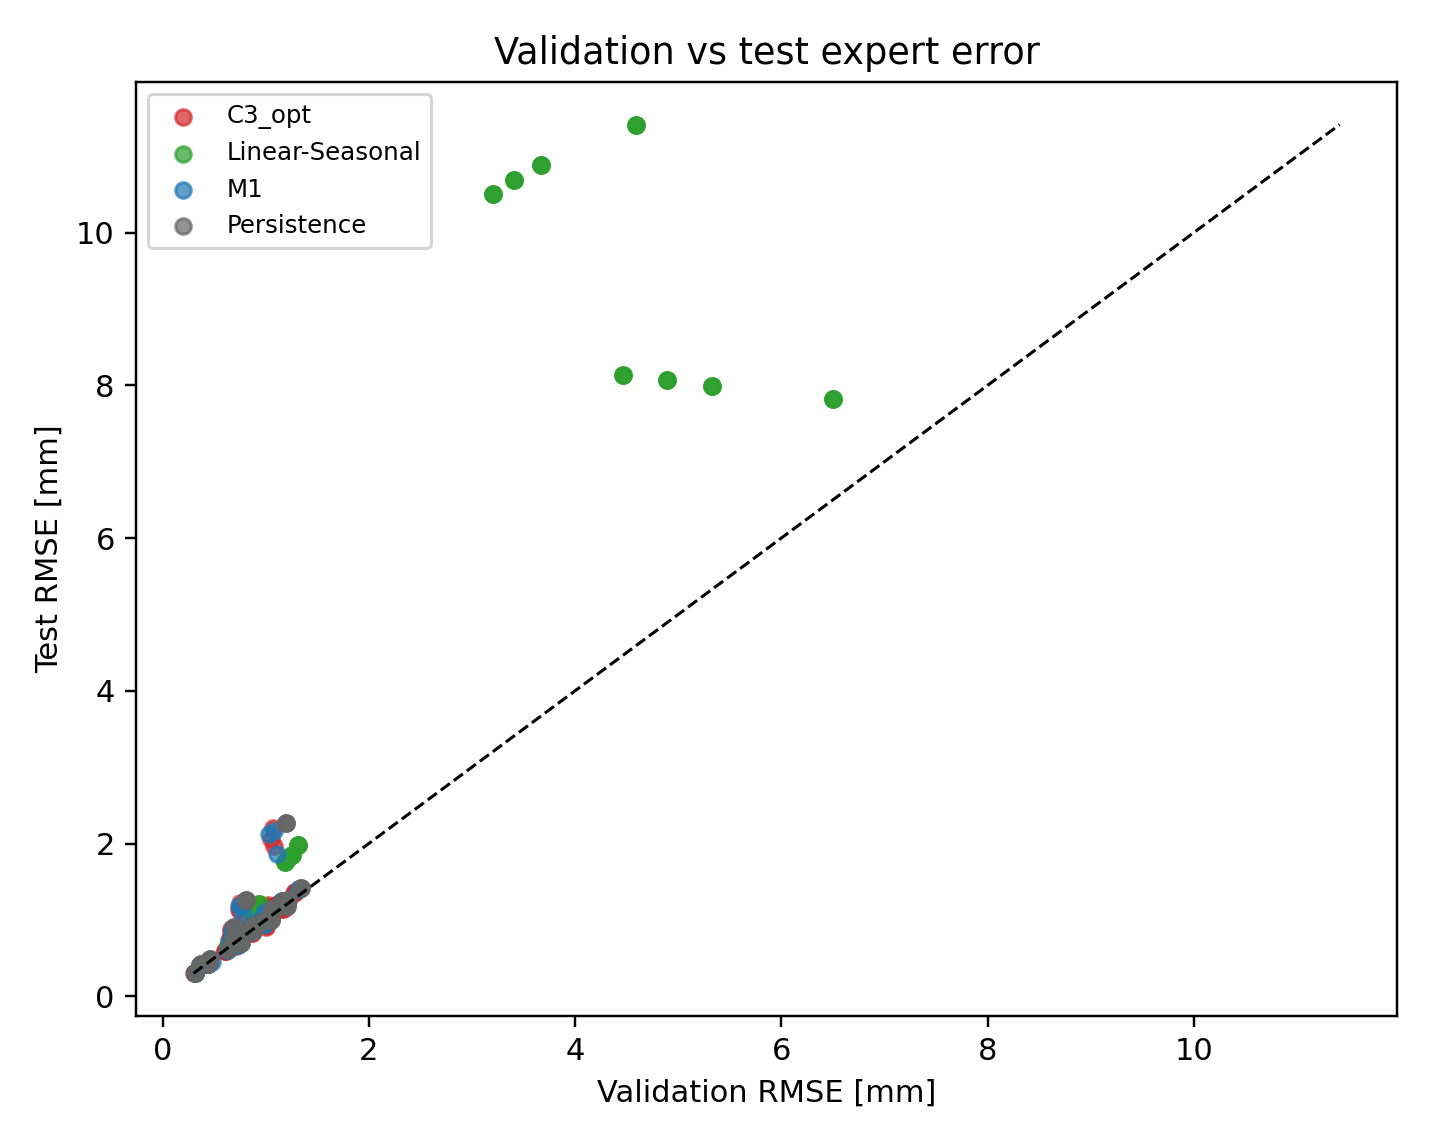
\includegraphics[width=0.95\textwidth]{figures/ready/fig_val_test_rank_scatter.png}
  \caption{Validation ranking versus test ranking for expert performance. The strong validation-to-test agreement supports the use of validation-calibrated static weights in VCEA and helps explain why static aggregation outperforms delayed-feedback online updates.}
  \label{fig:fig08}
\end{figure}

\begin{figure}[!t]
  \centering
  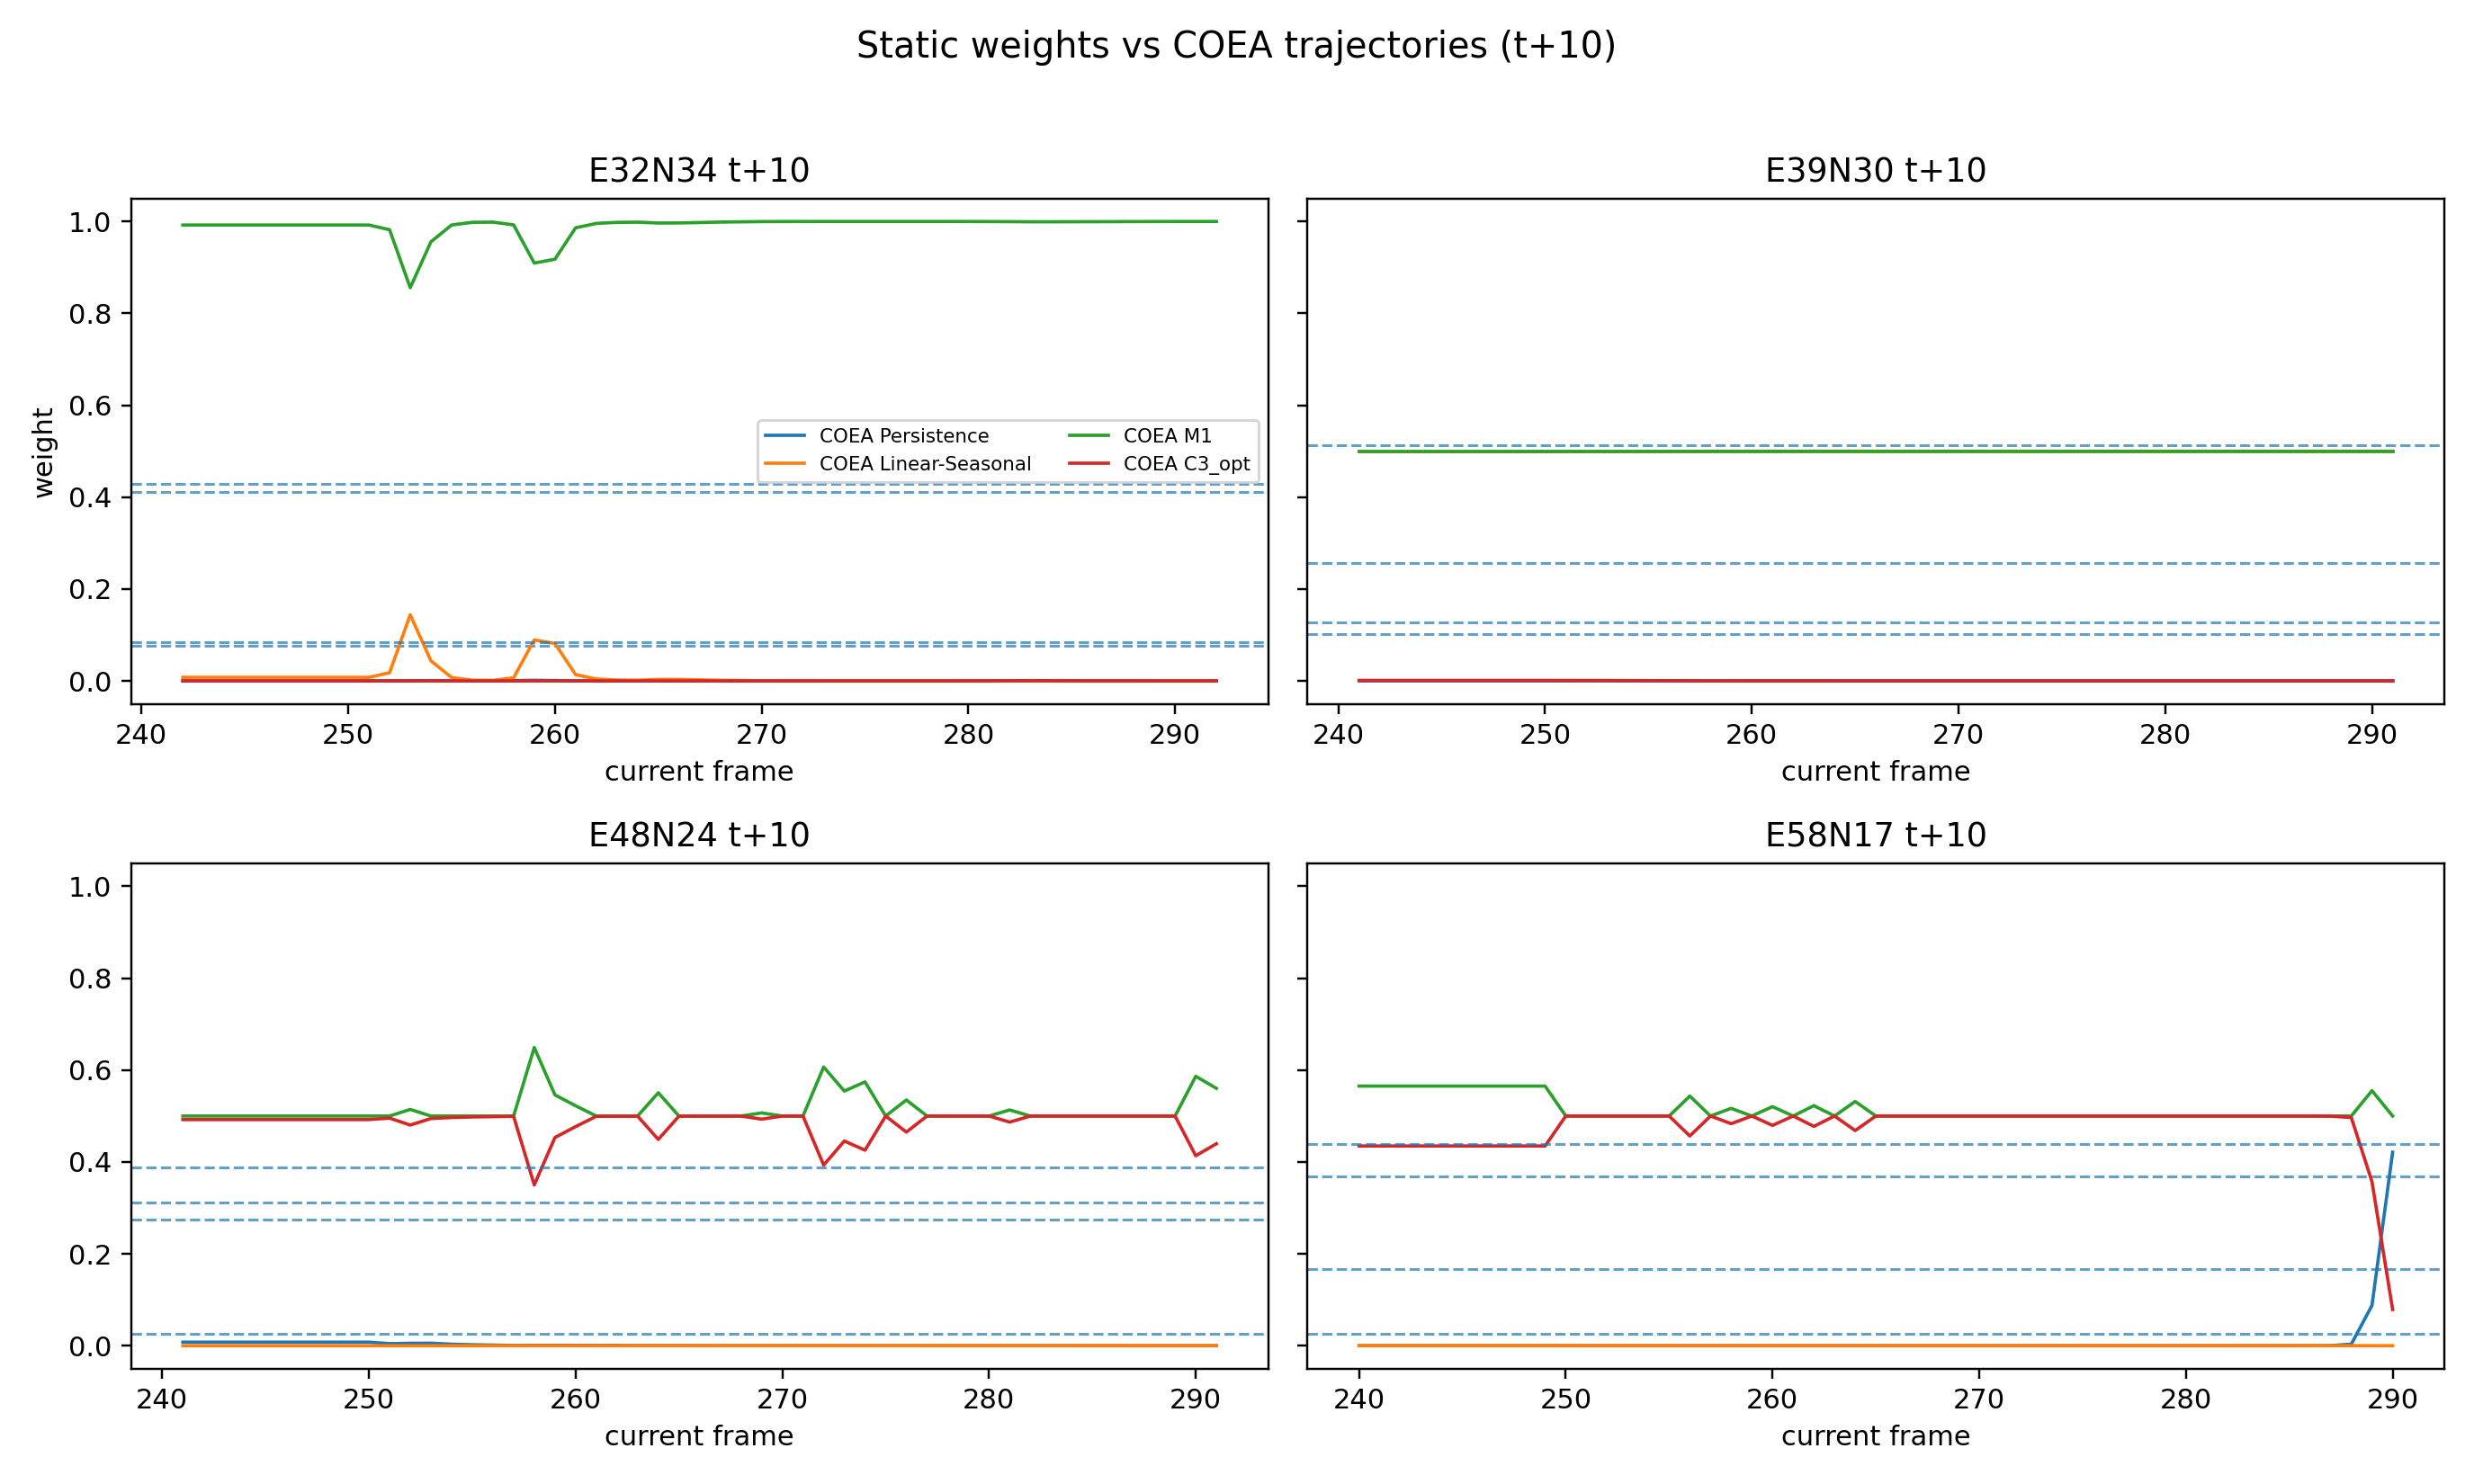
\includegraphics[width=0.95\textwidth]{figures/ready/fig_static_vs_coea_weight_drift.png}
  \caption{Weight drift from static VCEA to causal online aggregation (COEA). The drift pattern illustrates how delayed feedback and repeated online updates move the expert mixture away from the validation-calibrated optimum, which helps explain the performance gap between COEA and VCEA.}
  \label{fig:fig09}
\end{figure}

\section{Conservative Operating-Point Reference and Resolution Sensitivity}
\label{app:safety_resolution}
This appendix reports the matched conservative operating-point reference recomputation and the resolution-sensitivity package. The 0.171 VCEA value here is a matched operating-point reference rather than the primary main-six claim, and the 0.150 VCEA exact $64\times64$ value belongs to the resolution-sensitivity package only.

\begin{table}[!t]
  \centering
  \caption{Conservative operating-point trade-off between VCEA and the selected SS-VCEA q97.5 variant on the main-six and original external locked settings. The VCEA value of 0.171 is a matched operating-point reference recomputation, not the primary main-six claim.}
  \label{tab:table08}
  \footnotesize
  \begin{adjustbox}{max width=\textwidth}
  \begin{tabular}{llrrrp{0.27\textwidth}}
    \toprule
    Model & Scope & \shortstack{Mean\\Skill$_{\mathrm{MSE}}$} & \shortstack{Stress\\ratio} & \shortstack{Gain/Loss\\vs VCEA} & Note \\
    \midrule
    VCEA & main-six & 0.171 & -- & -- & matched operating-point reference, not the primary main-six claim \\
    SS-VCEA q97.5 & main-six & 0.165 & 0.992 & -0.006 & selected main-six conservative operating trade-off \\
    VCEA & external\_locked & 0.317 & 0.974 & -- & original four-tile frozen external exact evaluation \\
    SS-VCEA q97.5 & external\_locked & 0.302 & 0.974 & -0.016 & conservative operating variant \\
    \bottomrule
  \end{tabular}
  \end{adjustbox}
\end{table}

\begin{figure}[!t]
  \centering
  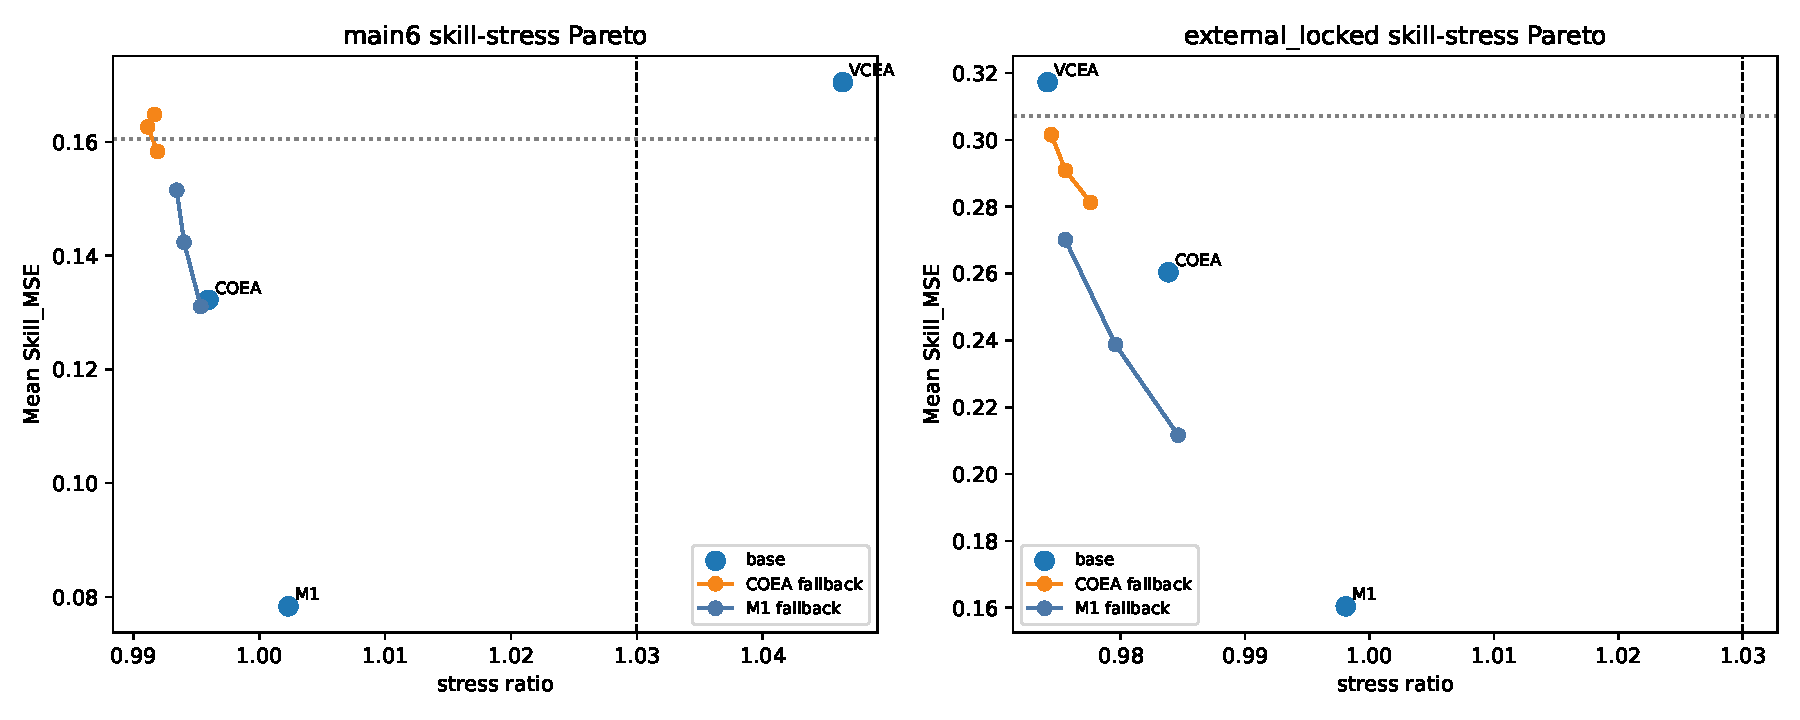
\includegraphics[width=0.95\textwidth]{figures/ready/fig_stress_skill_pareto.pdf}
  \caption{Skill--stress Pareto analysis for VCEA and SS-VCEA variants on the main-six and original external locked settings. The selected SS-VCEA q97.5 operating point sits close to the VCEA accuracy frontier while reducing the main-six stress ratio and associated over-correction pressure.}
  \label{fig:fig10}
\end{figure}

\begin{table}[!t]
  \centering
  \caption{Original four-tile frozen external summary, reporting held-out future performance under tile-local historical validation calibration without any external-based expert search or threshold retuning.}
  \label{tab:table09}
  \scriptsize
  \begin{adjustbox}{max width=\textwidth}
  \begin{tabular}{lrrrrrrr}
    \toprule
    Model & \shortstack{Skill$_{\mathrm{MSE}}$\\mean} & \shortstack{Skill$_{\mathrm{MSE}}$\\std} & \shortstack{RMSE [mm]\\mean} & \shortstack{Acc@1mm [\%]\\mean} & SSIM mean & \shortstack{Worst RMSE/\\persistence} & \shortstack{Gain/Loss\\vs VCEA} \\
    \midrule
    VCEA & 0.317 & 0.003 & 0.611 & 92.339 & 0.942 & 0.974 & 0.000 \\
    SS-VCEA q97.5 & 0.302 & 0.003 & -- & -- & -- & 0.974 & -0.016 \\
    M1 & 0.160 & 0.005 & 0.697 & 89.288 & 0.929 & 0.998 & -0.157 \\
    C3\_opt & 0.083 & 0.013 & 0.753 & 87.329 & 0.925 & 0.994 & -0.235 \\
    Persistence & 0.000 & 0.000 & 0.790 & 86.586 & 0.927 & 1.000 & -0.317 \\
    Linear-Seasonal & -0.788 & 0.000 & 0.791 & 87.434 & 0.926 & 2.966 & -1.105 \\
    \bottomrule
  \end{tabular}
  \end{adjustbox}
\end{table}

\begin{figure}[!t]
  \centering
  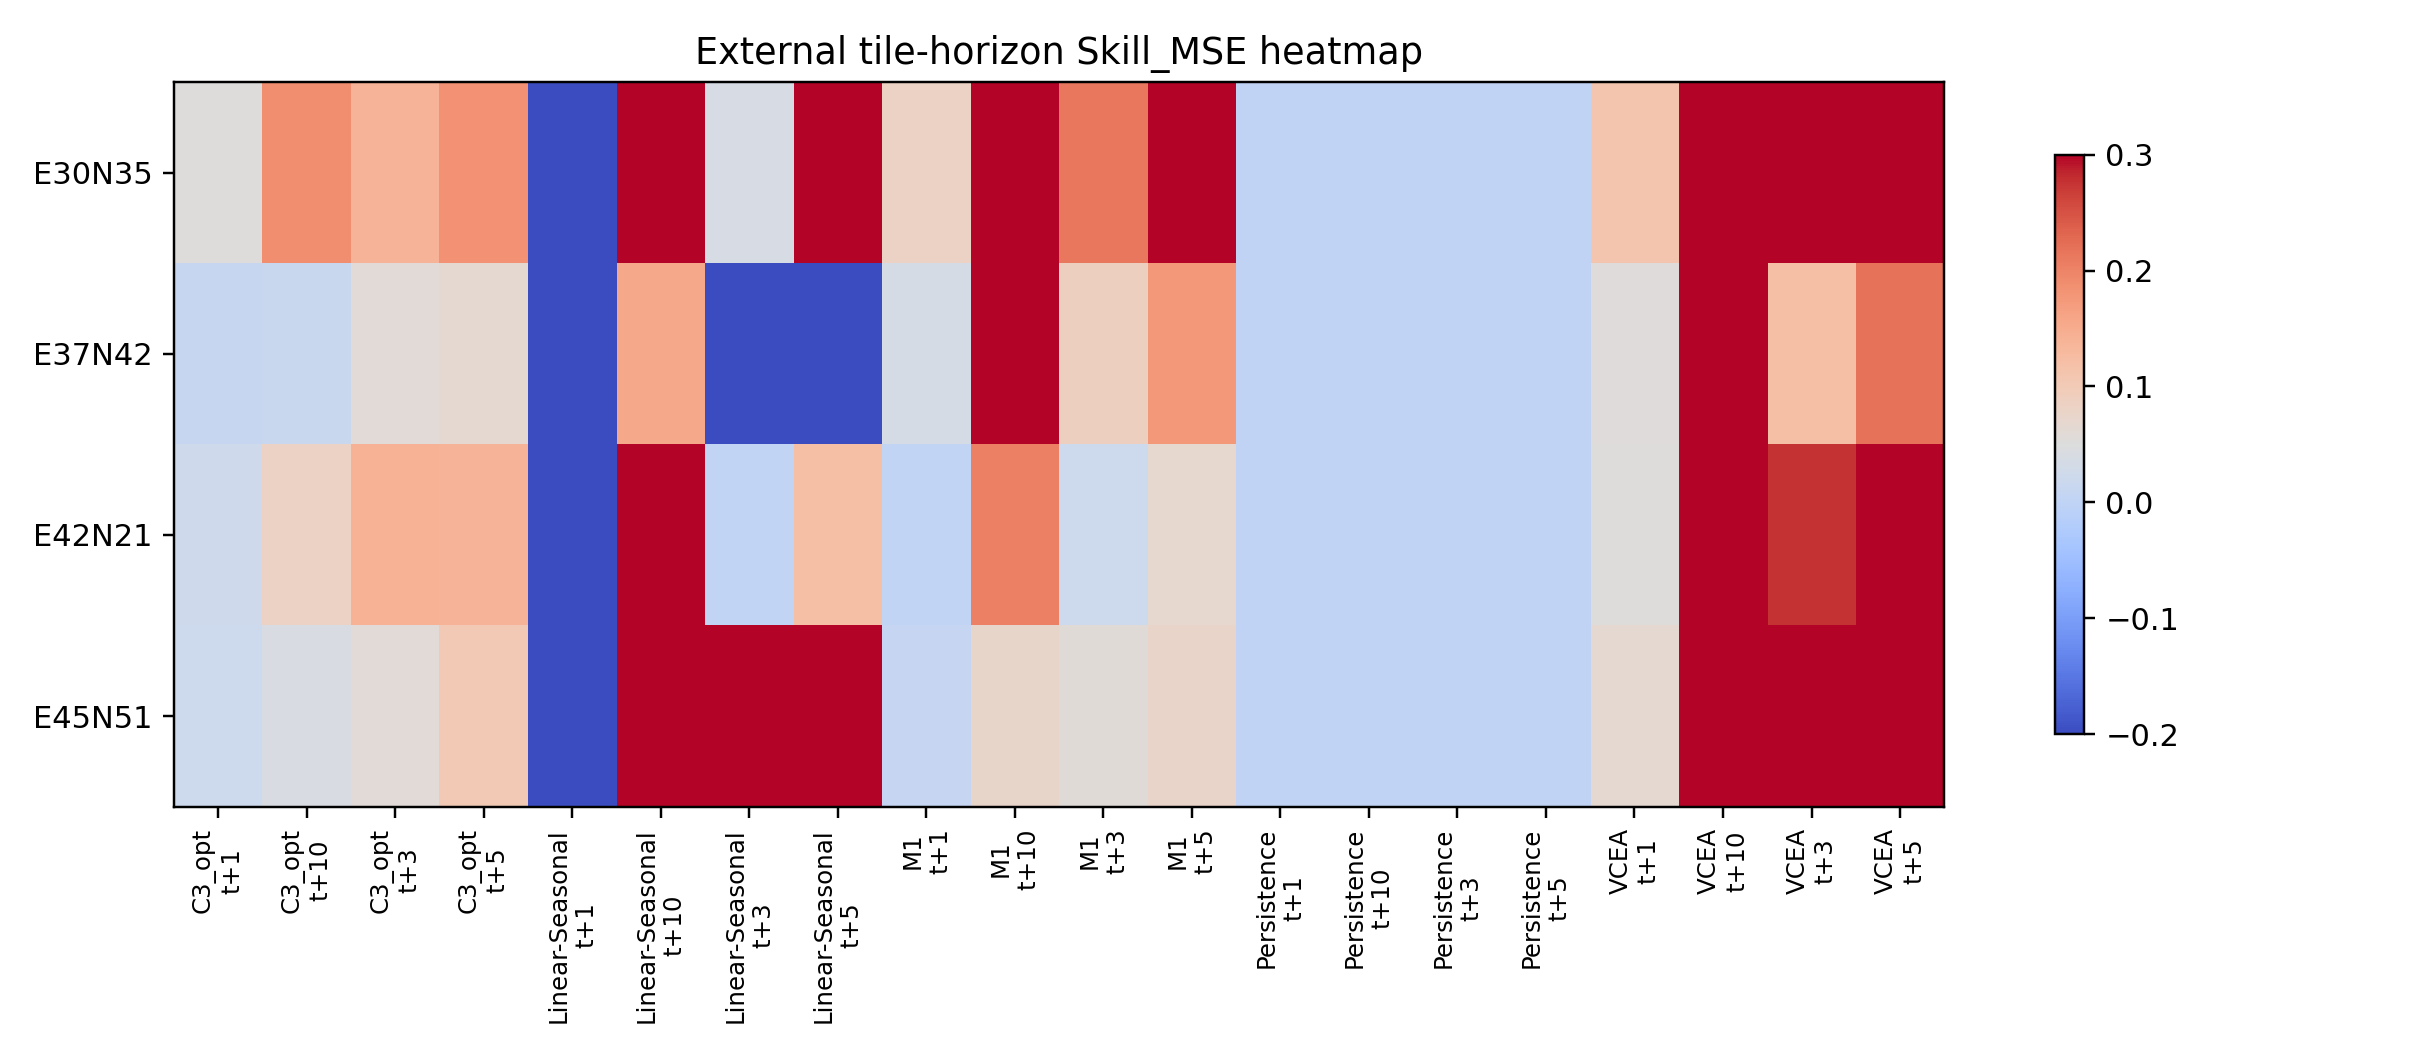
\includegraphics[width=0.95\textwidth]{figures/ready/fig_external_tile_generalization.png}
  \caption{Original four-tile frozen external results. VCEA retains positive Skill$_{\mathrm{MSE}}$ under held-out future evaluation with tile-local historical validation calibration, and SS-VCEA q97.5 offers a conservative operating alternative with limited accuracy loss.}
  \label{fig:fig11}
\end{figure}

\begin{table}[!t]
  \centering
  \caption{Resolution sensitivity across model families and aggregation types, covering the primary $64\times64$ setting and the $128\times128$ and $512\times512$ sensitivity analyses. The VCEA exact $64\times64$ value of 0.150 is sensitivity evidence only and does not replace the primary main-six claim of 0.178.}
  \label{tab:table10}
  \scriptsize
  \begin{adjustbox}{max width=\textwidth}
  \begin{tabular}{lrrrrr}
    \toprule
    Model & Resolution & \shortstack{Mean\\Skill$_{\mathrm{MSE}}$} & Mean RMSE [mm] & \shortstack{Stress\\ratio} & \shortstack{Better tiles\\vs M1} \\
    \midrule
    VCEA\_exact & 64 & 0.150 & 0.866 & 1.046 & 2 \\
    COEA\_exact & 64 & 0.129 & 0.877 & 0.997 & 3 \\
    C3\_opt & 64 & 0.084 & 0.905 & 1.011 & 2 \\
    M1 & 64 & 0.047 & 0.924 & 1.002 & 3 \\
    M0 & 64 & 0.016 & 0.936 & 1.049 & 0 \\
    Persistence & 64 & 0.000 & 0.951 & 1.000 & 0 \\
    Linear-Seasonal & 64 & -35.548 & 4.307 & 13.892 & 0 \\
    VCEA\_exact & 128 & 0.173 & 1.230 & 1.014 & 3 \\
    COEA\_exact & 128 & 0.134 & 1.261 & 0.999 & 3 \\
    C3\_opt & 128 & 0.085 & 1.295 & 1.091 & 2 \\
    M1 & 128 & 0.028 & 1.347 & 1.001 & 3 \\
    M0 & 128 & 0.016 & 1.355 & 1.012 & 0 \\
    Persistence & 128 & 0.000 & 1.371 & 1.000 & 0 \\
    Linear-Seasonal & 128 & -20.803 & 4.754 & 10.488 & 0 \\
    VCEA\_exact & 512 & 0.189 & 1.736 & 0.990 & 3 \\
    COEA\_exact & 512 & 0.145 & 1.783 & 0.999 & 3 \\
    C3\_opt & 512 & 0.116 & 1.814 & 1.054 & 3 \\
    M1 & 512 & 0.015 & 1.934 & 1.000 & 3 \\
    Persistence & 512 & 0.000 & 1.952 & 1.000 & 0 \\
    M0 & 512 & -0.010 & 1.959 & 1.032 & 0 \\
    Linear-Seasonal & 512 & -8.910 & 4.897 & 6.762 & 0 \\
    \bottomrule
  \end{tabular}
  \end{adjustbox}
\end{table}

\begin{figure}[!t]
  \centering
  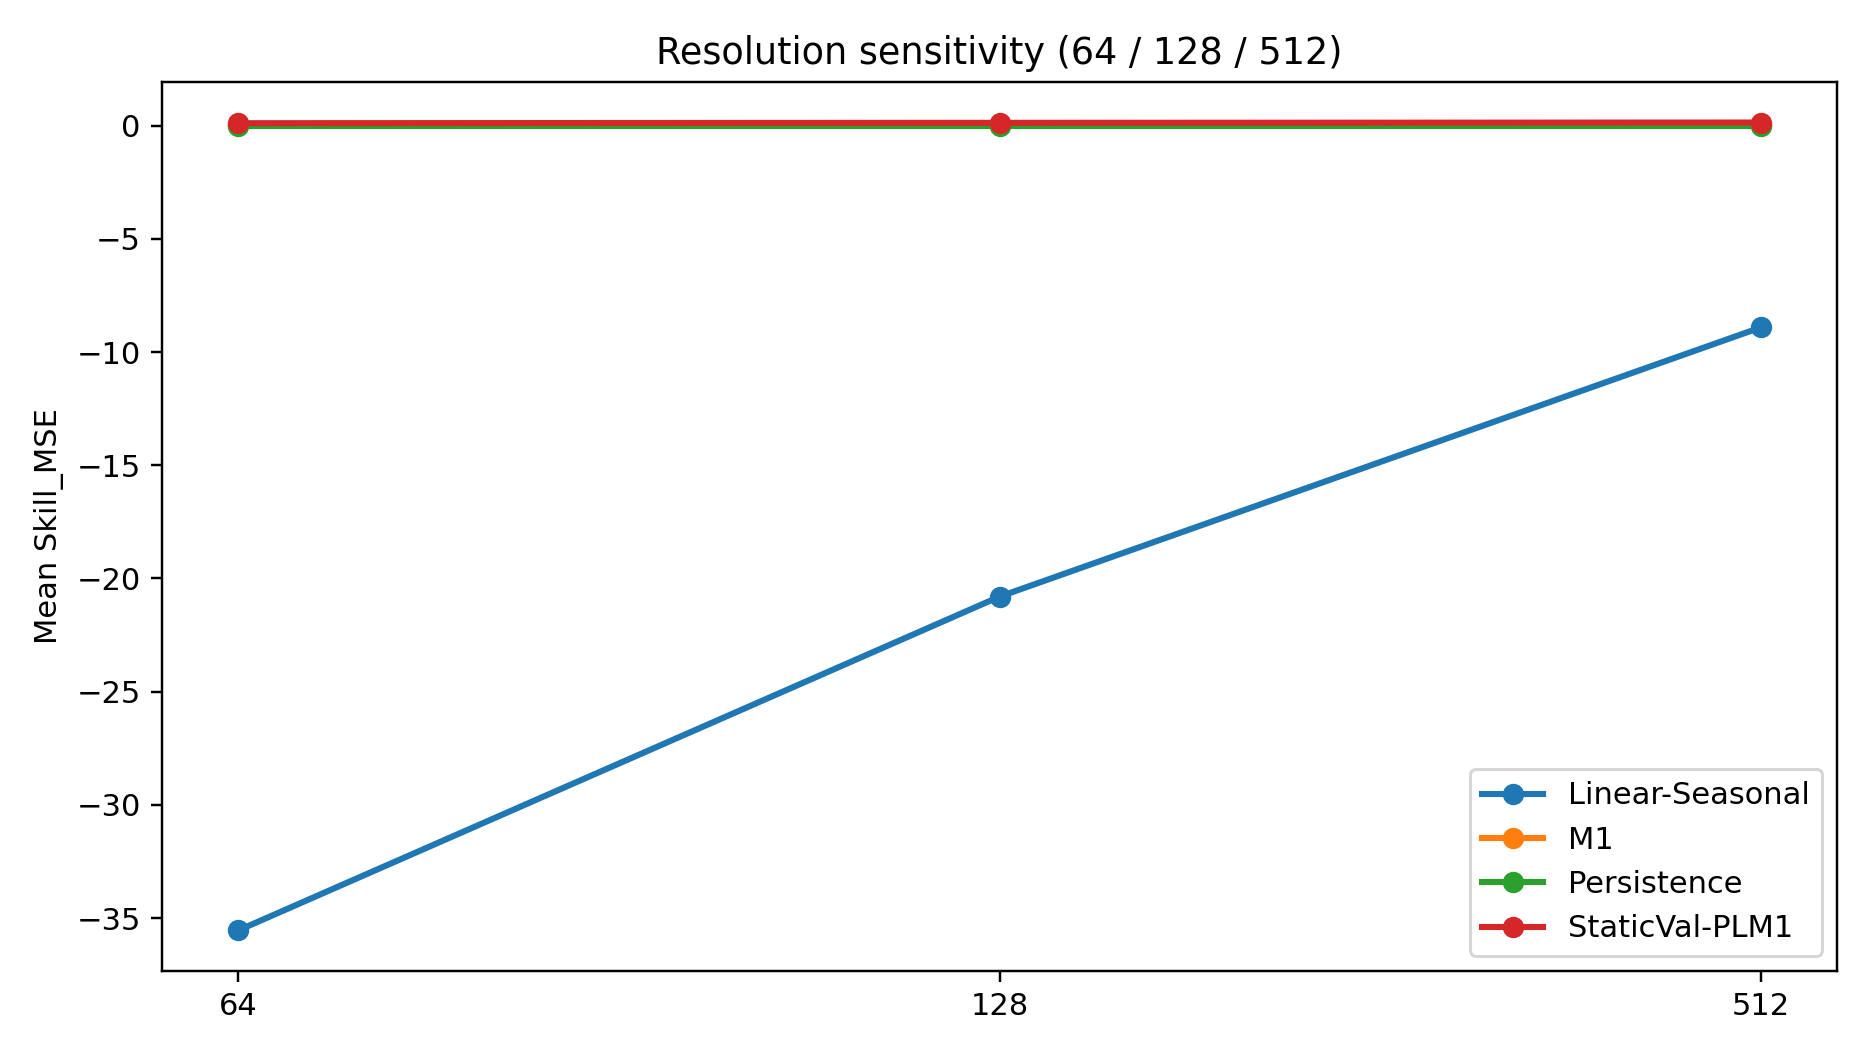
\includegraphics[width=0.95\textwidth]{figures/ready/fig_resolution_sensitivity.png}
  \caption{Resolution sensitivity of the model families. Single-model M1 degrades as the spatial grid increases from $64\times64$ to $512\times512$, whereas aggregation families continue to benefit from higher spatial resolution in sensitivity experiments. These are sensitivity results, not replacements for the primary main-six benchmark.}
  \label{fig:fig12}
\end{figure}

\section{Architecture-Search and Expert-Lineage Audit}
\label{app:architecture_audit}
This appendix summarizes the broader model-search evidence used to justify the role of neural experts within the aggregation framework.

\begin{table}[!t]
  \centering
  \caption{Architecture-search audit table summarizing the best candidate retained at each stage, its best Skill$_{\mathrm{MSE}}$, the verdict, and the reason for retention or rejection.}
  \label{tab:table11}
  \scriptsize
  \begin{adjustbox}{max width=\textwidth}
  \begin{tabular}{p{0.13\textwidth}p{0.17\textwidth}rrp{0.42\textwidth}}
    \toprule
    Stage & Best candidate & \shortstack{Best mean\\Skill$_{\mathrm{MSE}}$} & Verdict & \shortstack{Reason not final\\or role} \\
    \midrule
    V2 mainline & M1 / C2 PG-RQ-ACT & 0.078 & retained & Best robust single-model line; kept as neural expert/baseline \\
    V3 & V3-C quick & 0.013 & not retained & Too weak versus M1 despite acceptable complexity \\
    V4 & V4-C original & 0.091 & not retained & Accuracy-credible but compute-no-go \\
    V4 rescue & C3\_opt & 0.080 & not retained & Runtime fixed but full-six generalization insufficient \\
    V5 & risk-aware selector & 0.096 & not retained & Oracle space exists but learned selector under-delivers on full-six \\
    V6 & V6B\_anchor\_risk\_l20 & -0.104 & not retained & Anchored soft selector unstable and over-correction-prone \\
    V7 & COEA audited & 0.132 & retained & First successful aggregation family beyond M1 \\
    StaticVal study & VCEA & 0.178 & selected mainline configuration & Best overall accuracy trade-off in this benchmark \\
    V8 & STR-Mamba / CoMEx & 0.074 & not retained & New architectures did not beat VCEA mainline \\
    DSCF & DSCF-Full / VCEA+DSCF & 0.008 & not retained & Task-native consistency direction did not pass the quick gate \\
    \bottomrule
  \end{tabular}
  \end{adjustbox}
\end{table}

\begin{figure}[!t]
  \centering
  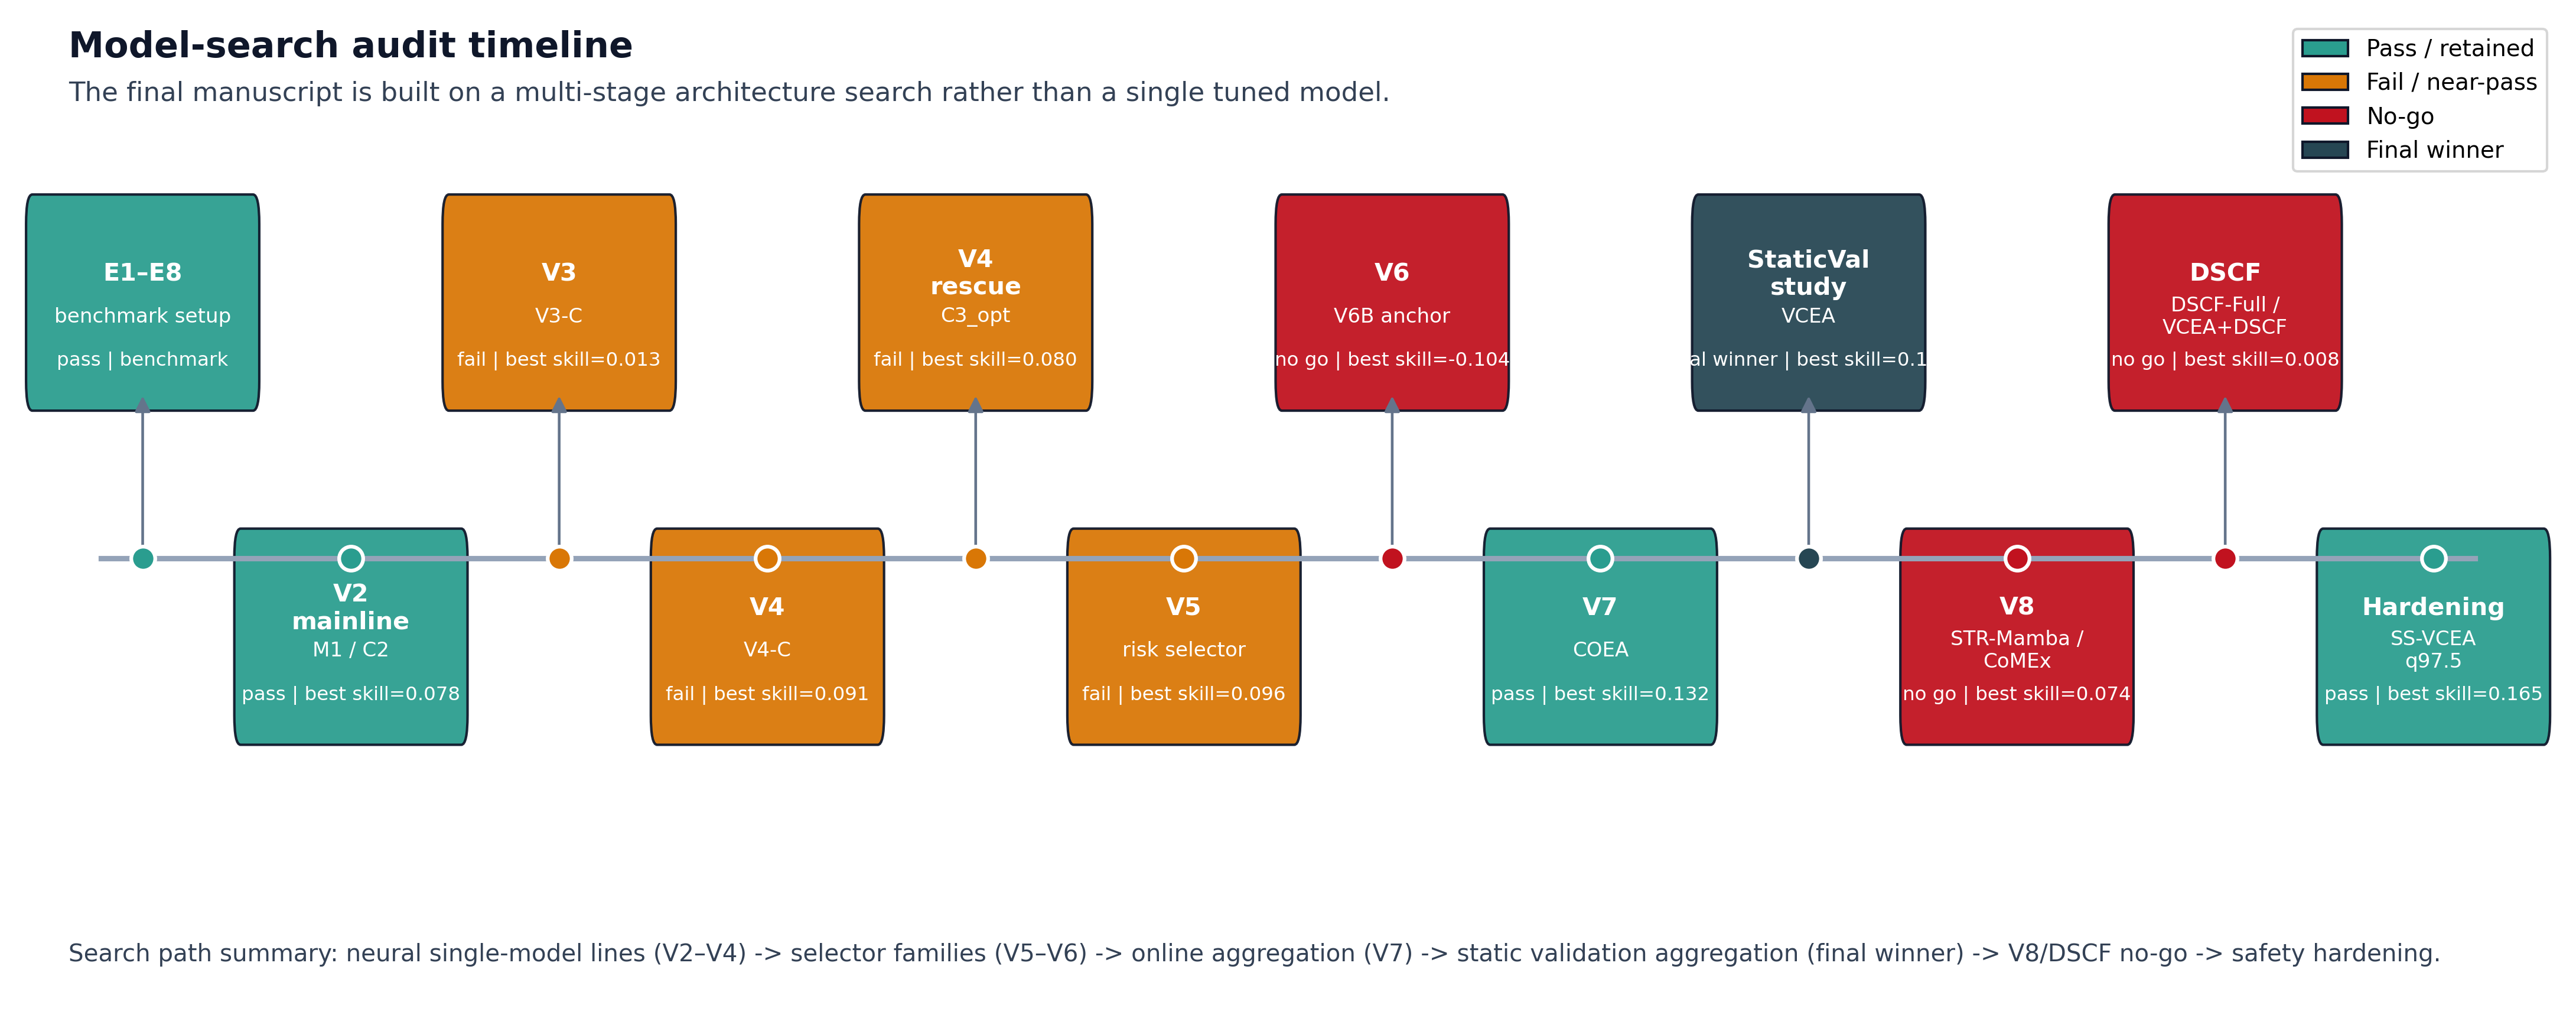
\includegraphics[width=0.95\textwidth]{figures/final/Fig13_model_search_audit_timeline.png}
  \caption{Model-search audit timeline across the preliminary model-search experiments. The final manuscript is supported by a staged architecture search rather than a single tuned model: robust single-model baselines, selector families, online aggregation, static validation aggregation, and conservative operating-point reference studies were all evaluated before freezing the mainline.}
  \label{fig:fig13}
\end{figure}

\begin{figure}[!t]
  \centering
  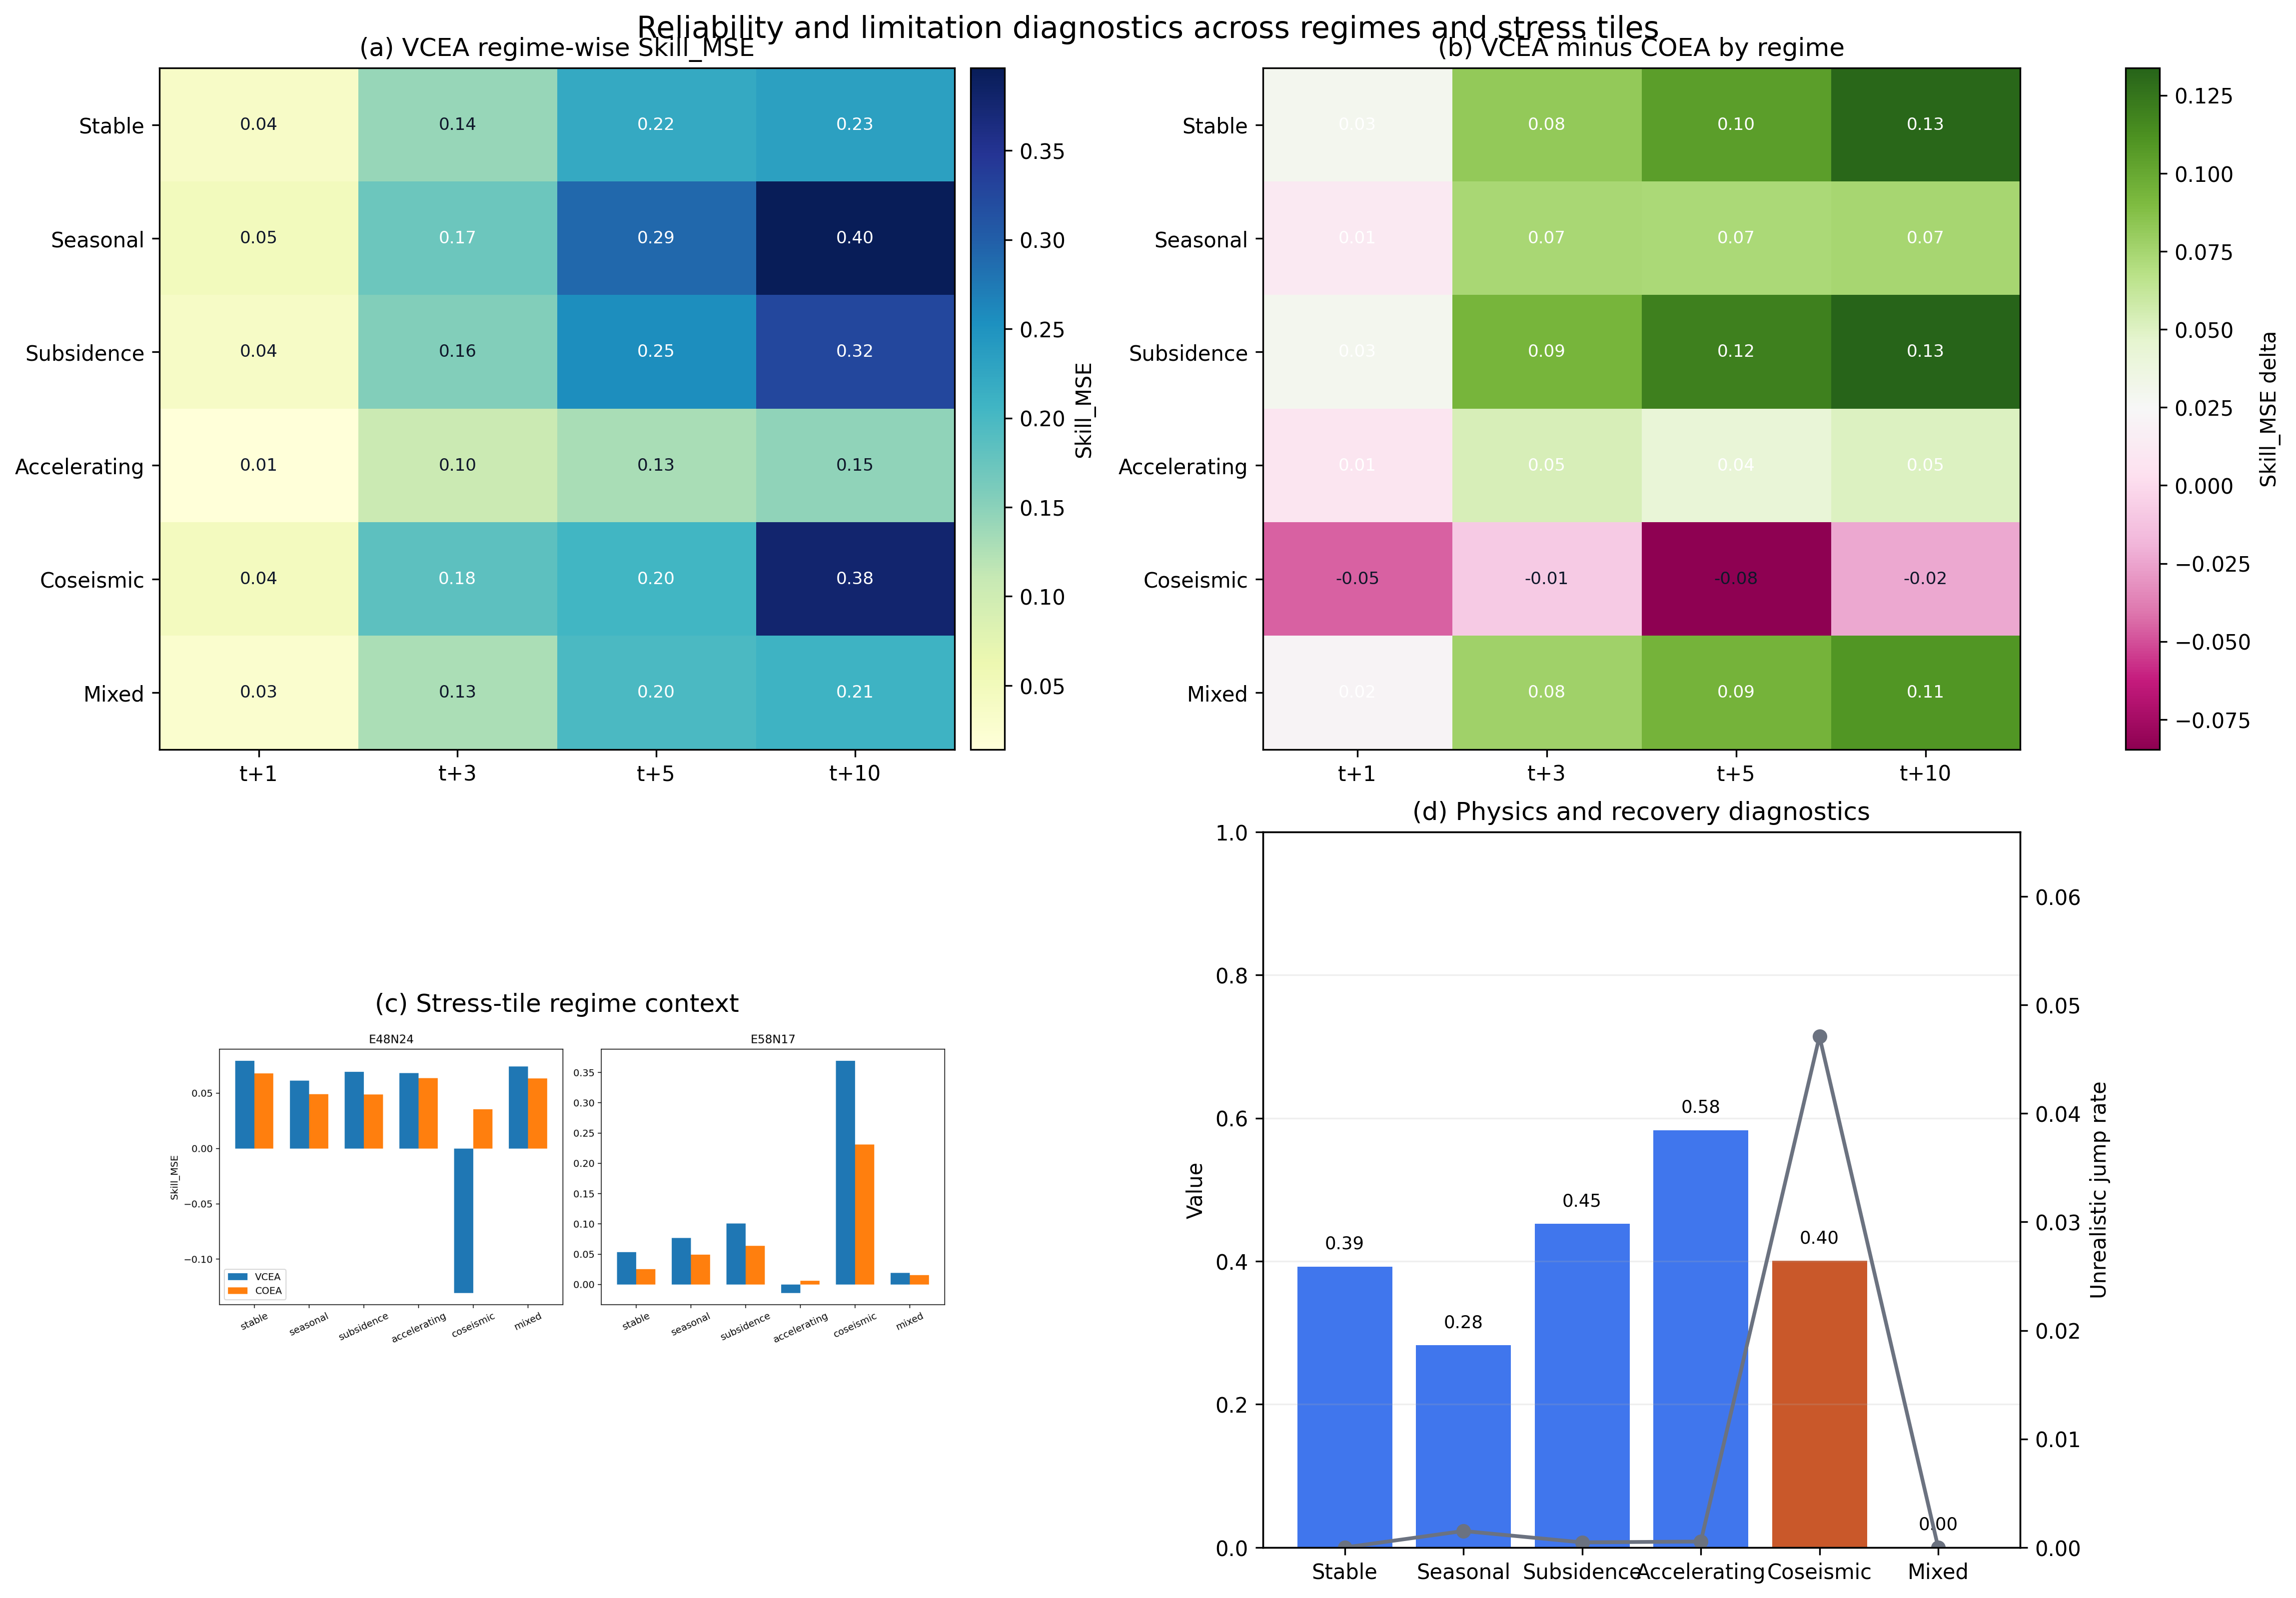
\includegraphics[width=0.95\textwidth]{figures/final/Fig14_physics_regime_diagnostic_panel.png}
  \caption{Reliability and limitation diagnostics across regimes and stress tiles. (a) Regime-wise Skill$_{\mathrm{MSE}}$ of VCEA by horizon. (b) Regime-wise difference between VCEA and COEA. (c) Stress-tile regime context. (d) Physics-oriented diagnostics including sign consistency, post-event recovery ratio, and unrealistic jump behavior. These panels show that gains are not uniform across regimes and that coseismic cases remain the hardest operating condition.}
  \label{fig:fig14}
\end{figure}

\section{Reproducibility and Asset Traceability}
\label{app:repro_trace}
This appendix keeps the compact traceability tables that map manuscript claims to frozen data products, split definitions, cache provenance, and audit assets.

\begin{table}[!t]
  \centering
  \caption{Reproducibility package and provenance map, listing the manifests, split definitions, cache registries, and claim-to-result tracing artifacts that support the manuscript.}
  \label{tab:table12}
  \scriptsize
  \begin{adjustbox}{max width=\textwidth}
  \begin{tabular}{p{0.18\textwidth}p{0.46\textwidth}p{0.25\textwidth}}
    \toprule
    Artifact & Path & Role \\
    \midrule
    Product manifest & \path{data/manifests/product_manifest.csv} & Data product provenance \\
    Tile manifest & \path{data/manifests/tile_manifest.csv} & Main/external tile provenance \\
    Resolution manifest & \path{data/manifests/resolution_manifest.csv} & 64/128/512 scope freeze \\
    Main split & \path{splits/main6_train_val_test.json} & Formal primary main-six split \\
    External locked split & \path{splits/external4_locked_eval.json} & Frozen original external evaluation \\
    Expert cache registry & \path{cache/expert_cache_registry.yaml} & Expert prediction cache provenance \\
    Aggregation weight registry & \path{cache/aggregation_weight_registry.yaml} & Aggregation calibration provenance \\
    Lineage table & \path{reproducibility/result_lineage_table.csv} & Experiment-to-artifact mapping \\
    Claim-to-result map & \path{reproducibility/claim_to_result_map.md} & Claim audit \\
    Paper table source map & \path{reproducibility/paper_table_source_map.csv} & Table-to-source provenance \\
    Figure source map & \path{reproducibility/figure_source_map.csv} & Figure-to-source provenance \\
    Exact/proxy/transfer flags & \path{reproducibility/exact_proxy_transfer_flags.csv} & Historical artifact status \\
    \bottomrule
  \end{tabular}
  \end{adjustbox}
\end{table}

The table uses paper-facing reproducibility-package paths rather than internal archive directory names.

\begin{table}[!t]
\centering
\footnotesize
\begin{adjustbox}{max width=\textwidth}
\begin{tabular}{p{0.23\textwidth}p{0.58\textwidth}}
\toprule
Item & Value \\
\midrule
Python version & 3.13.5 \\
PyTorch version & 2.11.0+cu128 \\
CUDA stack & cu128 build; CUDA available = True \\
GPU / CPU & NVIDIA GeForce RTX 3090 Ti; 12th Gen Intel(R) Core(TM) i5-12600K \\
OS & Windows-11-10.0.26200-SP0 \\
Main random seeds & 42, 43, 44 \\
Main scripts / configs & \path{run_vcea_extra_experiments.py}, \path{run_vcea_e7_pan_europe_audit_strong.py}, \path{splits/main6_train_val_test.json}, \path{outputs/tgrs_2019_2023/vcea_extra_experiments/E7_pan_europe_locked_audit_strong/configs/config_E7_frozen_audit.yaml} \\
\bottomrule
\end{tabular}
\end{adjustbox}
\caption{Compact software, hardware, and seed summary for the reproducibility package. Values are drawn from the frozen environment manifest, the extra-experiment environment file, and the archived seed registry.}
\label{tab:repro_environment}
\end{table}

\begin{table}[!t]
\centering
\scriptsize
\begin{adjustbox}{max width=\textwidth}
\begin{tabular}{p{0.20\textwidth}p{0.17\textwidth}p{0.20\textwidth}p{0.20\textwidth}p{0.13\textwidth}}
\toprule
Manuscript claim & Evidence table / figure & Source CSV / JSON & Protocol caveat & Manuscript location \\
\midrule
VCEA improves over M1 on the primary main-six benchmark & Table~\ref{tab:table06}, Appendix Fig.~\ref{fig:fig06} & \path{outputs/tgrs_2019_2023/staticval_ea_study/final_aggregation_comparison.csv} & exact 64$\times$64 main-six benchmark & Secs.~III--VI-A \\
Split-boundary leakage does not explain the gain & Table~\ref{tab:e1_leakage_audit}, Fig.~\ref{fig:e1_skill_delta_by_tile} & \path{paper_assets_vcea_extras/tables_csv_original/E1_E6/table_E1_leakage_audit.csv} & stricter protocols recalibrate aggregation without retraining experts & Sec.~VI-B \\
Heterogeneous experts matter & Table~\ref{tab:e2_expert_ablation_main6}, Fig.~\ref{fig:e2_expert_weights} & \path{paper_assets_vcea_extras/tables_csv_original/E1_E6/table_E2_expert_ablation_main6.csv} & expert pool fixed before external audits & Sec.~VI-C \\
Tile+horizon validation calibration matters & Table~\ref{tab:e3_calibration_ablation}, Fig.~\ref{fig:e3_calibration_barplot} & \path{paper_assets_vcea_extras/tables_csv_original/E1_E6/table_E3_calibration_ablation.csv} & oracle row is diagnostic only, not an operational setting & Sec.~VI-D \\
SS-VCEA q97.5 provides a conservative skill--stress trade-off & Table~\ref{tab:e6_threshold_sweep}, Fig.~\ref{fig:e6_skill_stress_frontier} & \path{paper_assets_vcea_extras/tables_csv_original/E1_E6/table_E6_ssvcea_threshold_sweep.csv} & q97.5 selected as conservative operating point, not highest-skill threshold & Sec.~VI-F \\
Original external audit uses tile-local historical validation calibration followed by frozen future evaluation & Appendix Table~\ref{tab:table09} & \path{outputs/tgrs_2019_2023/confirmation/external_tiles/external_summary.csv} & held-out for expert search and threshold selection; aggregation weights still use historical tile-local validation & Sec.~VI-H, Appendix~\ref{app:safety_resolution} \\
14-tile European audit uses tile-local historical validation calibration followed by frozen future evaluation & Table~\ref{tab:e7_strong_group_summary}, Figs.~\ref{fig:e7_pan_europe_tile_map}--\ref{fig:e7_skill_vs_coverage} & \path{paper_assets_vcea_extras/tables_csv_original/E7_strong/table_E7_pan_europe_group_summary.csv} & finite metadata-stratified audit set; not exhaustive validation over all European deformation conditions & Sec.~VI-I \\
Statistical audit supports positive VCEA gain over M1 on 14 tiles & Tables~\ref{tab:e7_stat_audit}--\ref{tab:e7_horizon_gain_audit} & \path{tables/table_E7_statistical_significance.csv}; \path{tables/table_E7_horizon_gain_ci.csv} & descriptive robustness audit over held-out tiles only & Appendix~\ref{app:e7_statistical_audit} \\
Operating-boundary cases are short temporal span and low coverage & Table~\ref{tab:e7_strong_failure_cases}, Appendix Fig.~\ref{fig:e7_failure_case_overview} & \path{paper_assets_vcea_extras/tables_csv_original/E7_strong/table_E7_pan_europe_failure_cases.csv} & localized boundary cases, not systematic failure & Sec.~VI-I, Sec.~VII-E \\
Stress ratio is an operational reliability / over-correction indicator, not a physical hazard metric & Table~\ref{tab:table03}, text discussion & \path{paper_assets_vcea_extras/tables_csv_original/E1_E6/table_E6_ssvcea_threshold_sweep.csv}; \path{paper_assets_vcea_extras/tables_csv_original/E7_strong/table_E7_pan_europe_group_summary.csv} & relative-to-persistence reliability summary only & Secs.~IV, V-C, VII-D \\
\bottomrule
\end{tabular}
\end{adjustbox}
\caption{Compact claim-to-evidence map linking the main manuscript claims to the corresponding compact evidence and reproducibility assets.}
\label{tab:claim_to_evidence}
\end{table}

\subsection{Additional E1--E6 Audit Tables}
\label{app:e1_e6_full_tables}
The main-text split-protocol, expert-pool, calibration, and threshold tables report compact summaries used for the central claims. This subsection adds the original external expert-pool ablation and the original external regime audit for traceability in Tables~\ref{tab:e2_expert_ablation_external} and~\ref{tab:e5_external_audit}.
% Source CSV: tables_csv_original/E1_E6/table_E2_expert_ablation_external.csv
\begin{table*}[t]
\centering
\scriptsize
\begin{adjustbox}{max width=\textwidth}
\begin{tabular}{llrrrrp{0.18\textwidth}}
\toprule
Variant & Expert pool & Main-six Skill$_{\mathrm{MSE}}$ & External Skill$_{\mathrm{MSE}}$ & Stress ratio & Better tiles & Interpretation \\
\midrule
without\_persistence & Linear-Seasonal, M1, C3\_opt & 0.1762503075767058 & 0.3339399662330788 & 0.9701403863132964 & 4 & external locked check \\
without\_C3\_opt & Persistence, Linear-Seasonal, M1 & 0.1576914279661908 & 0.3225651075289222 & 0.9781494754047452 & 4 & external locked check \\
VCEA\_full & Persistence, Linear-Seasonal, M1, C3\_opt & 0.1776329118299743 & 0.317246347403093 & 0.9741283274440994 & 4 & external locked check \\
without\_M1 & Persistence, Linear-Seasonal, C3\_opt & 0.1546332148526968 & 0.3070808755445836 & 0.9781758551872904 & 4 & external locked check \\
only\_kinematic & Persistence, Linear-Seasonal & 0.0908393426991784 & 0.299708860644546 & 0.9803349825252194 & 4 & external locked check \\
uniform\_expert\_average & Persistence, Linear-Seasonal, M1, C3\_opt & -1.8054899285657648 & 0.267374188844124 & 1.1221181511428469 & 4 & external locked check \\
only\_neural & M1, C3\_opt & 0.1265086642569768 & 0.1918103049220459 & 0.9826631932115996 & 4 & external locked check \\
without\_linear\_seasonal & Persistence, M1, C3\_opt & 0.1117148522825207 & 0.1735441238631813 & 0.9874788111812036 & 2 & external locked check \\
\bottomrule
\end{tabular}
\end{adjustbox}
\caption{Expert-pool ablation on the original external locked evaluation. The table reports how removing individual experts changes transfer skill and stress relative to the full VCEA pool.}
\label{tab:e2_expert_ablation_external}
\end{table*}

% Source CSV: tables_csv_original/E1_E6/table_E5_external_regime_audit.csv
\begin{table*}[t]
\centering
\scriptsize
\begin{adjustbox}{max width=\textwidth}
\begin{tabular}{llrrrrrp{0.25\textwidth}p{0.11\textwidth}}
\toprule
External group & Tile & Dominant regime & Valid coverage & VCEA Skill$_{\mathrm{MSE}}$ & M1 Skill$_{\mathrm{MSE}}$ & Gain & Limitation note & Tiles \\
\midrule
lower\_coverage & E37N42 & mixed & 0.389404296875 & 0.2197397962206353 & 0.1714772054294463 & 0.0482625907911889 & finite external locked set; dominant regime remains mixed & -- \\
lower\_coverage & E45N51 & mixed & 0.241455078125 & 0.3478463412414774 & 0.0537516461687443 & 0.294094695072733 & finite external locked set; dominant regime remains mixed & -- \\
higher\_coverage & E30N35 & mixed & 0.764892578125 & 0.4278295802878514 & 0.3422243811731981 & 0.0856051991146533 & finite external locked set; dominant regime remains mixed & -- \\
higher\_coverage & E42N21 & mixed & 0.68896484375 & 0.2735696718624078 & 0.0741594410320832 & 0.1994102308303245 & finite external locked set; dominant regime remains mixed & -- \\
higher\_coverage & -- & mixed & 0.7269287109375 & 0.3506996260751296 & 0.2081919111026407 & 0.1425077149724889 & coverage-stratified audit only; no new external tiles added & E30N35,E42N21 \\
lower\_coverage & -- & mixed & 0.3154296875 & 0.2837930687310563 & 0.1126144257990953 & 0.171178642931961 & coverage-stratified audit only; no new external tiles added & E37N42,E45N51 \\
\bottomrule
\end{tabular}
\end{adjustbox}
\caption{Original external audit grouped by coverage and dominant-regime notes. The gains are not explained solely by valid coverage, supporting the interpretation that external transfer is not purely a coverage artifact.}
\label{tab:e5_external_audit}
\end{table*}


\subsection{14-Tile Frozen Audit By-Tile and Metadata Traceability}
\label{app:e7_by_tile_horizon}\label{app:e7_metadata_catalog_thresholds}
The full 14-tile European frozen-audit by-tile and by-horizon table has 336 rows and 71 columns, including metadata, timing, risk diagnostics, and cache provenance. To avoid unreadable overwide appendix pages, Table~\ref{tab:e7_by_tile_compact} gives a compact by-tile summary, while the full table remains available at \path{paper_assets_vcea_extras/tables_csv_original/E7_strong/table_E7_pan_europe_locked_results_by_tile.csv} and \path{paper_assets_vcea_extras/tables_tex_fragments/E7_strong/appendix_table_E7_pan_europe_locked_results_by_tile.tex}.

\begin{table}[!t]
\centering
\scriptsize
\begin{adjustbox}{max width=\textwidth}
\begin{tabular}{llllrrrrr}
\toprule
Tile & Broad-region stratum & Regime group & Coverage group & M1 Skill$_{\mathrm{MSE}}$ & VCEA Skill$_{\mathrm{MSE}}$ & SS Skill$_{\mathrm{MSE}}$ & VCEA RMSE & VCEA gain \\
\midrule
E27N24 & Northwest/Atlantic & seasonal-mixed & lower-coverage & -0.001 & 0.243 & 0.219 & 1.386 & 0.243 \\
E31N16 & Mediterranean/Southern & seasonal-mixed & middle-coverage & 0.322 & 0.355 & 0.404 & 0.330 & 0.033 \\
E34N39 & Northwest/Atlantic & mixed-general & middle-coverage & 0.123 & 0.239 & 0.224 & 0.392 & 0.115 \\
E39N23 & Alpine/Mountain & mixed-general & higher-coverage & 0.168 & 0.240 & 0.248 & 0.540 & 0.072 \\
E40N31 & Central/Continental & mixed-general & higher-coverage & 0.059 & 0.271 & 0.267 & 0.588 & 0.212 \\
E44N30 & Central/Continental & seasonal-mixed & middle-coverage & 0.020 & 0.272 & 0.258 & 0.891 & 0.253 \\
E44N43 & Northern/Nordic & mixed-general & higher-coverage & 0.253 & 0.726 & 0.402 & 0.957 & 0.473 \\
E48N26 & Alpine/Mountain & subsidence-mixed & middle-coverage & 0.051 & 0.114 & 0.109 & 0.878 & 0.064 \\
E48N32 & Central/Continental & mixed-general & higher-coverage & 0.030 & 0.190 & 0.173 & 0.654 & 0.159 \\
E49N22 & Mediterranean/Tectonic & sparse-support & lower-coverage & 0.140 & 0.166 & 0.164 & 0.508 & 0.026 \\
E49N44 & Northern/Nordic & mixed-general & higher-coverage & 0.165 & 0.432 & 0.345 & 1.387 & 0.267 \\
E55N14 & Mediterranean/Southern & seasonal-mixed & lower-coverage & 0.142 & 0.158 & 0.157 & 0.949 & 0.016 \\
E57N25 & Mediterranean/Tectonic & seasonal-mixed & lower-coverage & 0.132 & 0.181 & 0.187 & 1.168 & 0.049 \\
E58N26 & Mediterranean/Tectonic & sparse-support & lower-coverage & -0.027 & 0.055 & 0.053 & 1.495 & 0.082 \\
\bottomrule
\end{tabular}
\end{adjustbox}
\caption{Compact by-tile 14-tile European frozen-audit summary averaged over the four horizons. Values are rounded for layout; the full by-tile/by-horizon and full-precision table is supplied as CSV/TeX supplementary material.}
\label{tab:e7_by_tile_compact}
\end{table}

\begin{table}[!t]
\centering
\scriptsize
\begin{adjustbox}{max width=\textwidth}
\begin{tabular}{llllrrrr}
\toprule
Tile & Broad-region stratum & Regime group & Coverage group & Frames & Valid64 & Points & Temporal span \\
\midrule
E27N24 & Northwest/Atlantic & seasonal-mixed & lower-coverage & 302 & 0.515 & 16490 & 2019-01-07 - 2023-12-18 \\
E31N16 & Mediterranean/Southern & seasonal-mixed & middle-coverage & 302 & 0.896 & 736090 & 2019-01-07 - 2023-12-18 \\
E34N39 & Northwest/Atlantic & mixed-general & middle-coverage & 301 & 0.912 & 610395 & 2019-01-13 - 2023-12-18 \\
E39N23 & Alpine/Mountain & mixed-general & higher-coverage & 302 & 0.995 & 349878 & 2019-01-07 - 2023-12-18 \\
E40N31 & Central/Continental & mixed-general & higher-coverage & 302 & 0.993 & 341638 & 2019-01-07 - 2023-12-18 \\
E44N30 & Central/Continental & seasonal-mixed & middle-coverage & 302 & 0.932 & 152432 & 2019-01-07 - 2023-12-18 \\
E44N43 & Northern/Nordic & mixed-general & higher-coverage & 111 & 0.995 & 792160 & 2019-06-06 - 2023-09-25 \\
E48N26 & Alpine/Mountain & subsidence-mixed & middle-coverage & 302 & 0.758 & 94873 & 2019-01-07 - 2023-12-18 \\
E48N32 & Central/Continental & mixed-general & higher-coverage & 278 & 0.966 & 155597 & 2019-02-06 - 2023-11-30 \\
E49N22 & Mediterranean/Tectonic & sparse-support & lower-coverage & 302 & 0.280 & 166558 & 2019-01-07 - 2023-12-18 \\
E49N44 & Northern/Nordic & mixed-general & higher-coverage & 134 & 0.978 & 147858 & 2019-05-13 - 2023-10-07 \\
E55N14 & Mediterranean/Southern & seasonal-mixed & lower-coverage & 303 & 0.716 & 75204 & 2019-01-07 - 2023-12-24 \\
E57N25 & Mediterranean/Tectonic & seasonal-mixed & lower-coverage & 301 & 0.682 & 106356 & 2019-01-13 - 2023-12-18 \\
E58N26 & Mediterranean/Tectonic & sparse-support & lower-coverage & 301 & 0.168 & 14048 & 2019-01-13 - 2023-12-18 \\
\bottomrule
\end{tabular}
\end{adjustbox}
\caption{Compact metadata for the 14 held-out EGMS 2019--2023 tiles in the geographically stratified 14-tile European frozen audit.}
\label{tab:e7_metadata_compact}
\end{table}

\begin{table}[!t]
\centering
\scriptsize
\begin{adjustbox}{max width=\textwidth}
\begin{tabular}{lrrrrrr}
\toprule
Safe target & Percentile & Rows & Risk mean & Disagreement mean & Correction mean & Local volatility mean \\
\midrule
COEA & 97.5 & 72 & 0.480 & 0.046 & 0.097 & 1.296 \\
\bottomrule
\end{tabular}
\end{adjustbox}
\caption{Compact SS-VCEA threshold diagnostics aggregated from the main-six validation source used for q97.5 selection.}
\label{tab:e7_threshold_diag_compact}
\end{table}

\subsection{Statistical Audit of the 14-Tile Frozen Evaluation}
\label{app:e7_statistical_audit}
The row-level strong-audit table also supports a lightweight descriptive statistical audit based on existing held-out tile results. Table~\ref{tab:e7_stat_audit} summarizes the tile-level sign test, paired bootstrap confidence interval, and optional Wilcoxon signed-rank test computed from the 14 tile-mean gains using \path{tables/table_E7_statistical_significance.csv}. Table~\ref{tab:e7_horizon_gain_audit} reports the horizon-wise gain summary from \path{tables/table_E7_horizon_gain_ci.csv}. These diagnostics are intended as a robustness audit over the tested held-out tiles rather than as a population-level inference over all European deformation conditions.

\begin{table}[!t]
\centering
\scriptsize
\begin{adjustbox}{max width=\textwidth}
\begin{tabular}{lrrrrrr}
\toprule
Comparison & Tiles & Wins & Losses & \shortstack{Sign-test\\$p$} & \shortstack{Mean gain\\vs M1} & \shortstack{Bootstrap 95\% CI\\for mean gain} \\
\midrule
VCEA vs M1 & 14 & 14 & 0 & $1.22\times10^{-4}$ & 0.147 & [0.089, 0.217] \\
\bottomrule
\end{tabular}
\end{adjustbox}
\caption{Statistical audit of the 14-tile European frozen evaluation. The summary uses the existing by-tile strong-audit table and reports a descriptive tile-level sign test and paired bootstrap interval for the mean VCEA gain over M1. The optional Wilcoxon signed-rank test on the same tile means gives the same two-sided $p=1.22\times10^{-4}$; the full diagnostic record is archived with the reproducibility assets.}
\label{tab:e7_stat_audit}
\end{table}

\begin{table}[!t]
\centering
\scriptsize
\begin{adjustbox}{max width=\textwidth}
\begin{tabular}{lrrrr}
\toprule
Horizon & Tiles & Wins & \shortstack{Mean gain\\vs M1} & \shortstack{Bootstrap 95\% CI\\for mean gain} \\
\midrule
t+1 & 14 & 13 & 0.035 & [0.016, 0.057] \\
t+3 & 14 & 14 & 0.174 & [0.107, 0.260] \\
t+5 & 14 & 14 & 0.195 & [0.111, 0.296] \\
t+10 & 14 & 13 & 0.185 & [0.097, 0.290] \\
\bottomrule
\end{tabular}
\end{adjustbox}
\caption{Horizon-wise descriptive gain audit for the 14-tile European frozen evaluation. The strongest mean gains occur at the longer horizons, while the short-horizon result remains positive but smaller, consistent with the strength of persistence at $t{+}1$.}
\label{tab:e7_horizon_gain_audit}
\end{table}

Supplementary selection documentation for the strong audit is provided in \path{supplement/selection_notes.md}. The archived package also includes \path{supplement/selection_tile_pool.csv}, which merges the available API candidate catalog with the selected-tile metadata and leaves unavailable fields blank for nonselected candidates rather than inventing missing annotations.

\begin{table}[!t]
\centering
\scriptsize
\begin{adjustbox}{max width=\textwidth}
\begin{tabular}{p{0.18\textwidth}p{0.28\textwidth}p{0.28\textwidth}p{0.17\textwidth}}
\toprule
Artifact & CSV source & TeX fragment & Role \\
\midrule
Blocked-validation full table & \path{paper_assets_vcea_extras/tables_csv_original/E1_E6/table_E4_blocked_validation.csv} & \path{paper_assets_vcea_extras/tables_tex_fragments/E1_E6/appendix_table_E4_blocked_validation.tex} & Full block/tile/seed rows \\
14-tile by-tile/by-horizon full results & \path{paper_assets_vcea_extras/tables_csv_original/E7_strong/table_E7_pan_europe_locked_results_by_tile.csv} & \path{paper_assets_vcea_extras/tables_tex_fragments/E7_strong/appendix_table_E7_pan_europe_locked_results_by_tile.tex} & Full 336-row model/tile/horizon audit table \\
14-tile group summary full table & \path{paper_assets_vcea_extras/tables_csv_original/E7_strong/table_E7_pan_europe_group_summary.csv} & \path{paper_assets_vcea_extras/tables_tex_fragments/E7_strong/appendix_table_E7_pan_europe_group_summary_full.tex} & Full group-summary columns \\
14-tile tile metadata & \path{paper_assets_vcea_extras/tables_csv_original/E7_strong/table_E7_pan_europe_tile_metadata.csv} & \path{paper_assets_vcea_extras/tables_tex_fragments/E7_strong/appendix_table_E7_pan_europe_tile_metadata.tex} & Full metadata and raw-cache provenance \\
14-tile API catalog & \path{paper_assets_vcea_extras/tables_csv_original/E7_strong/table_E7_api_tile_catalog.csv} & \path{paper_assets_vcea_extras/tables_tex_fragments/E7_strong/appendix_table_E7_api_tile_catalog.tex} & Searchable candidate tile catalog \\
14-tile selected-tile prefetch & \path{paper_assets_vcea_extras/tables_csv_original/E7_strong/table_E7_selected_tiles_prefetch.csv} & \path{paper_assets_vcea_extras/tables_tex_fragments/E7_strong/appendix_table_E7_selected_tiles_prefetch.tex} & Frozen prefetch list \\
SS-VCEA threshold diagnostics & \path{paper_assets_vcea_extras/tables_csv_original/E7_strong/threshold_diag_main6_validation.csv} & \path{paper_assets_vcea_extras/tables_tex_fragments/E7_strong/appendix_threshold_diag_main6_validation.tex} & q97.5 validation threshold source \\
14-tile statistical audit summary & \path{tables/table_E7_statistical_significance.csv} & -- & Tile-level sign test and paired bootstrap audit \\
14-tile horizon gain audit & \path{tables/table_E7_horizon_gain_ci.csv} & -- & Horizon-wise held-out gain audit \\
Selection notes and candidate-pool trace & \path{supplement/selection_notes.md}; \path{supplement/selection_tile_pool.csv} & -- & Metadata-only selection rationale and archived candidate catalog trace \\
\bottomrule
\end{tabular}
\end{adjustbox}
\caption{Supplementary-material asset index for the larger by-tile and metadata tables that are intentionally not rendered in full inside the manuscript PDF.}
\label{tab:e7_supplement_asset_index}
\end{table}

\subsection{Additional Audit Figures}
\label{app:additional_figures}
Additional diagnostic figures are shown in Figs.~\ref{fig:e1_protocol_timeline}, \ref{fig:e2_remove_expert_delta}, \ref{fig:e3_val_vs_test_weights}, \ref{fig:e6_fallback_rate_by_tile}, \ref{fig:e7_skill_by_regime}, \ref{fig:e7_stress_by_region}, and~\ref{fig:e7_failure_case_overview}.

\begin{figure}[!t]
\centering
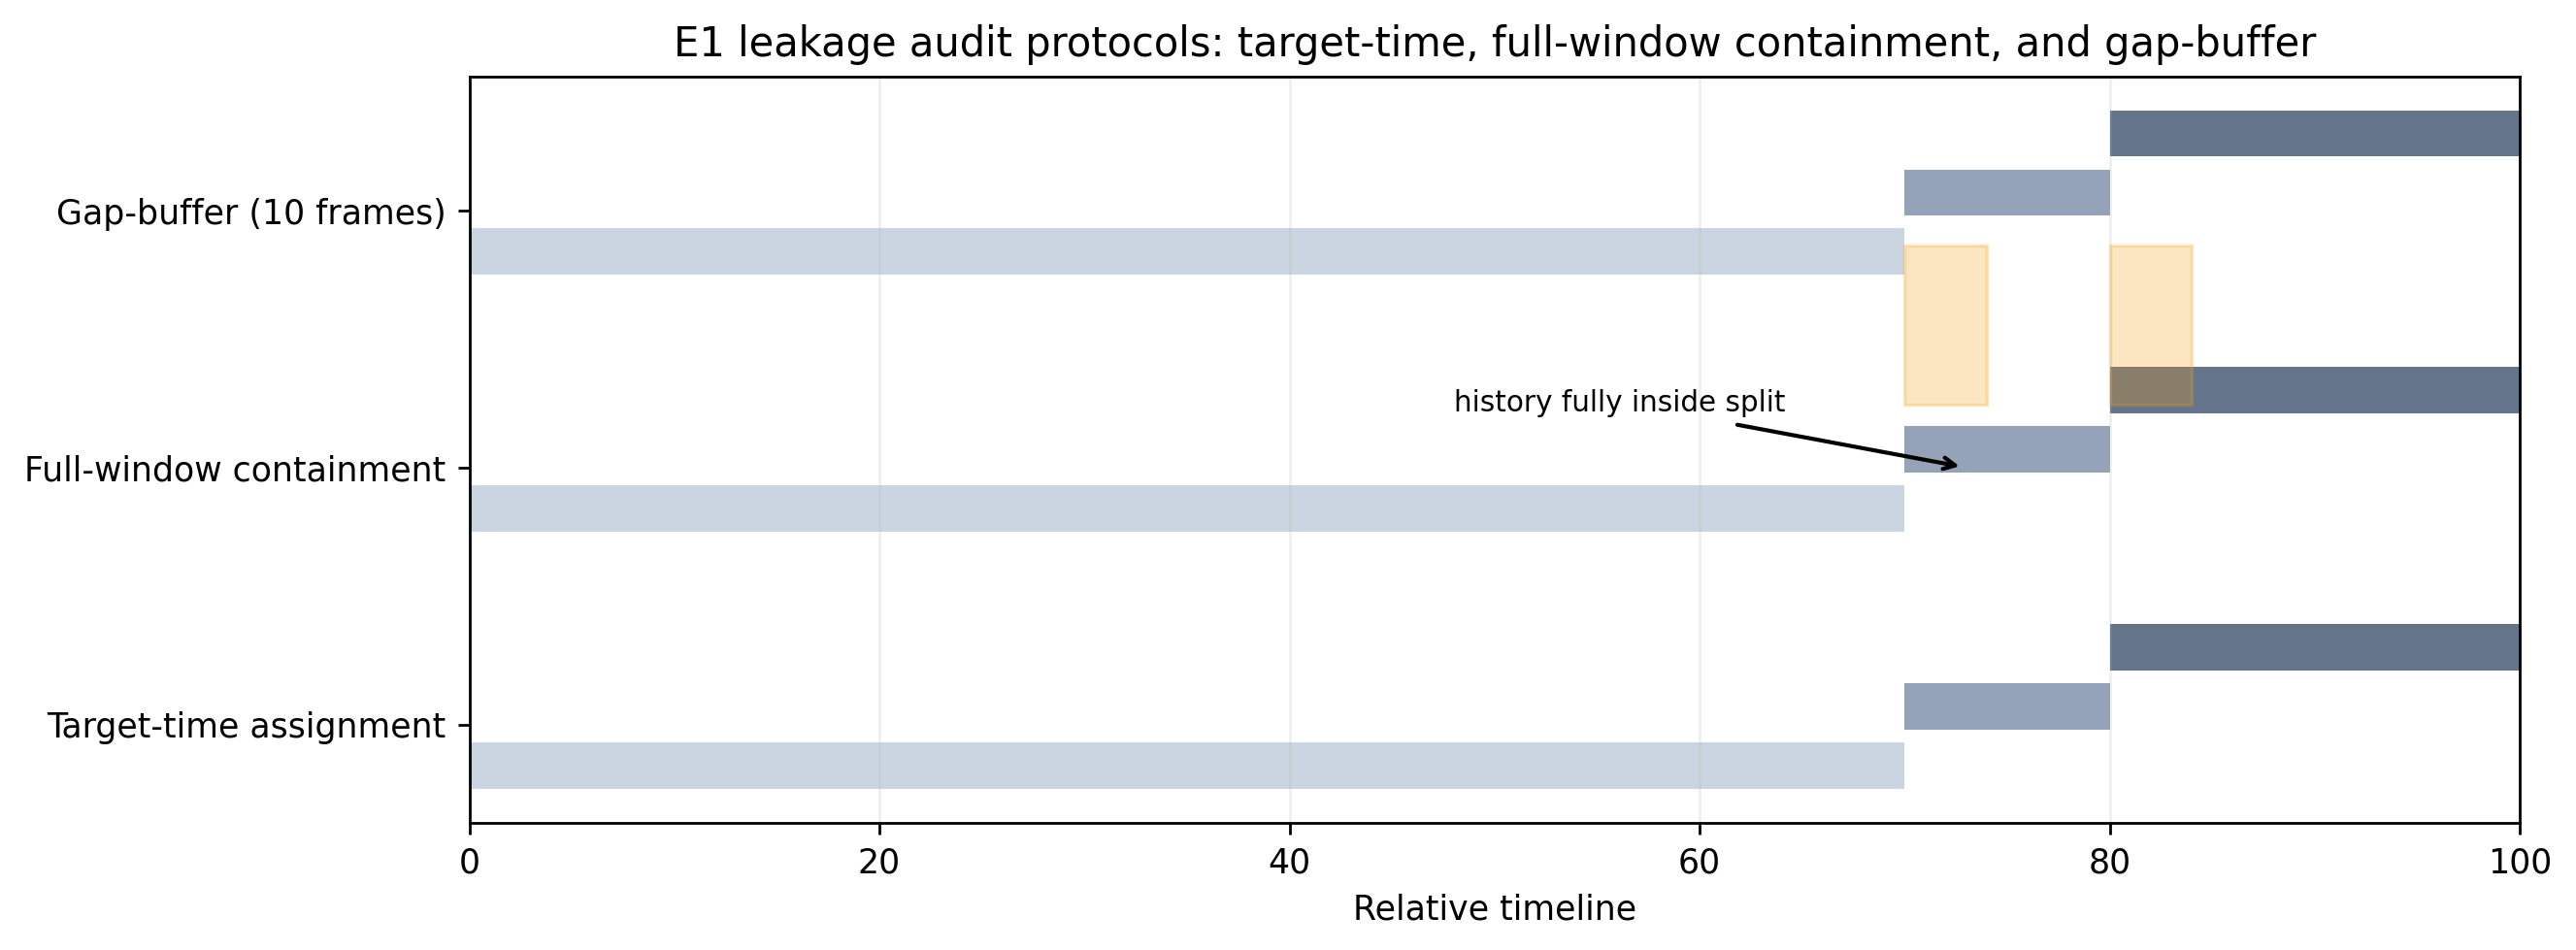
\includegraphics[width=0.95\textwidth]{paper_assets_vcea_extras/figures/E1/fig_E1_protocol_timeline.png}
\caption{Timeline illustration of the three split-protocol audit settings: target-time assignment, full-window containment, and the 10-frame gap-buffer protocol.}
\label{fig:e1_protocol_timeline}
\end{figure}

\begin{figure}[!t]
\centering
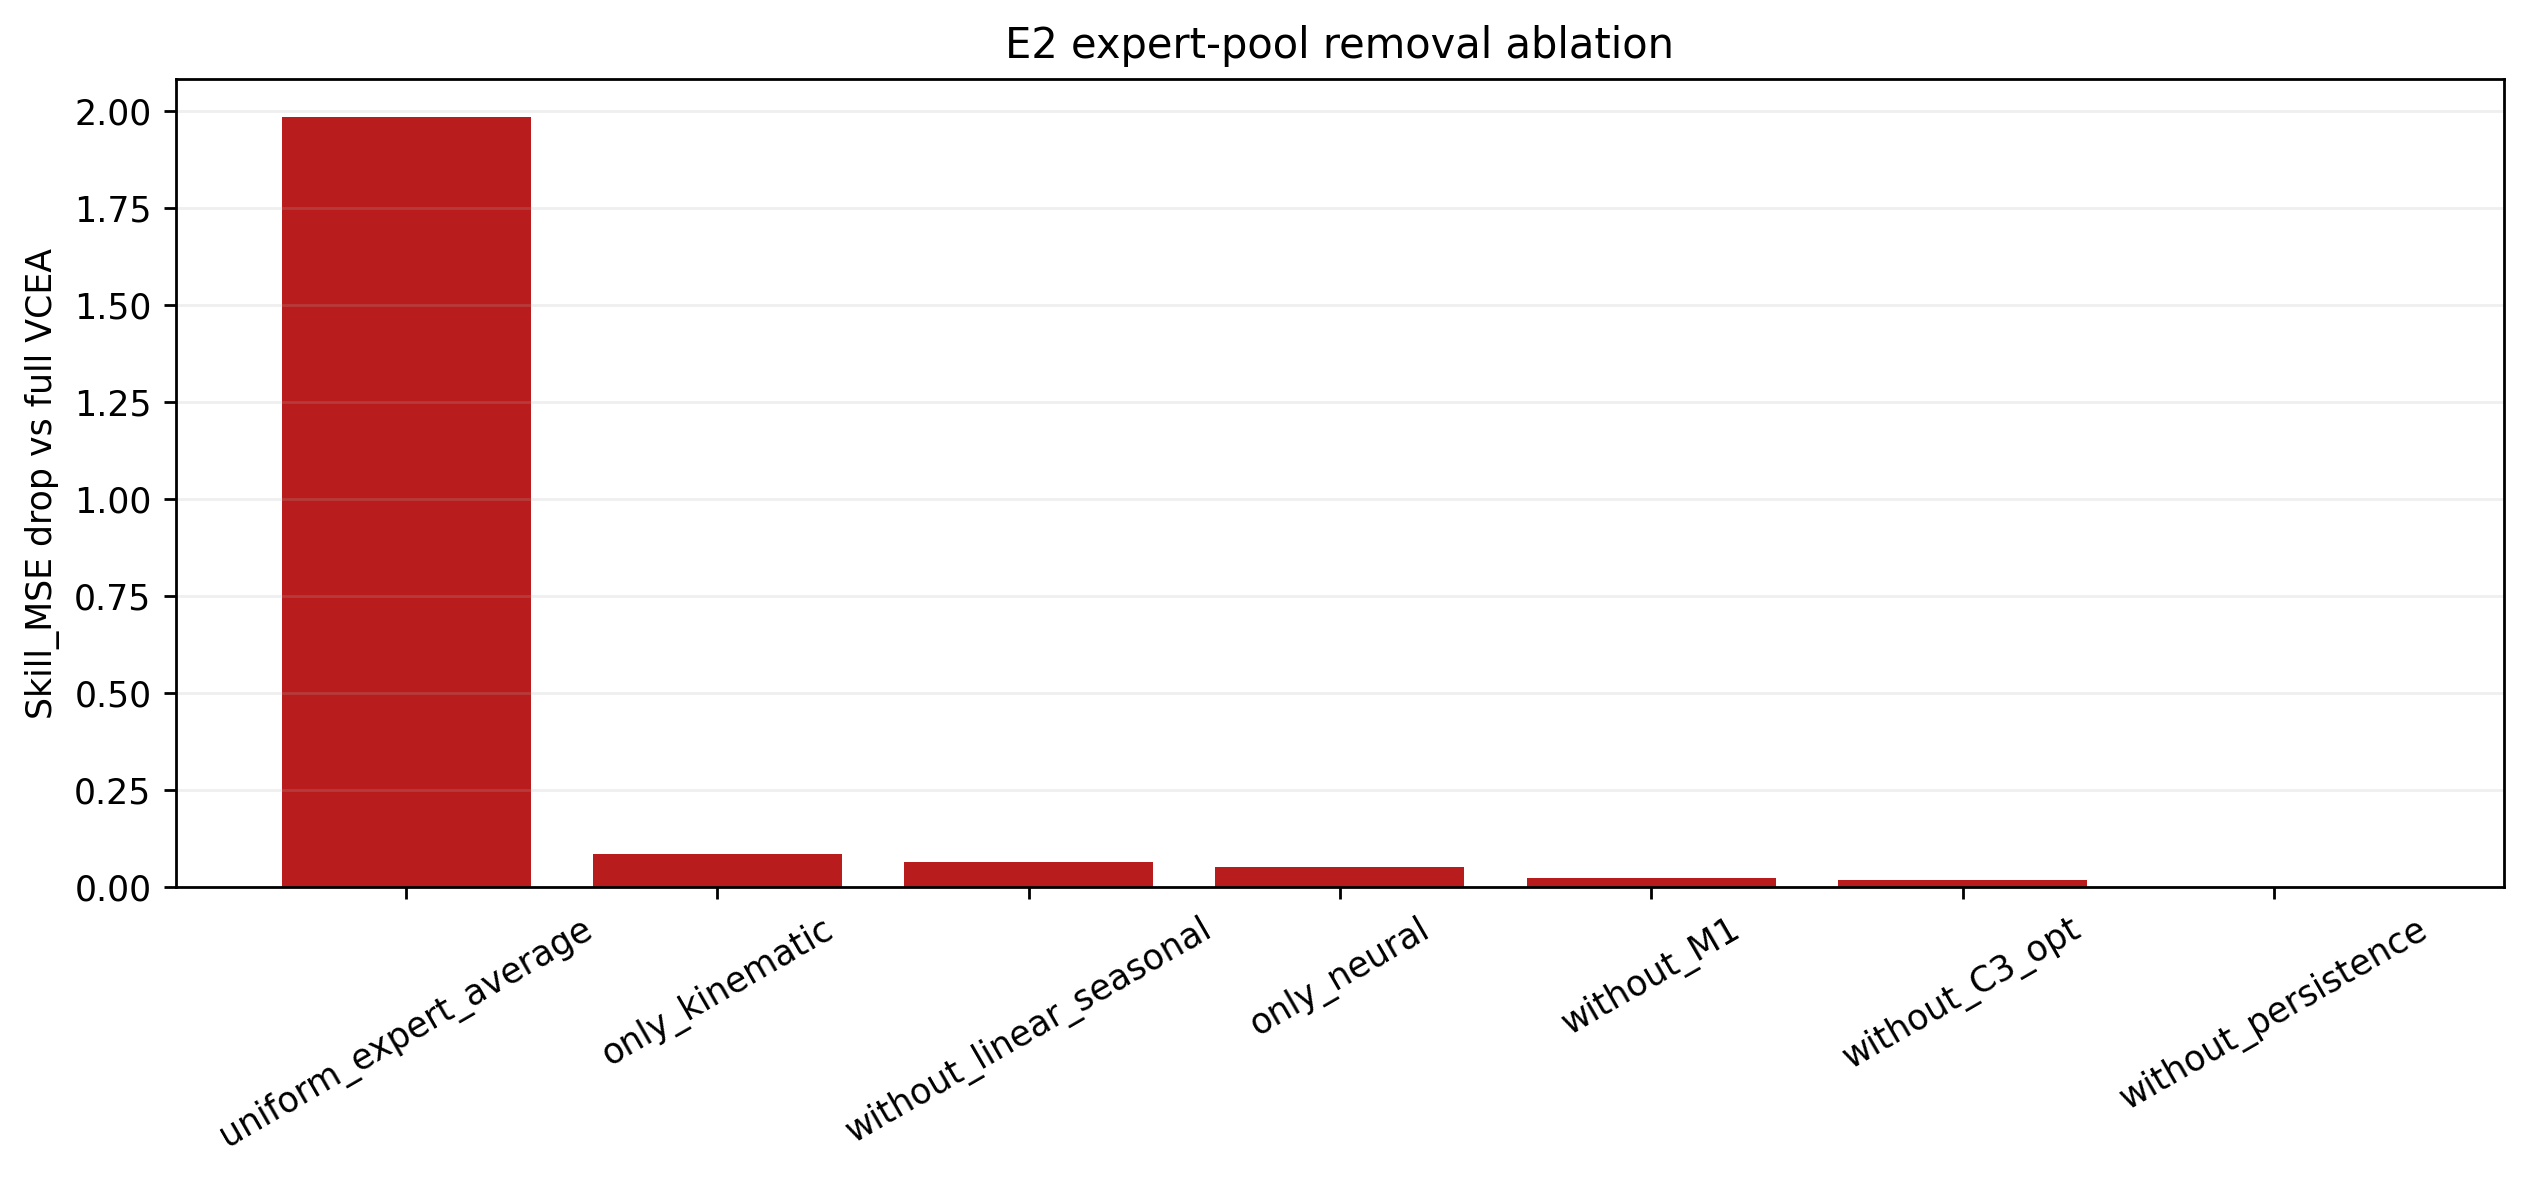
\includegraphics[width=0.95\textwidth]{paper_assets_vcea_extras/figures/E2/fig_E2_remove_expert_delta.png}
\caption{Performance change after removing individual experts from the VCEA pool.}
\label{fig:e2_remove_expert_delta}
\end{figure}

\begin{figure}[!t]
\centering
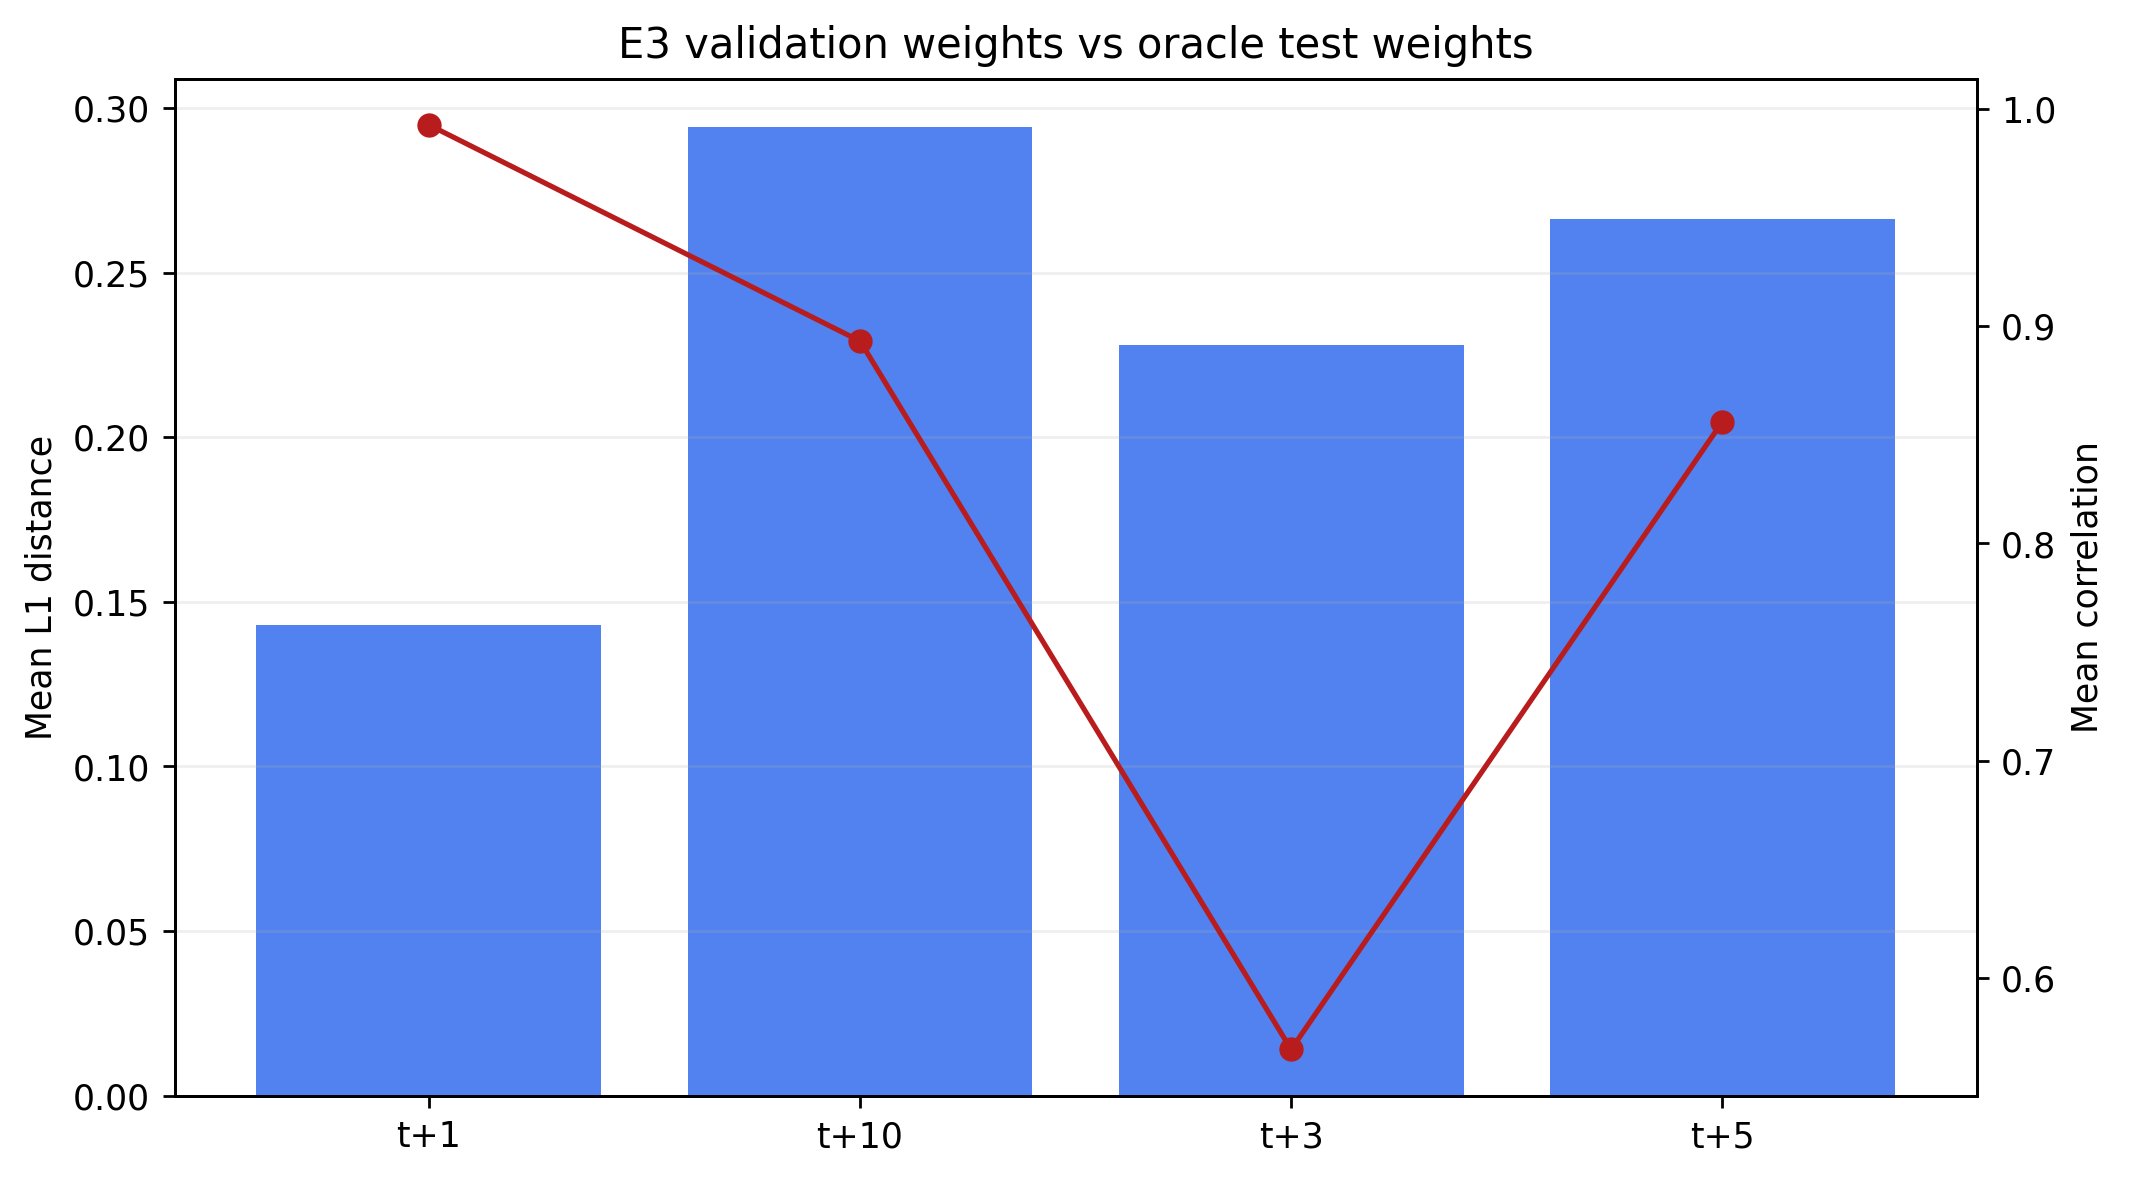
\includegraphics[width=0.95\textwidth]{paper_assets_vcea_extras/figures/E3/fig_E3_val_vs_test_weights.png}
\caption{Comparison between validation-derived weights and oracle test weights.}
\label{fig:e3_val_vs_test_weights}
\end{figure}

\begin{figure}[!t]
\centering
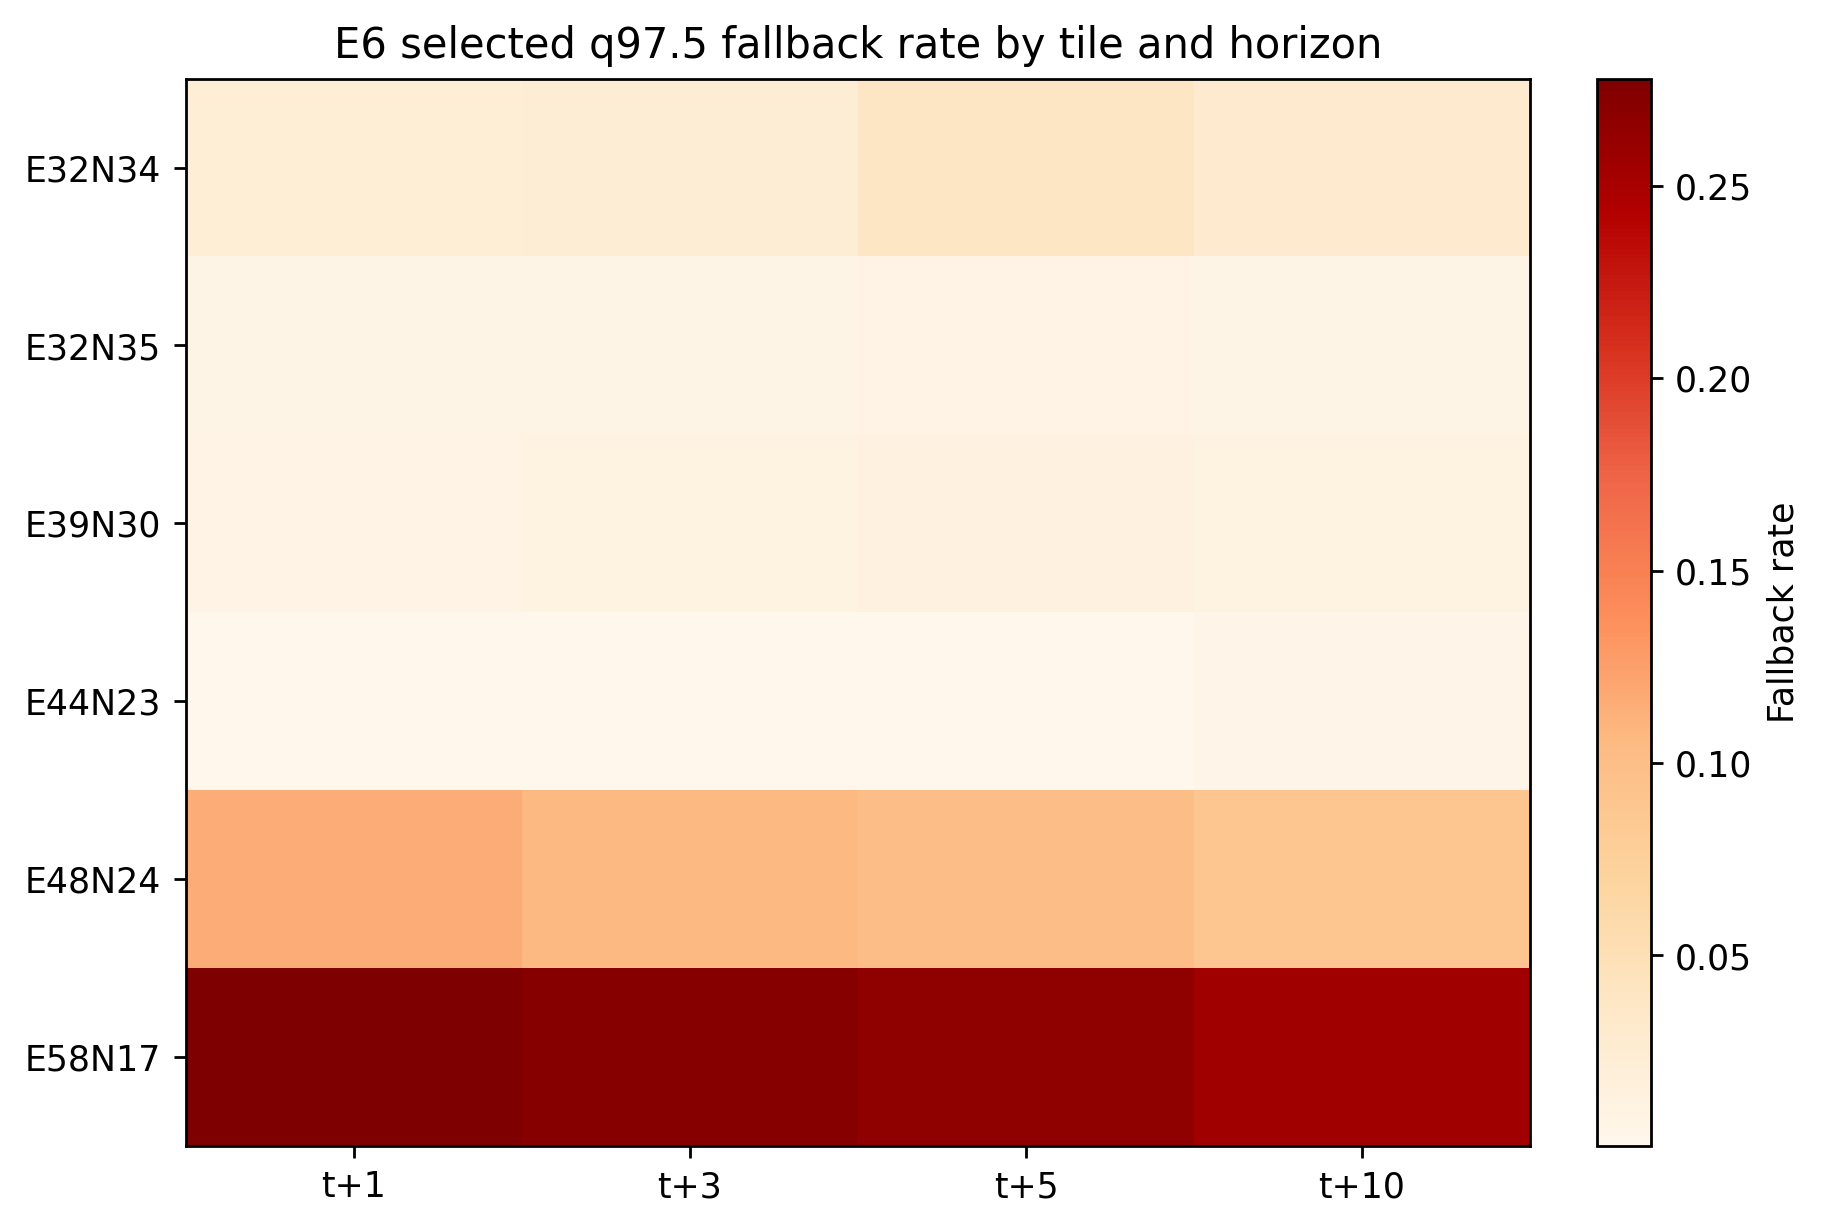
\includegraphics[width=0.95\textwidth]{paper_assets_vcea_extras/figures/E6/fig_E6_fallback_rate_by_tile.png}
\caption{Fallback rate by tile under the SS-VCEA threshold sweep.}
\label{fig:e6_fallback_rate_by_tile}
\end{figure}

\begin{figure}[!t]
\centering
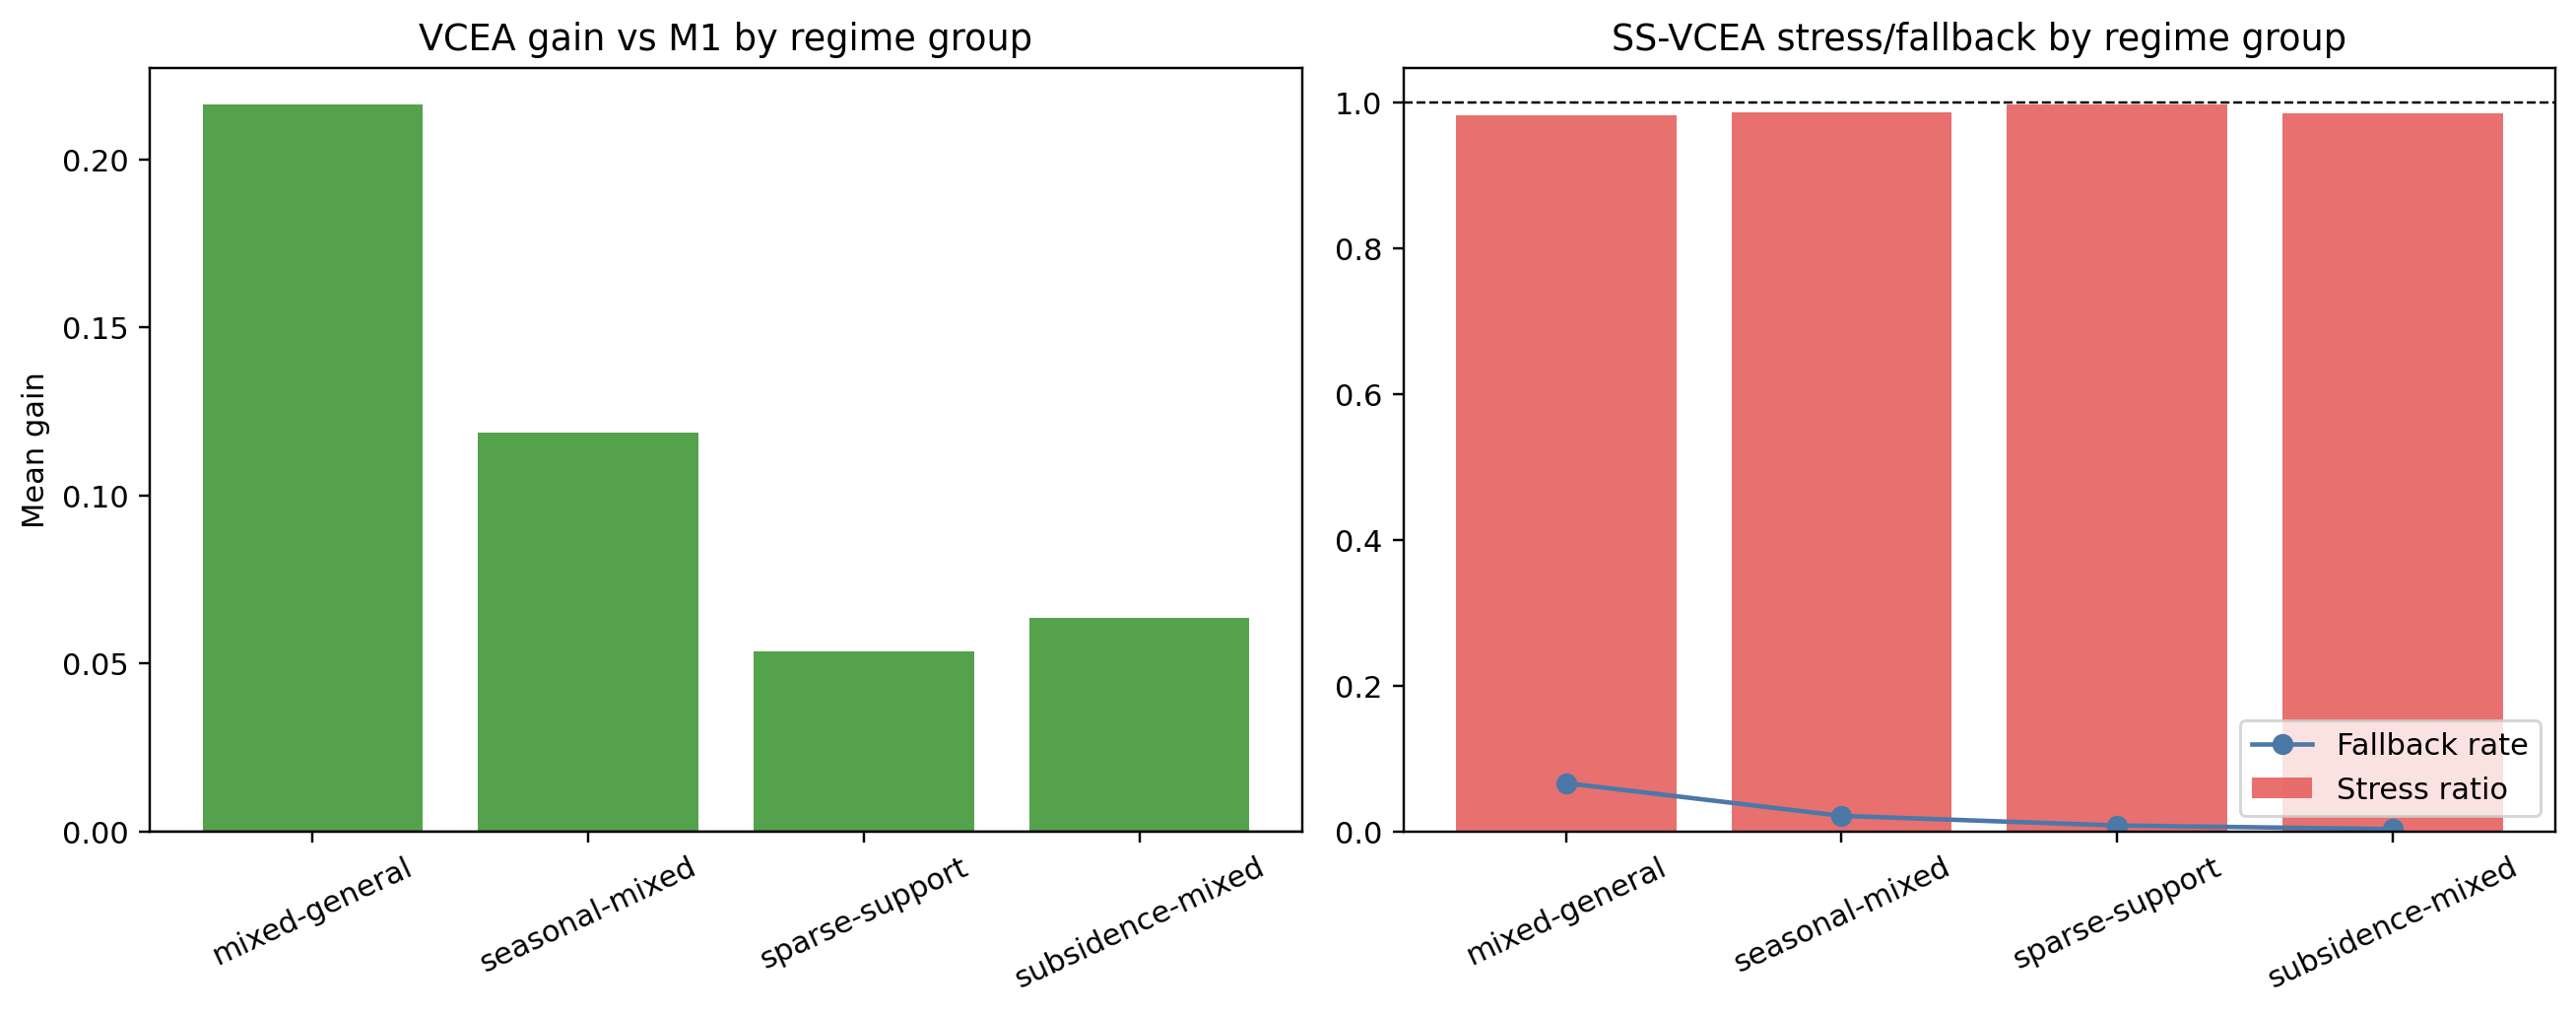
\includegraphics[width=0.95\textwidth]{paper_assets_vcea_extras/figures/E7_strong/fig_E7_skill_by_regime.png}
\caption{Performance in the 14-tile European frozen audit grouped by the four audit-regime groups.}
\label{fig:e7_skill_by_regime}
\end{figure}

\begin{figure}[!t]
\centering
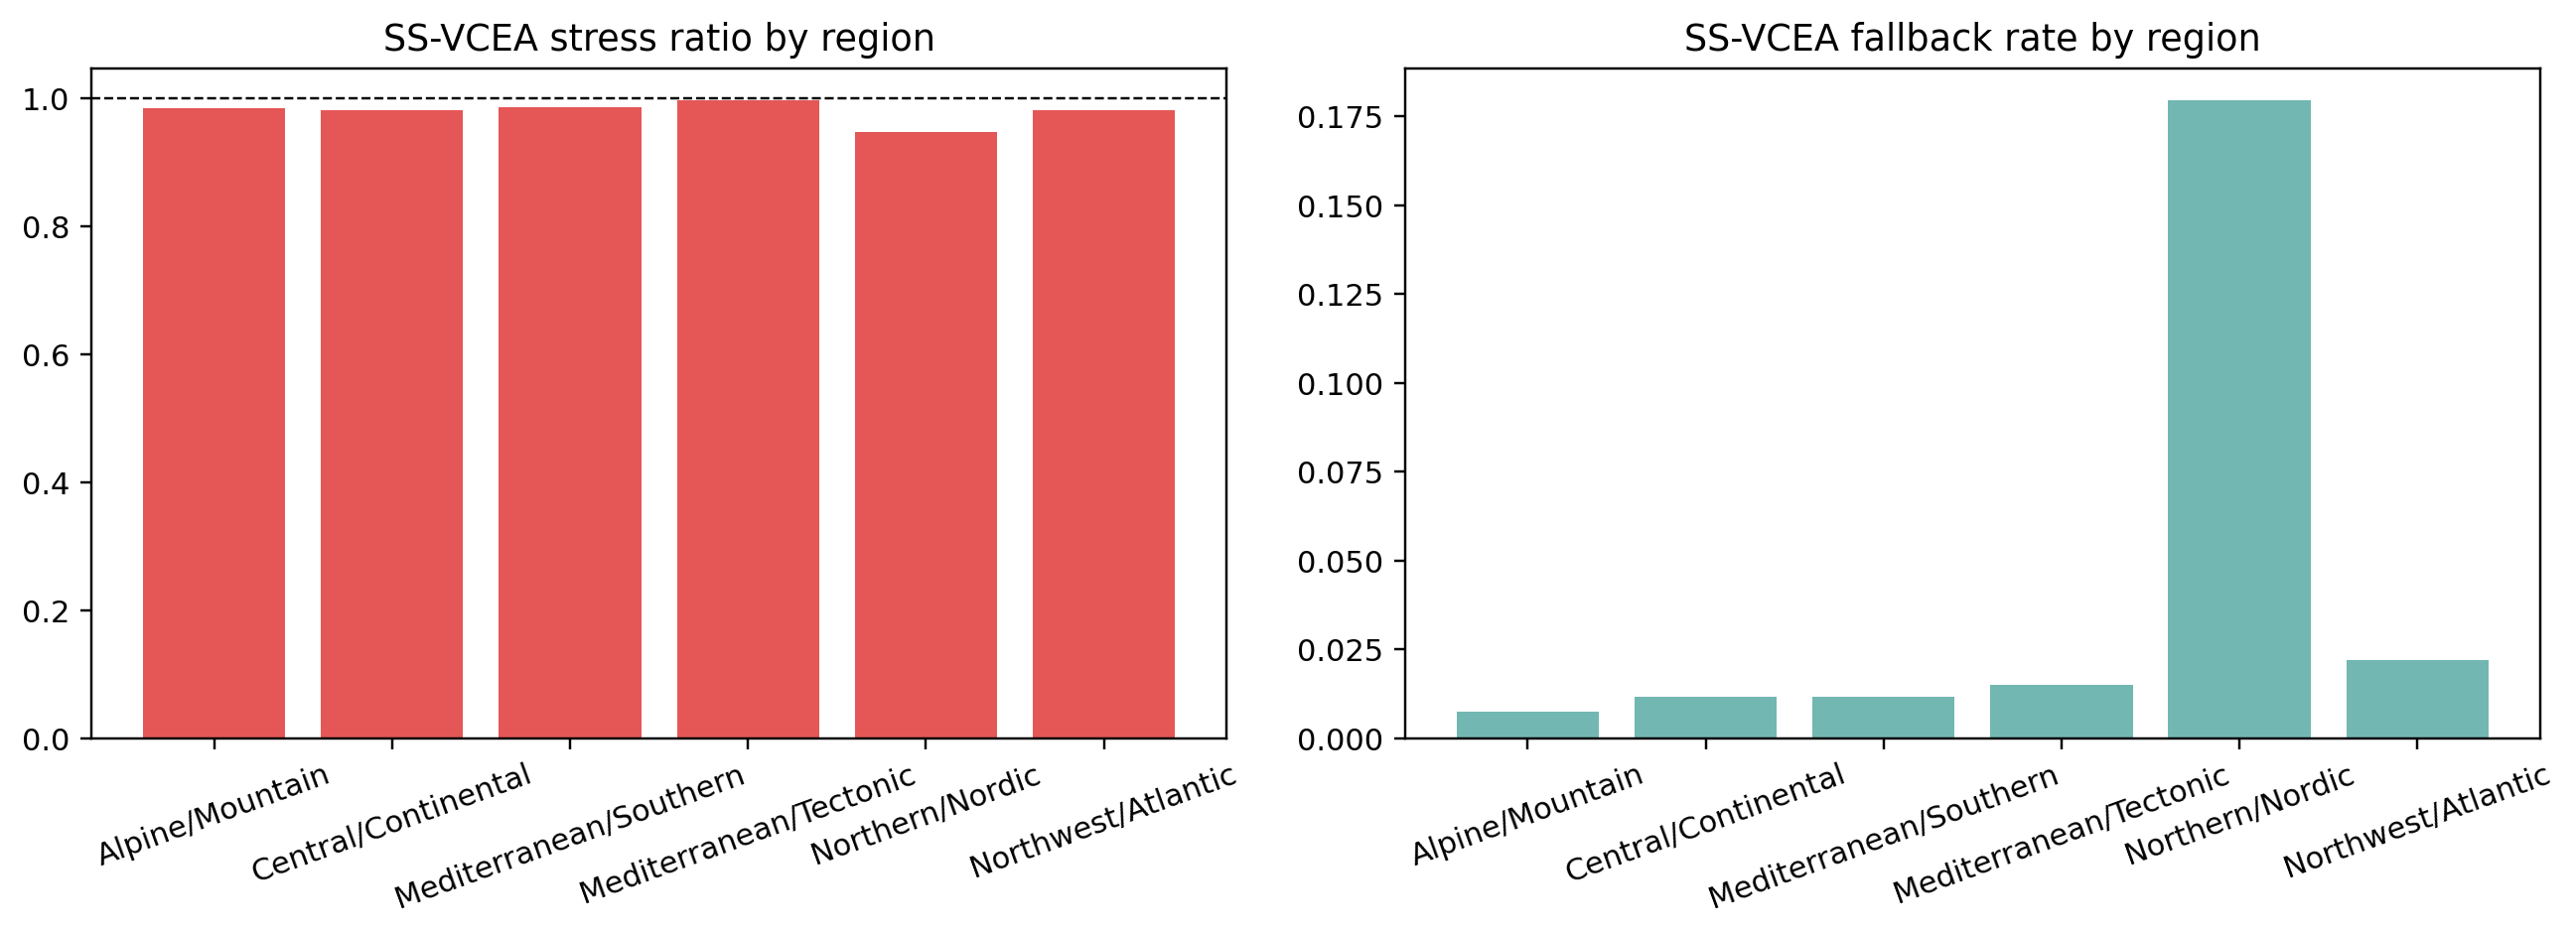
\includegraphics[width=0.95\textwidth]{paper_assets_vcea_extras/figures/E7_strong/fig_E7_stress_by_region.png}
\caption{Stress ratio and fallback rate by broad-region stratum for SS-VCEA q97.5 in the 14-tile European frozen audit.}
\label{fig:e7_stress_by_region}
\end{figure}

\begin{figure}[!t]
\centering
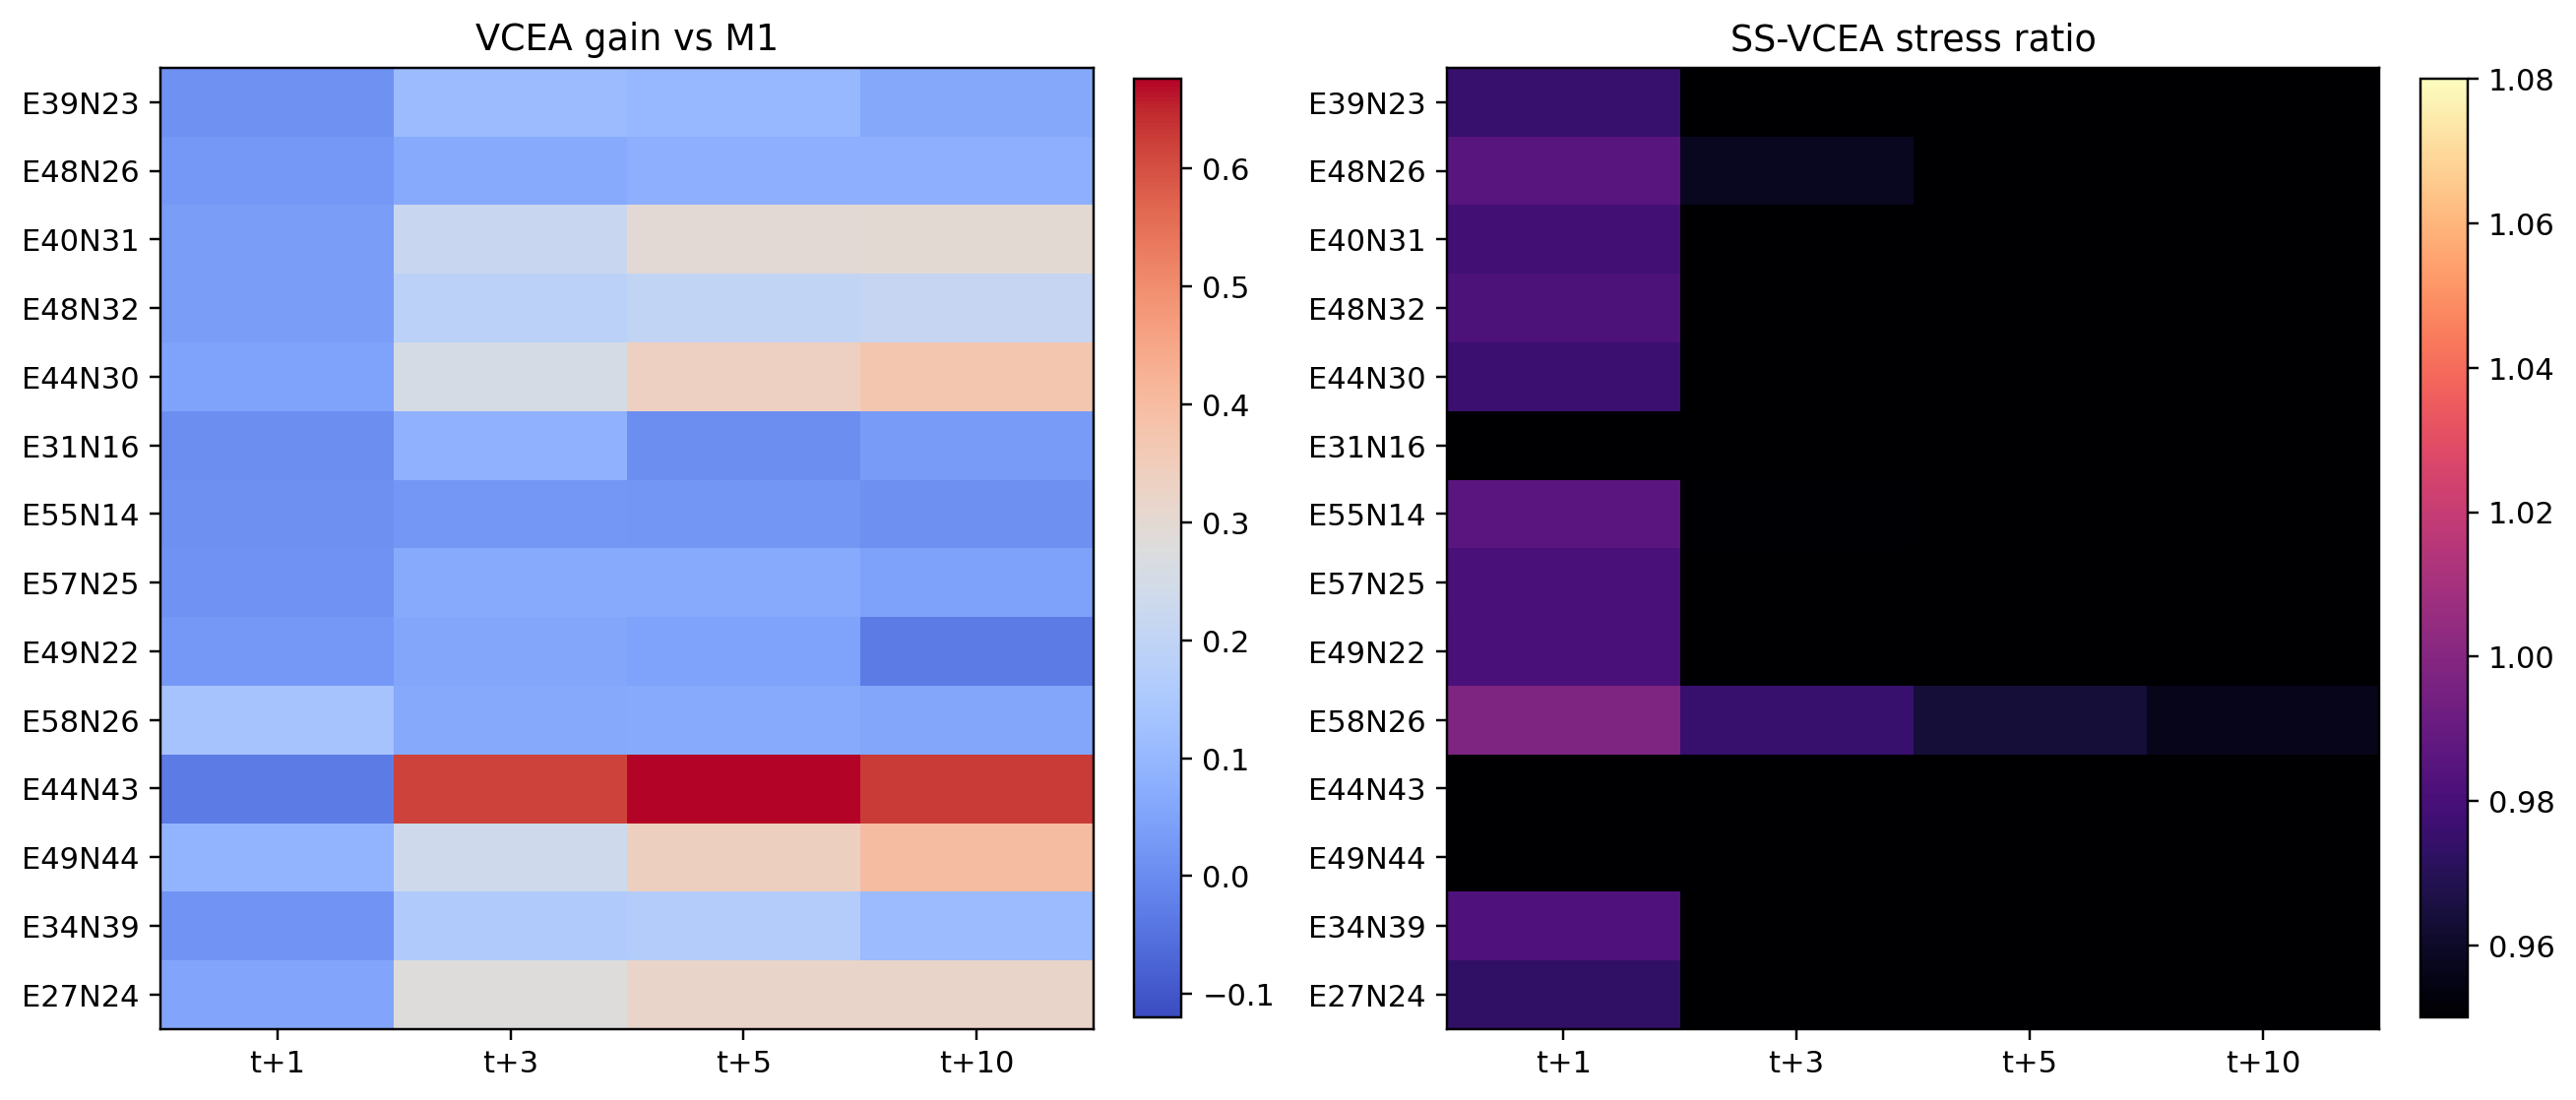
\includegraphics[width=0.95\textwidth]{paper_assets_vcea_extras/figures/E7_strong/fig_E7_failure_case_overview.png}
\caption{Overview of gains and stress across the 14 held-out EGMS 2019--2023 tiles and 56 tile-horizon evaluations in the 14-tile European frozen audit.}
\label{fig:e7_failure_case_overview}
\end{figure}



\end{document}
